\documentclass[a4paper, fleqn]{extarticle}
\usepackage{geometry}
\usepackage{Alegreya, euler}
\usepackage{microtype}
\usepackage{graphicx}
\usepackage{epstopdf}
%\usepackage{parskip}
\usepackage{amsmath}
\usepackage{amsthm}
\interdisplaylinepenalty=2500
\usepackage{amssymb}
\usepackage{hyperref}
\usepackage{comment}

\newcommand{\C}{\mathbb C}
\newcommand{\R}{\mathbb R}
\newcommand{\Q}{\mathbb Q}
\newcommand{\Z}{\mathbb Z}
\newcommand{\N}{\mathbb N}
\newcommand{\pies}{\mathcal{P}}

\input{main_tikz}

\newcounter{dummy}
\numberwithin{dummy}{section}
\newtheorem{definicja}[dummy]{Definicja}
\newtheorem{twierdzenie}[dummy]{Twierdzenie}
\newtheorem{lemat}[dummy]{Lemat}
\newtheorem{wniosek}[dummy]{Wniosek}
\newtheorem{przyklad}[dummy]{Przyklad}
\newtheorem{hipoteza}[dummy]{Hipoteza}

\usepackage[polish]{babel}
\usepackage[utf8]{inputenc}
\usepackage[T1]{fontenc}
\selectlanguage{polish}

\title{Teoria węzłów}
\author{nasze nazwiska}

\begin{document}
\maketitle
\tableofcontents

% Maciek

\newpage

\section{Rozdział Pierwszy}

Jest dość dużo (więcej niż trzy) definicji węzła. Każda z nich w pewnym sensie oddaję intuicję, która kryje się za potocznym rozumieniem nazwy tego pojęcia. W tym rozdziale podamy 
jedną z nich. 
Powiemy też, co to znaczy, że dwa węzły są równoważne, tj. zastanowimy się, kiedy mając dane dwa węzły jesteśmy wstanie równoważnie (nie zmieniając ''ciągłej struktury'') 
zdeformować jeden z nich, aby otrzymać drugi. Zastanowimy się nad tym, jakie przekształcenia możemy uważać za takie deformacje. Na koniec sformułujemy i udowodnimy 
twierdzenie Reidemeistera.

\subsection{Definicja}

Zaczniemy ten rozdział do sformuowania definicji węzła. Kiedy definiuje się matemayczne pojęcie ważne jest (przynajmniej takie wrażenie ma autor tej części pracy), 
żeby definicja odpowiadała naszym oczekiwaniom, tj. żeby gwarantowała oczekiwane własności, a jednocześnie zachowywała możliwie jak największy 
stopień ogólności. 

Na pierwszy rzut oka następujące podejście wygląda dość rozsądnie.


\begin{definicja}
\label{zla_definicja}
 Węzłem nazywamy ciągłą funkcję $f\colon[0,1]\to\mathbb{R}^3$, która spełnia następujące własności:
 \begin{enumerate}
  \item $f(0) = f(1)$,
  \item $\forall x,y\in[0,1) \ \ \ f(x) = f(y)\Rightarrow x = y$.
 \end{enumerate}
\end{definicja}

W rzeczywistości ma ono dość poważne wady.
Po pierwsze, powyższa definicja dopuszcza tak zwane dzikie węzły (rysunek poniżej), co jest sprzeczne z intuicyjnym pojmowaniem węzła, który może mieć 
jedynie skończenie wiele pętli. 


	\begin{center}

	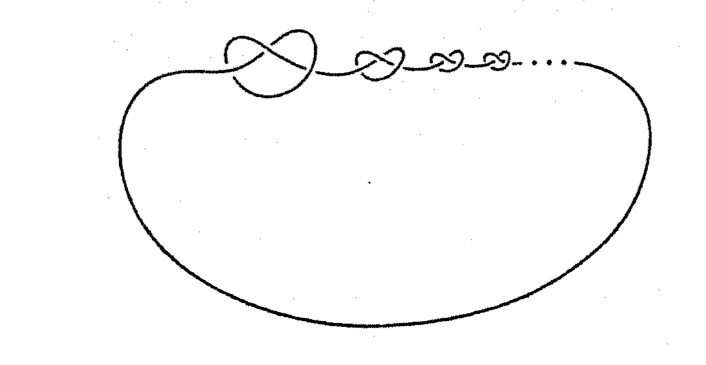
\includegraphics[scale=0.3]{1/pictures/wild.png}
	\end{center}


Po drugie wychodząc od definicji \ref{zla_definicja} mielibyśmy kłopot z określeniem tego, kiedy dane dwa węzły są równoważne. Naturalną definicją wydaje się
następująca: węzły $K$ i $J$ uważamy za równoważne, gdy istnieje rodzina węzłów $\lbrace K_t\rbrace_{t\in[0,1]}$, taka że $K_0 = K$, oraz $K_1 = J$. Oprócz tego 
węzły $K_t$ i $K_s$ powinny leżeć dowolnie ''blisko'' dla $t$ dostatecznie bliskich $s$. W sensie tej definicji (nie wnikając w to, co oznacza,
że dwa węzły leżą ''blisko''), moglibyśmy sciągnąć pojedynczą pętlę do okręgu (patrz rysunek poniżej). 


	\begin{center}
	
	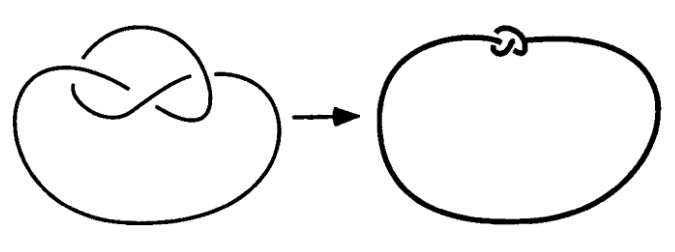
\includegraphics[scale=0.6]{1/pictures/loop.png} 
	\end{center}


Rozwiązanie naszych problemów okazuje się zaskakująco proste. Zamiast definiować węzeł za pomocą ciągłej krzywej, moża posłużyć się łamaną. Skąd tem pomysł? Łamana ma skończenie wiele
wierzchołków, zatem powinniśmy bez specjalnych problemów wykluczyć z naszych rozważań tak zwane dzikie węzły. Takie dyskretne podejście pozwoli nam też stosunkowo w prosty sposób zdefiniować
pojęcie elementarnej deformacji.



\begin{definicja}
 Odcinkiem domkniętym łączącym parę różnych punktów $p,q\in\mathbb{R}^3$ nazwiemy zbiór 
 \begin{displaymath}
  [p,q] := \lbrace \lambda p + (1-\lambda)(q-p): \lambda\in[0,1]\rbrace.
 \end{displaymath}
\end{definicja}

\begin{definicja}
 Niech $p_1, p_2, \ldots, p_n\in\mathbb{R}^3$ będą parami różne. Łamaną o wierzchołkach $p_i$ nazwiemy zbiór 
 \begin{displaymath}
  \bigcup_{i=1}^n [p_i, p_{i+1}].
 \end{displaymath}
 Łamaną tej postaci będziemy oznaczać przez $(p_1, p_2, \ldots, p_n)$. Gdy $p_1 = p_n$ mówimy o łamanej zamkniętej.
 Jeśli dodatkowo każdy punkt łamanej należy do dokładnie jednego odcinka, mówimy wtedy o łamanej bez samoprzecięć. Jeśli dodatkowo $p_1 = p_n$, wówczas mówimy o łamanej
 zamkniętej bez samoprzecięć. Odcinek $[p_i, p_{i+1}]$ będziemy dalej krótko oznaczać przez $I_i$.
\end{definicja}

\begin{definicja}
 Węzeł to łamana zamknięta w $\mathbb{R}^3$ bez samoprzecięć.
\end{definicja}

\textbf{Uwaga} Jeśli węzeł $K$ to łamana $(p_1, p_2, \ldots, p_n)$, wówczas zbiór $(p_{\sigma(1)}, p_{\sigma(2)},\ldots, p_{\sigma(n)})$, gdzie $\sigma$ to cykl długości $n$
definiuje ten sam węzeł $K$.
Co więcej, jeśli dla pewnego $i$ punkty $p_{i-1}, p_i, p_{i+1}$ są współliniowe, to oczywiście $K = (p_1, p_2, \ldots, p_{i-1}, p_{i+1}, \ldots, p_n)$. Z ostatniego spostrzeżenia łatwo
można wywnioskować, że węzeł jest jednoznacznie wyznaczony przez minimalny (w sensie inkluzji) zbiór wierzchołków łamanej, która ten węzeł definiuje. 

\begin{definicja}
 Niech uporządkowany zbiór $(p_1, p_2,\ldots, p_n)$ definiuje węzeł $K$. Jeśli żaden jego właściwy podzbiór nie definiuje tego samego węzła $K$, wówczas elementy zbioru $\lbrace p_1, p_2, \ldots, p_n\rbrace$
 nazwiemy wierzchołkami węzła $K$.
\end{definicja}

Od tego momentu będziemy definiować węzeł poprzez łamane o minimalnej liczbie wierzchołków, chyba, że zostanie powiedziane inaczej. Na koniec tego podrozdziału podamy definicję splotu.

\begin{definicja}
 Splotem nazywamy sumę (mnogościową) skończenie wielu parami rozłącznych węzłów. Każdy taki węzeł nazywamy składową splotu. W szczególności węzeł jest splotem o jednej skłądowej. 
\end{definicja}

\subsection{Równoważność węzłów}
W tym podrozdziale zastanowimy się nad tym, kiedy dwa, pozornie różne węzły, w istocie możemy uważać za takie same (mimo iż explicite nie są tym samym węzłem). 
Zaczniemy od zdefiniowania kilku pojęć.

\begin{definicja}
\label{elementarne_p}
 Niech dane będą węzły $J = (p_0, p_1, p_2, \ldots, p_n)$ oraz $K = (p_1, p_2, \ldots, p_n)$. 
 Powiemy, że $J$ powstaje przez elementarną deformację węzła $K$ gdy: 
 \begin{enumerate}
  \item punkt $p_0$ nie jest współliniowy z $p_{1}$ oraz z $p_{n}$,
  \item część wspólna trójkąta (trójkąt rozumiemy jako trójkąt z wnętrzem) o wierzchołkach w punktach $p_0, p_1, p_n$ z węzłem $K$ zawiera się w odcinku $[p_1, p_n]$.
 \end{enumerate}
 Przekształcenie odwrotne do elementarnej deformacji również jest elementarną deformacją.
\end{definicja}
\textbf{Uwaga} Powyższą definicję można uogólnić zastępując węzeł $K$ węzłem $(p_1,\ldots, p_{i-1},p_{i+1}, \ldots, p_n)$ dla $i = 1,2,\ldots n-1$, oraz zastępując wierzchołki
$p_0, p_1, p_n$ wierzchołkami $p_i, p_{i+1}, p_{i-1}$ odpowiednio.

\begin{definicja}
 Mówimy, że węzły $J$ i $K$ są równoważne, gdy istnieje skończony ciąg węzłów $K_0, K_1, \ldots, K_n$, gdzie $K_0$ = $K$, $K_n = J$, oraz $K_{i+1}$ jest elementarną
 deformacją węzła $K_i$. 
\end{definicja}

Sprawdzenie, że podana relacja jest w istocie relacją równoważności pozostawiamy czytelnikowi jako proste ćwiczenie.

Dla przykładu rozważmy dowolny $n$-kąt wypukły na płaszczyźnie. Można łatwo pokazać przez indukcję (po liczbie wierzchołków), że każdy taki wielokąt jest równoważny trójkątowi. 
Istotnie, dla trójkąta
teza jest oczywista. Załóżmy jej prawdziwość dla wszystkich liczb naturalnych nie większych, niż $n$. Mając dowolny $n+1$-kąt wypukły $J = (k_0, k_1, k_2, \ldots, k_n)$ łatwo się przekonać,
że jest on elementarnym przekształceniem $n$-kąta $ K = (k_1, k_2, \ldots, k_n)$. To, że $K$ jest wielokątem wypukłym, podobnie jak to, że pierwszy warunek z definicji \ref{elementarne_p} jest spełniony, jest oczywiste.
Drugi warunek jest spełniony, ponieważ z wypukłości $K$ zachodzi $\left([p_0,p_1]\cup [p_0, p_n]\right) \cap K = \lbrace p_1, p_n\rbrace$.

\begin{definicja}
 Każdy węzeł, który jest elementem klasy abstrakcji opisanej w przykładzie nazywamy niewęzłem.
\end{definicja}
\begin{definicja}
 Sploten trywialnym nazywamy sumę mnogościową skończenie wielu rozłącznych niewęzłów leżących w jednej płaszczyźnie.
\end{definicja}

\textbf{Uwaga} W przypadku nie-splotu warunek leżenia w jednej płaszczyźnie jest istotny. Aby się o tym przekonać czytelnik może zechcieć odpowiedzieć na pytanie, 
jak mogą leżeć względem siebie rozłączne okręgi w $\mathbb{R}^3$, a jak muszą w $\mathbb{R}^2$.

Od tej chwili węzły równoważne będziemy uważać za tożsame, to znaczy zamiast pisać, że węzeł $J$ jest równoważny węzłowi $K$, będziemy pisać krótko $J=K$ (właśnie w taki sposób
został powyżej zdefiniowany niewęzeł).
Odróżniać będziemy tylko te węzły, które nie są równoważne. 

\subsection{Diagram}
Od początku tej pracy, z konieczności rysowaliśmy węzły (obiekty żyjące w przestrzeni trójwymiarowej) na płaszczyźnie. 
W tym podrozdziale podamy ścisłą definicję tych dwuwymiarowych rysunków (diagramów) i pokażemy, że jeśli dwa węzły mają przedstawienie w postaci tego samego diagramu, 
to są w istocie równoważne.

\begin{definicja}
 Rzutem zbioru $A\subseteq\mathbb{R}^3$ na płaszczyznę nazwiemy funkcję $p\colon A\to\mathbb{R}^2$ określoną wzorem $p(x,y,z) = (x,y)$. Kiedy $A$ jest węzłem, $p[A]$ nazywamy 
 rzutem węzła $A$ na płaszczyznę.
\end{definicja}


\begin{definicja}
\label{rzut_reg}
 Rzutem regularnym węzła $K$ nazywamy takie rzutowanie $p$ węzła $K$ na płaszczyznę, że
 \begin{enumerate}
  \item dla każdego wierzchołka $v$, dla każdego $a\in K$ jeśli $p(v) = p(a)$, to $p=a$,
  \item dla każdych $a_1, a_2, a_3$ jeśli $p(a_1)=p(a_2)=p(a_3)$, to $a_1=a_2$ lub $a_1=a_3$ lub $a_2=a_3$.
 \end{enumerate}
\end{definicja}

Zakładająć, że węzeł ma regularny rzut na płaszczyznę, możemy w ścisły sposób zdefiniować pojęcie diagramu.
Diagramem węzła $K$ nazywamy następującą modyfikację regularnego rzutu $K$ na płaszczyznę. Jeśli przeciwobrazem punktu $(x_0, y_0)$ jest zbiór dwuelementowy 
$\lbrace a,b\rbrace$, wówczas w tym punkcie przecinają się dwa różne odcinki, które są rzutami dwóch różnych odcinków węzła $K$, powiedzmy $I_a, I_b$. 
Ponieważ rzut $K$ jest rzutem regularnym, więc jeden z tych odcinków leży pod drugim, co oznaczamy, jak na poniższym rysunku. \\


	\begin{center}

	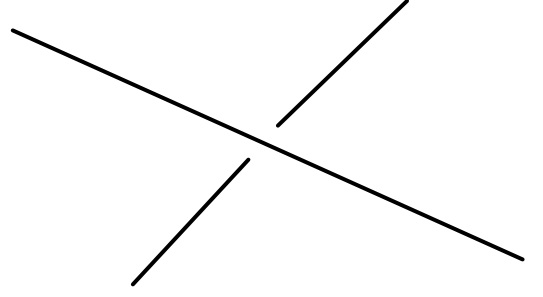
\includegraphics[scale=0.4]{1/pictures/skrz.jpg}
	\end{center}


\begin{definicja}
 Mówimy, że dwa węzły $(p_i)$, $(q_j)$ są od siebie odległe o mniej, niż $t$, gdy mają tyle samo wierzchołków i gdy dla każdej pary wierzchołków zachodzi $d(p_k,q_k) < t$.
\end{definicja}

Udowodnimy teraz twierdzenie, które zagwarantuje nam, że dla każdego węzła można znaleźć węzeł dowolnie mu bliski, który jest równoważny z wyjściowym, i którego rzut na płaszczyznę jest regularny. 
Będziemy do tego potrzebować następujących lematów.

\begin{lemat}
\label{LEM1}
 Dla dowolnego węzła $K = (v_0, \ldots, v_i, \ldots, v_n)$ i dowolnego $i\in\lbrace 1,2,\ldots n\rbrace$ istnieje taki $\epsilon > 0$, że dla każdego $v'\in B(v_i, \epsilon)$ 
 węzły $K$ oraz $(v_0, \ldots,v_{i-1}, v', v_{i+1}, \ldots, v_n)$ są równoważne.
\end{lemat}
\begin{proof}

Ustalmy dowolne $i$. Dodawanie i odejmowanie indeksów w dalszej części dowodu należy rozumieć jak działanie modulo $n+1$. Możemy założyć, że punkty $v_{i-1}, v_i, v_{i+1}$ nie są
współliniowe. Zaczniemy dowód od skonstruowania dwóch stożków.
Stożek o wierzchołku $w$, środku podstawy $s$ i promieniu podstawy $r$ będę oznaczał $S(s,r,w)$. 

Niech $p\in\mathbb{R}^3$ będzie wektorem długości jeden prostopadłym do odcinków $I_{i-1}$ oraz $I_i$. Oznaczmy przez $\alpha$ kąt pomiędzy odcinkami 
$I_{i-2}$ i $I_{i-1}$. 
Dobierzmy tak małą $\mu\in\mathbb{R}^3$, żeby kąt pomiędzy $I_{i-1}$ oraz $[v_{i-1}, v_i + \mu p]$ był mniejszy od $\alpha$. Możemy $\mu$ wyliczyć np. używając trygonometrii 
w trójkącie prostokątnym o wierzchołkach $v_{i-1}, v_i, v_i + r\cdot p$, gdzie $r\in\mathbb{R}_+$. Połóżmy
\begin{displaymath}
 \epsilon = \frac{1}{2}\min\lbrace d(I_{i-1}, K\setminus(I_{i-2}\cup I_i)), \mu\rbrace, \hbox{ oczywiście }\epsilon>0.
\end{displaymath}
Wtedy
\begin{enumerate}
 \item $S(v_i, \epsilon, v_{i-1})\cap K \subseteq I_{i-1}\cup I_i$,
 \item dla każdej $\delta\in(0,\epsilon)$ zachodzi $[v_{i-1}, v_i+\delta p]\subseteq S(v_i, \epsilon, v_{i-1})$.
\end{enumerate}
Zauważmy, że $d(v_i, cl(K\setminus(I_{i-1}\cup I_i)) > 0$, więc (jako że $\mathbb{R}^3$ jest $T_4$) można znaleźć takie
$\gamma > 0$, że $B(v_i,\gamma)\cap cl(K\setminus(I_{i-1}\cup I_i)) = \emptyset$. Możemy wziąć takie $\gamma$, żeby $\gamma < \epsilon$.

Wtedy stożek 
$S_{i-1} = S(v_i + \gamma(v_i-v_{i-1}), \epsilon, v_{i-1})$ spełnia własność $1$ oraz własność
\begin{displaymath}
 \hbox{dla każdego }v'\in B(v_i, \gamma) \ \ [v_{i-1}, v']\subseteq S_{i-1}.
\end{displaymath}


W analogiczny sposób konstruujemy stożek $S_i = S(v_i + \gamma'(v_i - v_{i+1}), \epsilon', v_{i+1})$. Zbiory $S_{i-1}$ i $S_i$ mają niepuste wnętrza, oraz 
$v_i\in int(S_i)\cap int(S_{i+1})$. Istnieje więc taka liczba $r>0$, że $B(v_i, r)\subseteq S_i\cap S_{i+1}$.

Owe stożki pomogą nam pokazać, że dla każdego $v'\in B(v_i, r)$ węzeł $(v_1, \ldots, v', \ldots, v_n)$ jest równoważny $K$.

Ustalmy $v'\in B(v_i, r)$. Wtedy odcinki $[v_{i-1}, v'], [v',v_i], [v', v_{i+1}]$ należą do zbioru $S_i\cup S_{i-1}$, który jest rozłączny z $K\setminus(I_{i-1}\cup I_i)$. 
Rozważmy dwa przypadki. 

Jeżeli $v'\in I_i$ (gdy $v'\in I_{i-1}$, to postępujemy analogicznie), to węzeł $K$ można zdefiniować za pomocą łamanej $(v_1, \ldots, v_i, v', v_{i+1}, \ldots, v_n)$. Ponieważ
wnętrze odcinka $[v_{i-1}, v']$ jest rozłączne z $K$, więc $K$ jest równoważny węzłowi $(v_1, \ldots, v_{i-1}, v', v_{i+1}, \ldots, v_n)$.

Jeśli $v'\not\in I_i\cup I_{i-1}$, wówczas wnętrze odcinka $[v_i, v']$ jest rozłączne z $I_i\cup I_{i-1}$. Rozważmy odcinek $[v_{i-1}, v']$, jeśli przecina on odcinek $I_i$, to 
wtedy odcinek $[v', v_i]$ nie przecina odcinka $I_{i-1}$, zatem bez zmniejszenia ogólności możemy założyć, że wnętrze odcinka $[v_{i-1}, v']$ jest rozłączne z $K$. Tworzymy
następujący ciąg
\begin{displaymath}
 K_0 = K, K_1 = (v_1,\ldots, v_{i-1}, v', v_i, \ldots, v_n), K_2 = (v_1,\ldots, v_{i-1}, v', v_{i+1}, \ldots, v_n).
\end{displaymath}
Czytelnik zechce się sam przekonać, że jest to ciąg elementarnych deformacji. 
Kładziemy $K' = K_2$ i kończymy dowód.
\end{proof}
\textbf{Uwaga} Ponieważ funkcja
 $ d(x,y)\mapsto d(p(x), p(y))$ jest nierosnąca, więc przy oznaczeniach, jak w dowodzie lematu zachodzi $p(v')\in B(p(v_i),\epsilon)$.

\begin{lemat}
 \label{LEM2}
 Rozpatrzmy węzeł $K = (v_1, \ldots, v_n)$. Niech $p$ oznacza rzut na płaszczyznę. Dla każdego $i$, dla każdego $\epsilon > 0$ istnieje węzeł
 węzeł $J = (q_1, \ldots, q_i, \ldots q_n)$ równoważny węzłowi $K$ odległy od $K$ o mniej niż $\epsilon$ oraz spełniający:
 dla dowolnego $r\in J$ i dla dowolnego $i$ zachodzi $p(q_i)\neq p(r)$, gdzie $p$ oznacza rzut prostokątny na płaszczyznę $OXY$.
\end{lemat}
 \begin{proof}
  Niech $i$ będzie dowolne. 
  Niech $\epsilon'$ będzie dobrany do wierzchołka $v_i$, jak w tezie lematu \ref{LEM1}. W razie potrzeby możemy go zmniejszyć, tak by $\epsilon'<\epsilon$. 
  Zauważmy, że $p[B(v_i, \epsilon')] = B(p(v_i),\epsilon')$, gdzie kula po lewej stronie równości jest z $\mathbb{R}^3$, a po prawej z $\mathbb{R}^2$. Ponieważ zbiór $p(K)$ jest nigdziegęstym podzbiorem płaszczyzny, więc możemy wybrać taki $q_i\in B(v_i, \epsilon')$,
  że $p[\lbrace q_i\rbrace]\cap p[K] = \emptyset$. Otrzymujemy w ten sposób nowy węzeł $(v_1, \ldots, q_i, \ldots, v_n)$. Powtarzamy opisaną procedurę $n-1$ razy i w efekcie 
  otrzymujemy węzeł $J$. Ponieważ $\epsilon'$ był z lematu \ref{LEM1}, więc $J$ i $K$ są równoważne. 
 \end{proof}


\begin{twierdzenie}
 Niech $K$ będzie węzłem o uporządkowanym zbiorze wierzchołków $(v_1, v_2, \ldots, v_n)$. Dla każdego $\epsilon > 0$ istnieje węzeł $K'$, 
który jest odległy od węzła $K$ o nie więcej, niż $\epsilon$, oraz jego rzut na płaszczyznę $OXY$ jest regularny. 
\end{twierdzenie}
\begin{proof}

Najpierw zastosujemy lemat \ref{LEM2} do węzła $K$ i powstały w ten sposób węzeł oznaczymy przez $K'$.

Ponieważ rzut węzła $K'$ spełnia pierwszy warunek z definicji \ref{rzut_reg}, więc dla dwóch różnych odcinków $I,J$ węzła 
$K'$ zachodzi $|p(I)\cap p(J)| \le 1$.

Niech $\mathcal{A}$ będzie rodziną wszystkich takich podzbiorów zbioru odcinków węzła $K'$, że dla każdego $A\in\mathcal{A}$ zachodzi 
\begin{enumerate}
 \item $|A| > 1$,
 \item istnieje taki $r\in\mathbb{R}^2$, że $\bigcap_{I\in A}p(I) = \lbrace r\rbrace$,
 \item dla każdego $J\not\in A$ $\left(\bigcap_{I\in A}p(I)\right)\cap p(J) = \emptyset$.
\end{enumerate}

Niech $a\in K'$ będzie punktem z wnętrza pewnego odcinka $I_i$, takim że istnieją różne od $a$ punkty $b, c\in K'$ takie że $p(a) = p(b) = p(c)$ i $b\neq c$. 
Niech $\lbrace t_A\rbrace_{A\in\mathcal{A}}$ będzie ciągiem w $\mathbb{R}^2$, takim że $t_A = \bigcap_{I\in A}p(I)$. Niech $u\in\mathbb{R}^2$ będzie niezerowym wektorem prostopadłym do osi $OZ$, który
nie jest równoległy do $p(I_{i-1})$ oraz nie jest równoległy do $p(I_{i+1})$. Wtedy, używając tego samego argumentu, co w dowodzie lematu \ref{LEM2}, możemy znaleźć dostatecznie małą $\delta > 0$, że dla każdej $0 < \delta' < \delta$ istnieje wektor $w$, taki że
węzeł $(v_1, \ldots, v_{i-1}, v_i  + \delta'w, v_{i+1}  + \delta'w, v_{i+2}, \ldots, v_n)$ jest równoważny węzłowi $K'$, oraz rzut tego węzła spełnia punkt pierwszy 
defnicji \ref{rzut_reg}. Ponieważ ciąg $t_A$ jest skończony, to
liczbę $\delta'$ można wziąć na tyle małą, żeby była mniejsza od dowolnej dodatniej odległości $d(p(I_j), t_A)$ dla $j \in \lbrace i-1, i+1\rbrace$.
Wtedy węzeł powstały z $K'$ przez zastąpienie $v_i, v_{i+1}$ wierzchołkami $v_i'=v_{i} + \delta'w, v_{i+1}'=v_{i+1}+\delta'w$
odpowiednio jest równoważny węzłowi $K'$, co więcej, dla każdego $r\in[v_{i-1}, v_i']\cup[v_i', v_{i+1}']\cup[v_{i+1}', v_{i+2}]$ istnieje co najwyżej jeden taki $r'\neq r$, że $p(r') = p(r)$.
Zauważmy, że po tej zastosowaniu tej procedury przynajmniej jeden element rodziny $\mathcal{A}$ ma jeden element mniej.
zatem w skończonej liczbie kroków dojdziemy do momentu, kiedy w rodzinie $\mathcal{A}$ zostaną jedynie zbiory dwuelementowe. Wtedy rzut otrzymanego węzła będzie regularny. 

\end{proof}


Warto podkreślić, że dwa różne węzły (w sensie relacji równości) mogą mieć ten sam diagram, np. mając dany węzeł można przesunąć jego wierzchołek o największej trzeciej współrzędnej 
o wersor równoległy do osi $OZ$. Okazuje się jednak, że jeśli dwa węzły mają ten sam diagram, to są równoważne. 


\begin{twierdzenie}
 Jeśli dwa węzły $K = (v_1,\ldots, v_n)$ oraz $W = (w_1, \ldots, w_n)$ mają regularne rzutowanie oraz ich diagramy są równe, to $K$ i $J$ są równoważne.
\end{twierdzenie}
\begin{proof}
 Ustalmy wierzchołek $v_i$. Zauważmy, że bez straty ogólności możemy założyć, że rzut każdego z odcinków $I_i, I_{i-1}$ węzła $K$ zawiera co najwyżej jedno skrzyżowanie. 
 Istotnie, jeśli
 rzut odcinka $I_i$ zawiera więcej skrzyżowań (oczywiście jest ich skończenie wiele), to niech $s_0$ oznacza skrzyżowanie najbliższe $p(v_i)$, a $s_1$ skrzyżowanie najbliższe
 punktowi $s_0$. Wybierzmy dowolny punkt z wnętrza odcinka $[s_0, s_1]$, oznaczmy go przez $s$. Niech $v' = p^{-1}(s)$. Wtedy łamana $(v_1, \ldots, v_i, v', v_{i+1})$ definiuje 
 węzeł $K$. Wówczas odcinek $p[ [v_i, v']]$ zawiera dokładnie jedno skrzyżowanie. To samo możemy założyć o węźle $J$ dodając nowy wierzchołek $q'$ w punkcie $p^{-1}(s)$.
 
 Niech $I, J$ oznaczają te odcinki węzła $K$, że $p[I]\cap p[I_i]\neq\emptyset$ oraz $p[J]\cap p[I_{i-1}]\neq\emptyset$. Wtedy $I$ leży ,,pod'' odcinkiem $I_i$ i pod odcinkiem
 węzła $W$, który jest rzutowany na $p[I_i]$, albo ,,nad'' oboma tymi odcinkami. To samo się tyczy odcinka $J$. Stąd wynika, że wnętrza odcinków $[v_{i-1}, w_i], [w_i, v_{i+1}]$ są
 rozłączne z węzłem $K$. To, że $K\cap [v_i,w_i] = \lbrace v_i\rbrace$ jest oczywiste. Dlatego ciąg
 \begin{displaymath}
  K_0 = (v_1, \ldots, v_n), K_1 = (v_1, \ldots, v_{i-1}, w_i, v_i, v_{i+1}, \ldots, v_n), K_3 = (v_1, \ldots, v_{i-1}, w_i, v_{i+1}, \ldots, v_n)
 \end{displaymath}
jest ciągiem elementarnych deformacji. Stosując powyżej opisaną procedurę do każdego wierzchołka węzła $K$ otrzymamy na końcu węzeł $J$, co znaczy, że te węzły są równoważne.
 
 \end{proof}

\subsection{Każdy kij ma dwa końce, czyli orientacja węzła}
Jak już wcześniej zostało powiedziane, węzeł to łamana w $\mathbb{R}^3$. Łamana z kolei jest wyznaczona jednoznacznie przez zbiór  swoich wierzchołków. Mając dany węzeł o wierzchołkach
$(v_1, v_2, \ldots, v_n)$, możemy go zorientować, to znaczy dla każdego odcinka węzła wybrać początek i koniec tego odcinka. Chcielibyśmy to zrobić w taki sposób, żeby każdy wierzchołek
był końcem dokładnie jednego odcinka. W tym sensie węzeł $(v_1, v_2, \ldots, v_n)$ jest węzłem różnym od węzła $(v_n, \ldots, v_2, v_1)$, mimo, że jako podzbiory $\mathbb{R}^3$ są
sobie równe. Teraz spróbujemy sformalizować to, co dotychczas powiedzieliśmy.

\begin{definicja}
 Odcinkiem zorientowanym w $\mathbb{R}^3$ o początku w $p$ i końcu w $q$ (zakładamy, że $p\neq q$) nazywamy liniowe włożenie $l\colon[0,1]\to\mathbb{R}^3$, takie że $l(0) = p, l(1) = q$ i oznaczamy przez
 $[p,q]_o$. 
\end{definicja}

Innymi słowy odcinek zorientowany to odcinek z wyróżnionym początkiem i końcem. Co więcej, przy oznaczeniach z definicji zachodzi
\begin{displaymath}
 q-p =  |q-p|\cdot\frac{l'(x)}{|l'(x)|}, \hbox{ dla dowolnego } 0 < x < 1.
\end{displaymath}

\begin{definicja}
 Orientacją węzła $K = (v_1, v_2, \ldots, v_n)$ nazywamy takie zorientowanie jego odcinków, że każdy wierzchołek jest końcem (równoważnie - początkiem) dokładnie jednego odcinka.
\end{definicja}

Nie trudno się przekonać, że każdy węzeł można zorientować na dokładnie dwa sposoby. Istotnie, wybranie orientacji jednego odcinka węzła jednoznacznie wyznacza orientacje całego
węzła. 

Przyjmiemy następującą konwencję, jeśli powiemy, że węzeł $K = (v_1, v_2, \ldots, v_n)$ jest węzłem zorientowanym, będziemy przez to rozumieć, że $I_1 = [v_1, v_2]_o$.

\textbf{Uwaga} Niech będzie dany węzeł $K = (v_1, v_2, \ldots, v_n)$, niech ponadto uporządkowane $n$-tki $K_i = (v_{i_1}, v_{i_2}, \ldots, v_{i_n})$ 
oraz $K_j = (v_{j_1}, v_{j_2}, \ldots, v_{j_n})$ definiują ten sam węzeł $K$. Niech $O_i, O_j$ oznaczają orientację zorientowanych węzłów $K_i, K_j$ odpowiednio. Powiemy, że orientacja
$O_i$ jest równoważna orientacji $O_j$, gdy isnieje taka $\sigma\in S_n$, że dla każdego $k$ zachodzi $\sigma(i_k) = j_k$. Sprawdzenie, że ta relacja jest w istocie relacją równoważności
pozostawiamy jako proste ćwiczenie. 

\begin{definicja}
 Węzłem zorientowanym nazywamy węzeł z wybraną orientacją.
\end{definicja}

Elementarne deformacje węzła zorientowanego definiuje się w sposób oczywisty. Do zestawu punktów $(1), (2)$ z definicji \ref{elementarne_p} należy dodać następujący warunek.
\begin{displaymath}
 \hbox{Odcinki zorientowane koincydentne z wierzchołkiem } p_0 \hbox{ są równe }[p_n, p_0]_o, [p_0, p_1]_o.
\end{displaymath}

\begin{definicja}
 Węzły zorientowane nazywamy równoważnie zorientowanymi, gdy w skończenie wielu krokach za pomocą elementarnych deformacji jednego węzła zorientowanego
 możemy otrzymać drugi.
\end{definicja}
Należy wyraźnie powiedzieć, że równoważność dwóch węzłów jest istotnie inną relacją, niż równoważność węzłów w sensie orientacji. Istnieją bowiem przykłady węzłów równoważnych
ale nie równoważnych w sensie orientacji. Opisanie ich dokładnie wykracza jednak poza możliwości intelektualne autora, dlatego fakt ten, z wyższej konieczności, jest podany
czysto informacyjnie. 
Na koniec tego rozdziału podamy jeszcze jedną definicję.
\begin{definicja}
 Odwrotnością węzła zorientowanego $K = (v_1, v_2, \ldots, v_n)$ nazywamy węzeł $K^r = (v_n, v_{n-1}, \ldots, v_1)$. Powiemy, że $K$ jest węzłem odwracalnym, jeżeli $K$ i $K^r$ są
 równoważne w sensie orientacji. Dla węzła $J$ niezorientowanego, powiemy że jest on odwracalny, jeśli istnieje taka orientacja węzła $J$, że jest on odwracalny (jako węzeł
 zorientowany z tą wybraną orientacją).
\end{definicja}


\subsection{Ruchy Reidemeistera}
W tym podrozdziale przedstawimy pierwsze poważne narzędzie, które w wielu przypadkach pozwoli nam rozstrzygnąć, czy dwa węzły są równoważne, czy też nie. 
Na początku sformuujemy nową definicję elementarnej deformacji, równoważną tej, którą wpprowadziliśmy wcześniej.

\begin{definicja}
\label{wygoda}
 Węzeł $K'$ jest elementarną deformacją węzła $K = (v_1,, v_2, \ldots, v_n)$, gdy
 \begin{enumerate}
  \item $K'=(v_1, v_2, \ldots, v_i, v', v_{i+1}, \ldots, v_n)$, gdzie $v'\in \hbox{Int}I_i$, lub
  \item $K' = (v_1, v_2, \ldots, v_{i-1}, v', v_{i+1}, \ldots, v_n)$, o ile czworokąt $C$ o wierzchołkach $v_{i-1}, v_i, v_{i+1}, v'$ spełnia $C\cap K = I_{i-1}\cup I_i$.
 \end{enumerate}
 Równoważność tej definicji z definicją podaną wcześniej jest oczywista.
\end{definicja}

\begin{definicja}
 Następujące trzy operacje (wraz z operacjami odwrotnymi - w sumie jest ich sześć) nazywamy ruchami Reidemaistera.
 
	\begin{enumerate} 

\item Pierwszy ruch Reidemeistera: 
	
	\begin{minipage}{0.5\textwidth}
		\begin{center}
			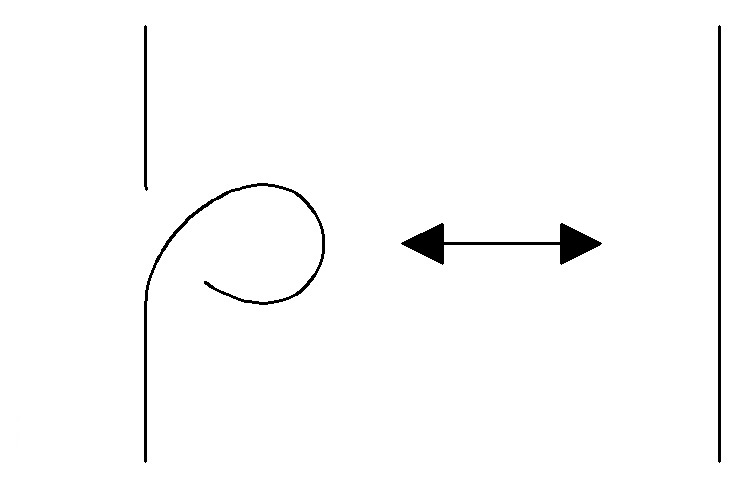
\includegraphics[scale=0.2]{1/pictures/R1}
		\end{center}
	\end{minipage}
\item Drugi ruch Reidemeistera: 

	\begin{minipage}{0.5\textwidth}
		\begin{center}
			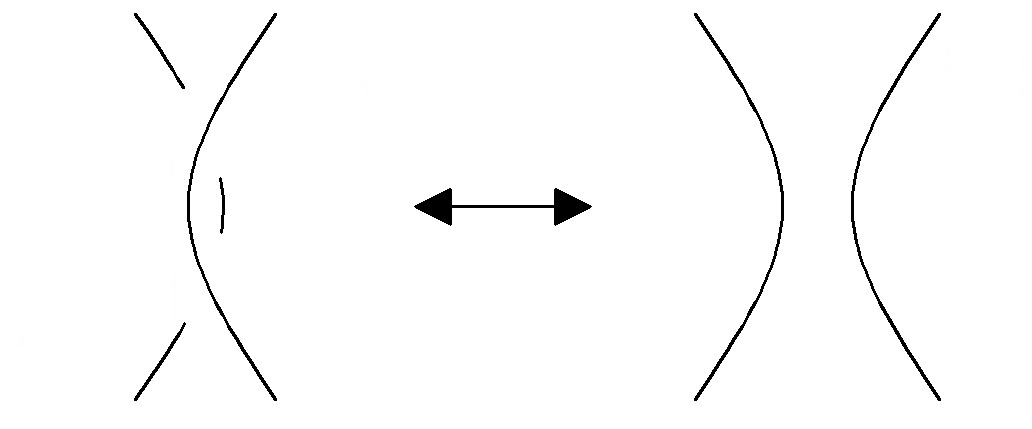
\includegraphics[scale=0.2]{1/pictures/R2}
		\end{center}
	\end{minipage}
	
\item Trzeci ruch Reidemeistera: 

	\begin{minipage}{0.65\textwidth}
		\begin{center}
			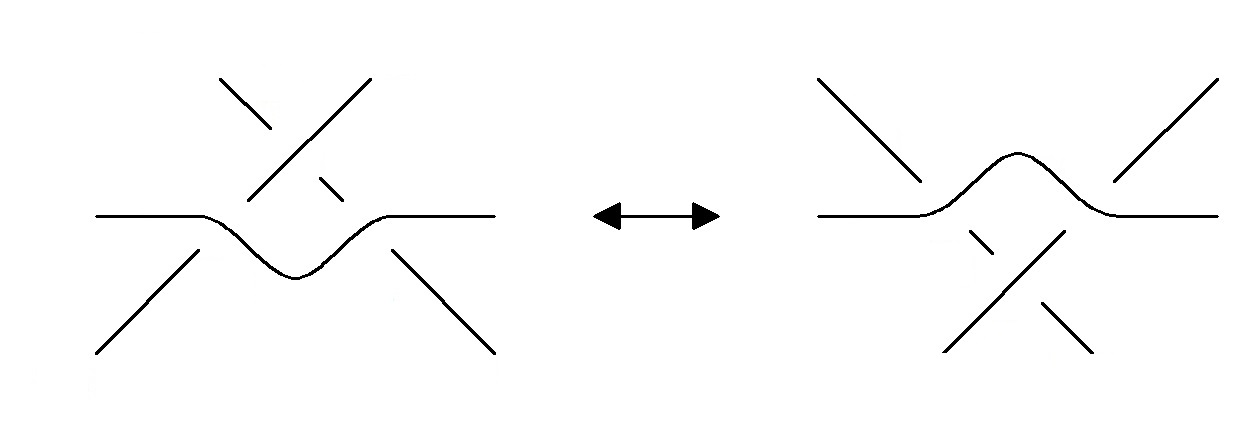
\includegraphics[scale=0.25]{1/pictures/R3}
		\end{center}
	\end{minipage}
	
	\end{enumerate}
 
\end{definicja}

\begin{definicja}
 Dwa diagramy uważa się za równoważne, gdy za pomocą skończonej liczby ruchów Reidemeistera z jednego diagramu można otrzymać drugi.
\end{definicja}

\begin{twierdzenie}{(Reidemeister'a)}
Dwa węzły są równoważne, wtedy i tylko wtedy, gdy ich diagramy są równoważne.
\end{twierdzenie}

\begin{proof}

Załóżmy najpierw, że mamy dane węzły $J$ i $K$, oba te węzły mają regularny rzut na płaszczyznę, oraz węzeł $K$ można otrzymać z węzła $J$ przez pewien ciąg elementarnych deformacji.
Ponieważ ten ciąg jest skończony, bez zmniejszenia ogólności możemy założyć, że węzeł $K$ powstaje z węzła $J$ w wyniku jednej elementarnej deformacji. Wystarczy więc pokazać, że 
ta deformacja odpowiada ciągowi ruchów R na diagramie węzła $J$. 

Rozważmy pojedynczą elementarną deformację węzła $J$ w sensie definicji \ref{wygoda}. Powiedzmy że $J = (v_1, \ldots, v_{i-1}, v_i, v_{i+1}, \ldots, v_n)$, oraz że 
$K = (v_1, \ldots, v_{i-1}, v', v_{i+1}, \ldots, v_n)$. Ogólny przypadek na pierwszy rzut wydaje się być mocno skomplikowany. Opiszemy go za pomocą wielu podprzypadków, z którymi
w prosty sposób potrafimy sobie poradzić. 

Niech $C$ oznacza czworokąt $v_{i-1}, v_i, v_{i+1}, v'$, przez $o$ oznaczmy odcinek $vv'$. Przez $S$ oznaczmy zbiór skrzyżowań z wnętrza $C$ (jako podzbiór $\mathbb{R}^2$), 
przez $W$ oznaczmy zbiór wierzchołków z wnętrza $C$, przez $P$ oznaczmy zbiór punktów przecięcia osi $o$ z łukami z wnętrza $C$. 
Oczywiście zbiór $S\cup W\cup P$ jest skończony. Niech $A$ oznacza obraz tego zbioru przez rzut promienisty na $o$, to znaczy, jeśli dany punkt $p$ jest po tej samej stronie osi $o$, 
co punkt $v_{i-1}$($v_{i+1}$), to rzutem promienistym punktu $p$ na $o$ nazwiemy rzutowanie na $o$ w kierunku prostej zawierającej odcinek $[p, v_{i-1}]$($[p, v_{i+1}]$). 
Możemy założyć, że rzuty punktów z $S\cup W\cup P$ są parami różne, oraz że żadne skrzyżowanie ani wierzchołek nie leżą na osi $o$.
Jeśli by tak nie było, możemy używając drugiego ruchu R odrobinę poprzesuwać skrzyżowania i miejsca przecięcia łuków z osią. 
Niestety w przypadku, kiedy skrzyżowanie i wierzchołek znajdują się na prostej, wzdłuż której odbywa się rzutowanie, sytuacja jest nieco bardziej skomplikowana, co widać na poniższym
rysunku.



	\begin{center}

	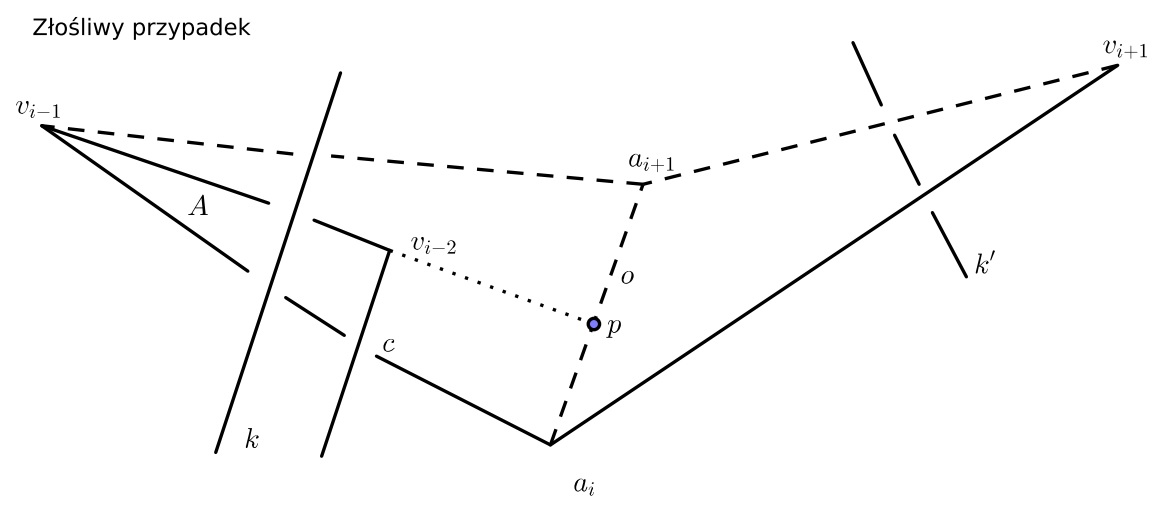
\includegraphics[scale=0.5]{1/pictures/bad.jpg}
	\end{center}


Oczywiście łuków złośliwych w sensie złośliwości łuku $k$ może być więcej, niż jeden (bez zmniejszenia ogólności możemy założyć, że wewnątrz $C$ nie ma skrzyżowań - 
to założenie będzie łatwo wynikać z dalszej części dowodu), ale będzie istniał taki, którego skrzyżowanie z $I_{i-1}$ będzie najbliżej wierzchołka $v_{i-2}$.
Radząc sobie z tym delikwentem, oraz używając indukcji (skończonej), jesteśmy w stanie poradzić sobie z przypadkiem, kiedy złośliwych łuków jest dowolnie wiele. To jednak nie wyczerpuje
wszystkich tego typu przypadków. Istnieje kilka podobnych (ale nie jest ich wiele, pamiętajmy, że $C$ ma być rozłączny z resztą węzła), np. łuk $k$ przechodzi pod czworokątem $C$, a odcinki $I_{i-2}, I_{i-1}$ przechodzą pod $k$. 
Ponieważ wszystkie te przypadki są bardzo podobne, tu opiszemy tylko jeden, a resztę zostawiamy czytelnikowi jako nietrudne ćwiczenie.
Aby poradzić sobie z przypadkiem przedstawionym na rysunku powyżej, należy najpierw łuk $k$ przenieść na drugą stronę skrzyżowania $c$ (trzeci ruch R), potem cofnąć wierzchołek $v_{i-2}$
tak, żeby znajdował się bliżej wierzchołka $v_{i-1}$ niż łuk $k$ przed przesunięciem (tu nam pomoże drugi ruch R zastosowany parokrotnie), 
następnie wrócić łuk $k$ na jego pierwotne miejsce (znów trzeci ruch R).
 

Niech $B$ oznacza zbiór zrzutowanych punktów na oś $o$. Wprowadżmy na $o$ następującą relację porządku: $x < y\iff d(v_i,x) < d(v_i, y)$. Ustawmy zbiór $B$ rosnąco $x_1, x_2, \ldots, x_{l-1}$.
Niech $v_i = a_0, a_1, a_2, \ldots, a_l = v'$ będzie ciągiem punktów, takim że $a_i\in o$, oraz $x_i < a_i < x_{i+1}$ w sensie wprowadzonego porządku. 
Wystarczy zatem pokazać, że każdą z elementarnych deformacji przeprowadzających wierzchołek $v_i$ na $a_1$, wierchołek $a_1$ na punkt $a_2$, $\ldots$, 
wierzchołek $a_{l-1}$ na punkt $a_l$ można uzyskać za pomocą sekwencji ruchów R, co prowadzi do rozbicia problemu na wiele mniejszych podprzypadków, których lista znajduje się
poniżej.


	\begin{center}

	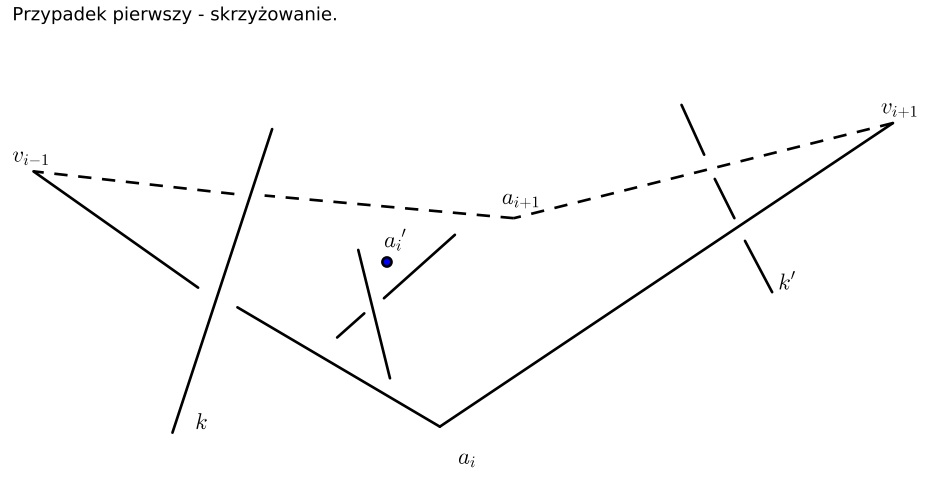
\includegraphics[scale=0.6]{1/pictures/cross.jpg}
	\end{center}

Łuki skrzyżowania mogą przechodzić, albo oba nad bokami czworokąta $C$, albo oba pod bokami $C$, albo jeden może leżeć nad czworokątem, a drugi pod. Dwa pierwsze przypadki są oczywiste,
radzimy sobie z nimi stosując trzeci ruch R, oraz w celach kosmetycznych drugi ruch R. Trzeci przypadek jest nieco trudniejszy, ale również główną rolę gra w nim trzeci ruch R. Po
prostu można przenieść łuk, który przechodzi nad czworokątem $C$ na drugą stronę skrzyżowania łuku przechodzącego pod czworokątem $C$ i łuku $a_i v_{i-1}$, potem parokrotnie zastosować
drugi ruch R a na koniec znów zastosować trzeci ruch R, żeby przenieść łuk, który ruszyliśmy na początku, na jego pierwotne miejsce.


	\begin{center}

	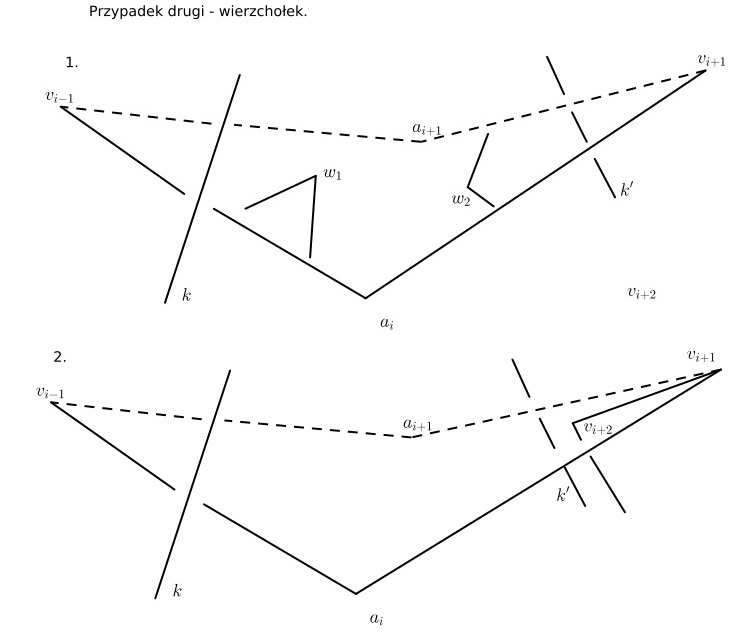
\includegraphics[scale=0.8]{1/pictures/vertex.jpg}
	\end{center}

	
Podprzypadek pierwszy jest prosty, wystarczy zastosować drugi ruch R. Przypadek drugi wymaga nieco komentarza. 

Żeby poradzić sobie z przypadkiem 2. należy zastosować pierwszy ruch R (wcześniej go nie stosowaliśmy) do pętli $a_iv_{i+1}v_{i+2}$. To nam pozwoli wyrzucić wierzchołek $v_{i+2}$ z 
czworokąta $C$. Mamy też pewność, że efektem ubocznym tego ruchu nie będą żadne nowe skrzyżowania, ani wierzchołki, ani łuki przecinające oś $o$, zatem będziemy w stanie przenieść 
wierzchołek $a_i$ na wierzchołek $a_{i+1}$. Na koniec, musimy wykonać operację odwrotną do tej, która wyrzuciła wierzchołek $v_{i+2}$ z czworokąta $C$, która sprawi, że $v_{i+2}$
wróci na swoje pierwotne miejsce.


	\begin{center}

	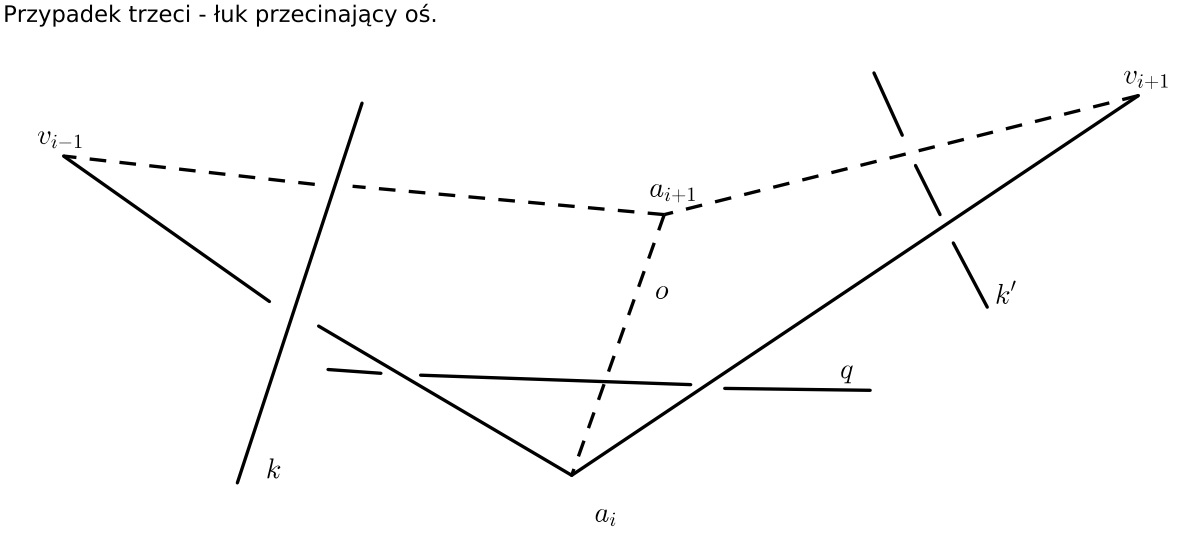
\includegraphics[scale=0.5]{1/pictures/axis.jpg}
	\end{center}

	
Ten przypadek jest prosty, żeby przenieść wierzchołek $a_i$ na drugą stronę łuku $q$ wystarczy zastosować drugi ruch R. Przypadek, kiedy łuk $q$ przechodzi nad czworokątem $C$ jest analogiczny.

Na koniec trzeba jeszcze pamiętać o naszym początkowym założeniu o tym, że rzuty są parami różne, i że żadne skrzyżowania, ani wierzchołki nie leżą na osi $o$. Jeśli potrzebowaliśmy
lekko zmodyfikować diagram wyjściowego węzła, żeby to założenie było prawdziwe, musimy na koniec wykonać modyfikacje odwrotne, które oczywiście można uzyskać za pomocą ruchów R.

W ten sposób zakończyliśmy szkic dowodu implikacji w jedną stronę. Implikacja w drugą stronę jest oczywista. 
	
\end{proof}

% Szymon
\section{Kolorowania węzłów}

 Głównym zadaniem teorii węzłów jest stworzenie narzędzi służących do opisywania, klasyfikowania oraz rozróżniania węzłów. Na podstawie twierdzenia przedstawionego w poprzedniej części wiemy że, diagramy są równoważne jeżeli pierwszy można przekształcić do drugiego stosując ruchy Reidemeistera. Sprawdzanie równoważności diagramów w ten sposób jest jednak uciążliwe, oraz czasochłonne.  W niniejszej części zostanie przedstawione zagadnienie kolorowania diagramów węzłów. Kolorowanie węzłów jest niezmiennikiem diagramu. Oznacza to że gdy pierwszy diagram posiada pewną własność kolorowania, a drugi nie, to diagramy te nie są równoważne, a więc przedstawiają różne węzły. Kolorowanie nie jest idealnym narzędziem klasyfikującym i istnieją diagramy nierównoważne o takich samych własnościach kolorowania. \\
 Kolejność omawianych zagadnień w tym rozdziale będzie następująca: Najpierw podana zostanie definicja kolorowania, oraz warunki które muszą zostać spełnione aby węzeł mógł zostać w określony sposób pokolorowany. Następnie zdefiniowane zostaną równania kolorowań oraz macierze kolorowań. Kolejnym etapem będzie wprowadzenie macierzy kolorowań jako niezmiennika węzłów. Ostatnią część stanowić będzie wskazanie relacji pomiędzy klasami diagramów węzłów a grupami kolorowań.

\subsection{Kolorowanie diagramów}

Niech K będzie węzłem zorientowanym, L jego diagramem, B = $\lbrace b_{1}, \ldots, b_{k}\rbrace$ zbiorem łuków,  C = $\lbrace c_{1}, \ldots, c_{k}\rbrace$ zbiorem skrzyżowań. 

\begin{definicja}
Diagram L jest kolorowalny modulo $n \in \N$, gdy każdemu łukowi diagramu L można przyporządkować liczbę $a \in \lbrace 0, \ldots, n-1 \rbrace$ w taki sposób, że: \\ \\
	\begin{minipage}{0.7\textwidth}
	
	\begin{enumerate}
		\item Dla każdego skrzyżowania $c_{j}$ spełnione jest równanie kolorowania \\ $a_{2}+a_{3}-2a_{1} \equiv 0$ mod n
		\item Kolorowanie nie jest stale, tzn istnieją łuki $b_{i}, b_{j}$ którym 			przyporządkowano różne liczby.
		 
	\end{enumerate}
	\end{minipage}
	\begin{minipage}{0.3\textwidth}
	\begin{center}

	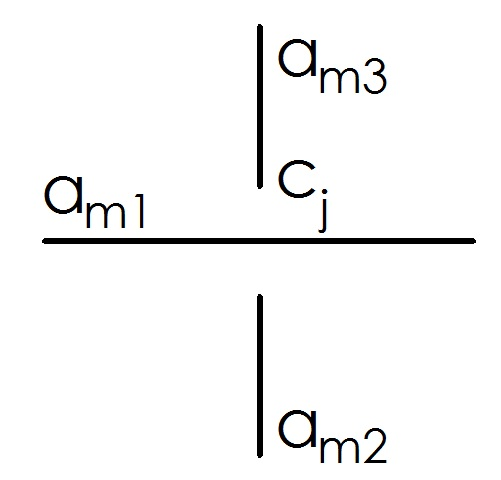
\includegraphics[scale=0.35]{2/Obrazy/Crossing1}
	\end{center}
	\end{minipage}
\end{definicja}
Przyporządkowanie spełniające powyższe własności nazywa się \emph{kolorowaniem diagramu mod n}.




\begin{twierdzenie} Kolorowalność modulo n jest niezmiennikiem węzła.
\end{twierdzenie}
\begin{proof}
Dwa diagramy $L_{1}, L_{2}$ są równoważne jeżeli istnieje ciąg ruchów Reidemeistera przekształcający $L_{1}$ w $L_{2}$. Wystarczy zatem sprawdzić że kolorowalność modulo n nie zmienia się po wpływem ruchów Reidemeistera.

\begin{enumerate} \item Pierwszy ruch Reidemeistera: 

	\begin{minipage}{0.5\textwidth}
	Dla skrzyżowania $c_{j}$ spełnione jest równanie \\ $a_{1}+a_{2}-2a_{2} \equiv 0$ mod n. Zatem $a_{1} \equiv a_{2}$.
	\end{minipage}
	\begin{minipage}{0.5\textwidth}
		\begin{center}
			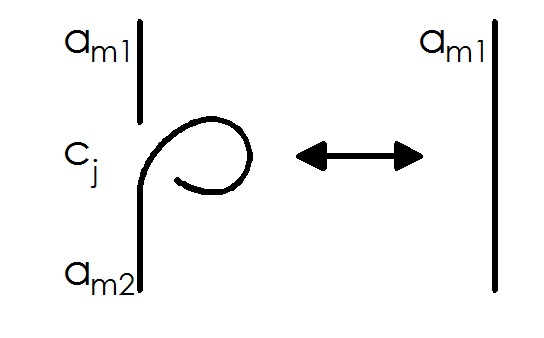
\includegraphics[scale=0.2]{2/Obrazy/R1}
		\end{center}
	\end{minipage}
\item Drugi ruch Reidemeistera: 

	\begin{minipage}{0.5\textwidth}
	Dla skrzyżowania $c_{j1}$ mamy \\ $a_{1}+a_{4}-2a_{2} \equiv 0$ mod n.\\ Dla skrzyżowania $c_{j2}$, \\$a_{3}+a_{4}-2a_{2} \equiv 0$ mod n. \\Stąd $a_{1} \equiv a_{3} $ mod n.
	\end{minipage}
	\begin{minipage}{0.5\textwidth}
		\begin{center}
			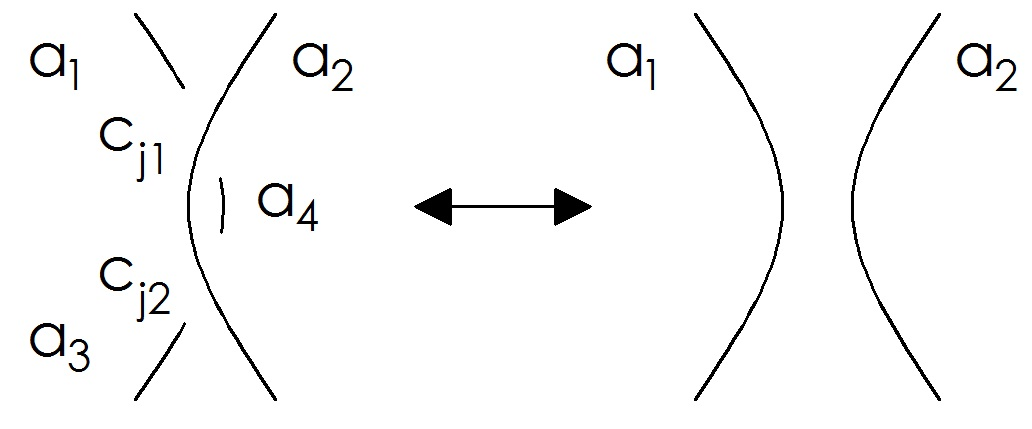
\includegraphics[scale=0.2]{2/Obrazy/R2}
		\end{center}
	\end{minipage}
	
\item Trzeci ruch Reidemeistera: 


	Dla skrzyżowania $c_{j2}$ mamy $a_{5}+a_{2}-2a_{3} \equiv 0$ mod n. Analogicznie dla skrzyżowania $c_{j5}$, $a_{8}+a_{2}-2a_{3} \equiv 0$ mod n. Stąd $a_{8} \equiv a_{5}$ mod n. \\ \\
	\begin{minipage}{0.35\textwidth}
	W drugim przypadku mamy:\\
	$a_{4} \equiv 2a_{2}-a_{1}$. \\
	$a_{6} \equiv 2a_{3}-a_{4} \equiv$ \\$\equiv 2a_{3}-2a_{2}+a_{1} $.	\\
	$a_{8} \equiv 2a_{3}-a_{2}$. \\	
	$a_{7} \equiv 2a_{3}-a_{1}$.\\		
	$a_{9} \equiv 2a_{8}-a_{7} \equiv$ \\$\equiv 2a_{3}-2a_{2}+a_{1} \equiv a_{6} $. \\
	\end{minipage}
	\begin{minipage}{0.65\textwidth}
		\begin{center}
			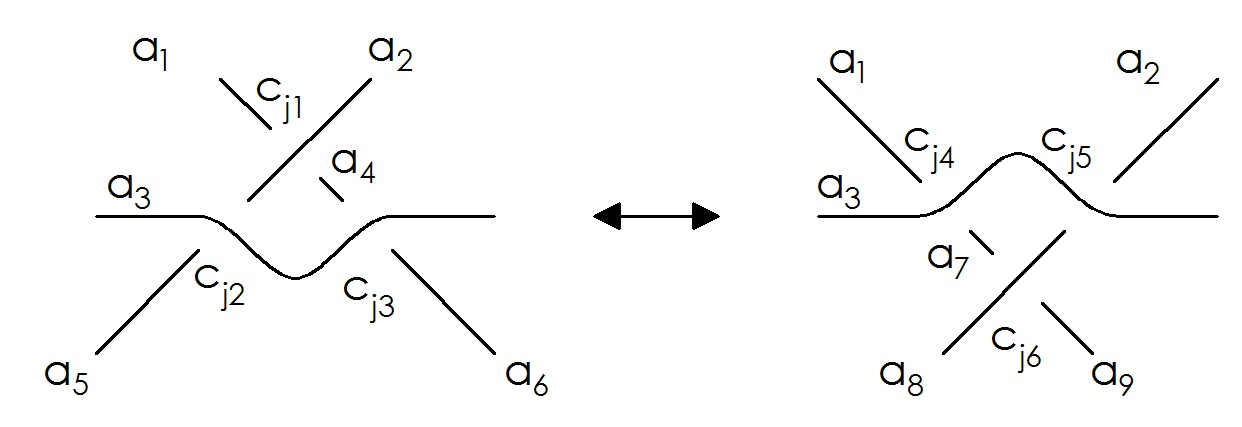
\includegraphics[scale=0.25]{2/Obrazy/R3}
		\end{center}
	\end{minipage}
	Zatem, kolory łuków o indeksach różnych od 7 nie ulegają zmianie. Kolor łuku $a_{7}$ zmienia się i wynosi $a_{7} \equiv a_{6} - a_{2} + a_{4}$. W otrzymane kolorowanie spełnia równania kolorowań w diagramie $L_{2}$.
\end{enumerate}
\end{proof}


\begin{definicja}
Niech B = $\lbrace b_{1}, \ldots, b_{k}\rbrace$ będzie zbiorem łuków. Kolorowaniem $(a_{b_{1}}, \ldots, a_{b_{k}})$ nazywamy przyporządkowanie każdemu łukowi $b_{i}$ koloru $a_{b{i}}$, tak aby spełnione były równania kolorowań. W dalszej części opracowania zapis ten zostanie uproszczony do postaci $(a_{1}, \ldots, a_{k})$, gdzie indeks przy $a$, odpowiada numerowi łuku, którego ten kolor dotyczy.
\end{definicja}


\begin{lemat}
Jeżeli dla diagramu L istnieje kolorowanie $( a_{1}, \ldots , a_{k} )$, to dla każdego l $\in \N\:\: ( a_{1}+l, \ldots , a_{k}+l )$ też jest kolorowaniem.
\end{lemat}
\begin{proof}
Dla każdego $c_{j}$ spełnione jest:\\
$a_{m_{1}}+a_{m_{2}}-2a_{m_{3}} \equiv 0$ mod n. Wobec czego \\ 
$a_{m_{1}}+l+a_{m_{2}}+l-2a_{m_{3}}-2l \equiv 0$.
\end{proof}
\textbf{Wniosek:} Jeśli diagram jest kolorowalny to istnieje kolorowanie takie że $a_{1} = 0$.

\paragraph{Kolorowanie modulo 2} Jeżeli węzeł jest kolorowalny modulo 2 to dla każdego skrzyżowania zachodzi jedna z czterech możliwości:
	\begin{center}
			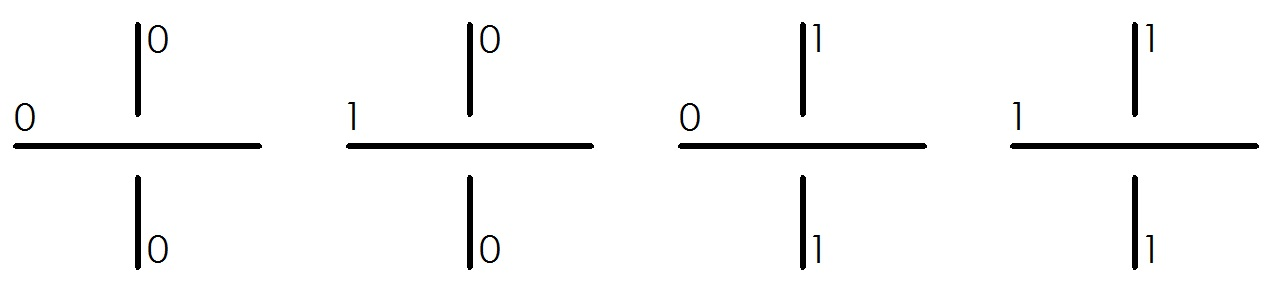
\includegraphics[scale=0.3]{2/Obrazy/Mod2}
	\end{center}
	W każdym przypadku kolory łuków leżących po przeciwnych stronach skrzyżowania są jednakowe. Startując w dowolnym punkcie węzłą i przechodząc go w wybranym kierunku otrzymamy że każdy łuk należący do tej samej komponenty spójności co punkt startowy ma przyporządkowany jednakowy kolor. Zatem splot może być kolorowany mod 2 $\Leftrightarrow$ splot składa się z co najmniej 2 węzłów.
	
	\begin{definicja}
	Niech K będzie splotem, L jego diagramem. Diagram L jest podzielny jeśli splot składa się z co najmniej 2 węzłów, oraz  $\exists U, V\:  otwarte, U \cap V = \emptyset$, takie że $ L\subseteq U\cup V, L\cap U \neq \emptyset, L\cap V \neq \emptyset$.
	\end{definicja}
	
	
\begin{lemat}
	Jeżeli splot K jest podzielny to, $\forall n >1 \:\:$ diagram L jest kolorowalny mod n.
\end{lemat}
	
\begin{proof}
Niech każdy łuk zawarty w U będzie pokolorowany na kolor 0, łuk zawarty w V na kolor 1. Takie przyporządkowanie jest kolorowaniem. Równania skrzyżowań zachodzą dla każdego n. 
\end{proof}


	
\subsection{Równania kolorowań}
\begin{definicja}
Krótki łuk, to część łuku który przechodzi dokładnie przez 2 skrzyżowania. 
\end{definicja}
Przykład: Łuk $b_{1}$ przechodzi przez 5 skrzyżowań i składa się z 4 krótkich łuków. \\

\begin{center}
			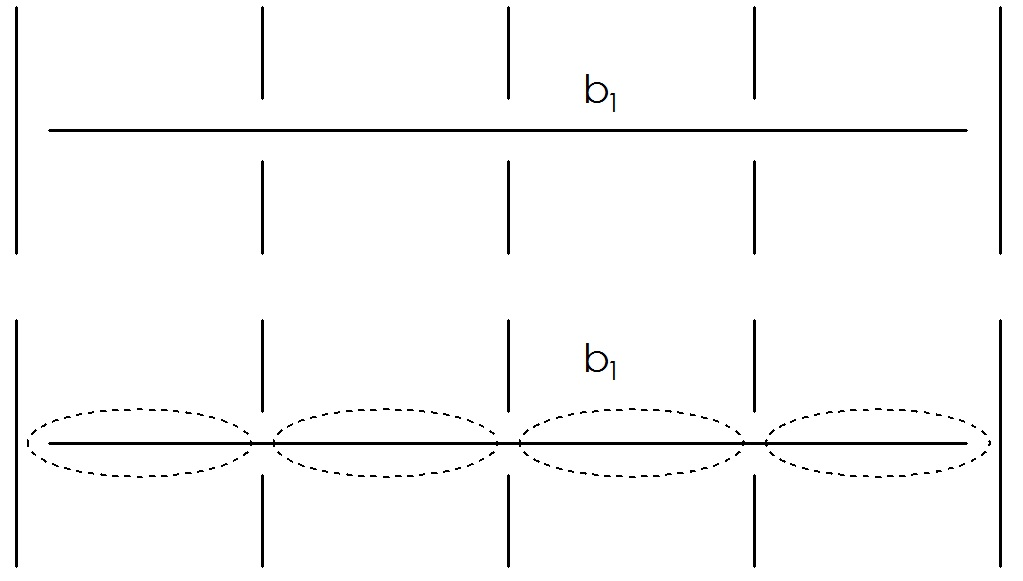
\includegraphics[scale=0.2]{2/Obrazy/ShortArc} \\
\end{center}

\begin{definicja}
Region to komponenta spójności $\R^{2} \setminus L$.
\end{definicja}
\begin{definicja}
Szachownica diagramu to przyporządkowanie każdemu regionowi jednego z 2 kolorów tak aby każdy krótki łuk oddzielał regiony o różnych kolorach.
\end{definicja}

\textbf{Przykład:} Rozważmy węzeł który w literaturze jest oznaczony symbolem $7_{3}$. Diagram węzła jest przedstawiony na rysunku poniżej (pierwszy z lewej). Węzeł posiada 7 łuków, 14 krótkich łuków, oraz 9 regionów.

			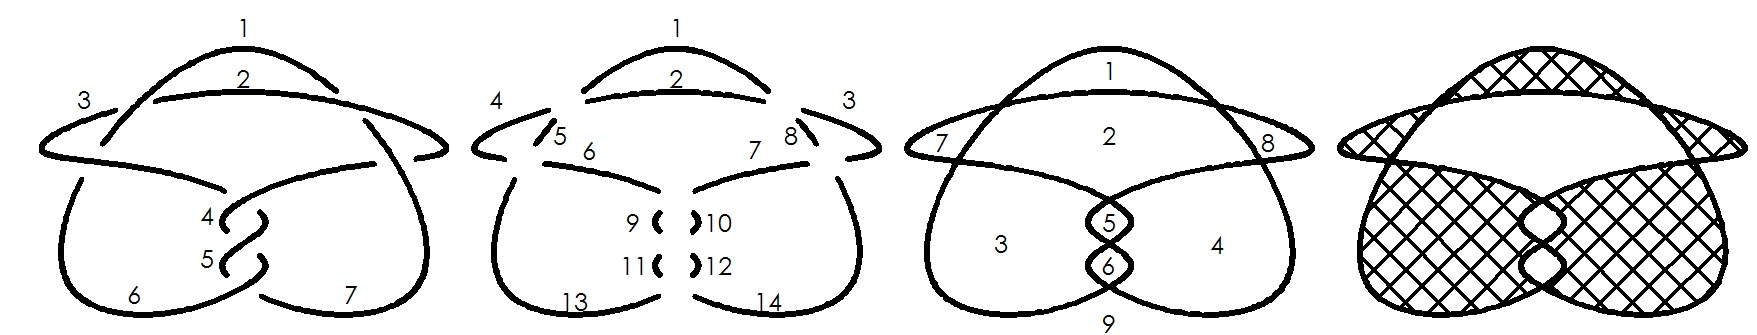
\includegraphics[scale=0.3]{2/Obrazy/ArcRegion3} \\



\begin{lemat}
Dla każdego węzła K istnieje szachownica jego diagramu.  
\end{lemat}
\begin{proof}
Ustalmy węzeł K, oraz jego diagram L. Niech $L$ będzie zawarty w pewnej kuli otwartej $\Omega$.
Weźmy dowolny region diagramu L. Ustalmy punkt P należący do tego regionu. Weźmy dowolne dwie krzywe o następujących własnościach:




	\begin{minipage}{0.5\textwidth}
\begin{itemize}
\item Krzywe są bez samo przecięć i nie przecinają się wzajemnie,
\item Początki krzywych znajdują się w punkcie P,
\item Końce krzywych znajdują się na brzegu $\Omega$,
\item Krzywa nie przechodzi przez skrzyżowania.	
\end{itemize}
	\end{minipage}
	\begin{minipage}{0.5\textwidth}
		\begin{center}
			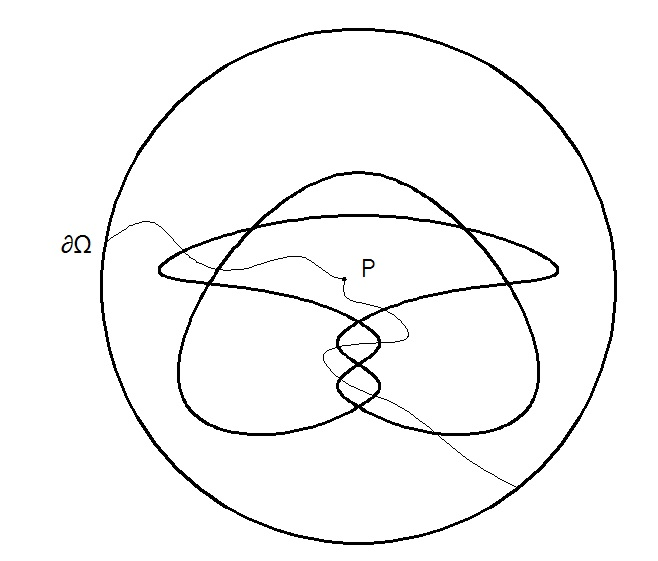
\includegraphics[scale=0.3]{2/Obrazy/Chesscircle}
		\end{center}
	\end{minipage}
Zatem suma krzywych dzieli węzeł na 2 części. Ponadto obie krzywe przecinają parzystą liczbę łuków. Zatem każda z krzywych przecina taką samą liczbę łuków modulo 2. Stąd kolor regionu nie zależy od wyboru krzywej, więc szachownica diagramu istnieje zawsze. 

\end{proof}
Dla każdego skrzyżowania $c_{j}$ równanie można przedstawić na 2 sposoby. 

\begin{definicja}
Wybór znaku równania kolorowania nazywa się dobrym, gdy przyjmuje następującą postać: 
\end{definicja}

	\begin{minipage}{0.5\textwidth}
$a_{m2}+a_{m3}-2a_{m1} \equiv 0$ mod n, dla \\	
	\begin{center}
			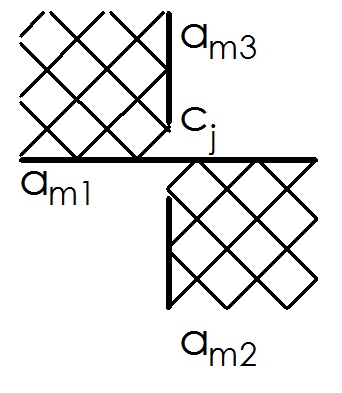
\includegraphics[scale=0.3]{2/Obrazy/Cros+}
	\end{center}
	\end{minipage}
	\begin{minipage}{0.5\textwidth}
$2a_{m1}-a_{m2}-a_{m3} \equiv 0$ mod n, dla \\
	\begin{center}
			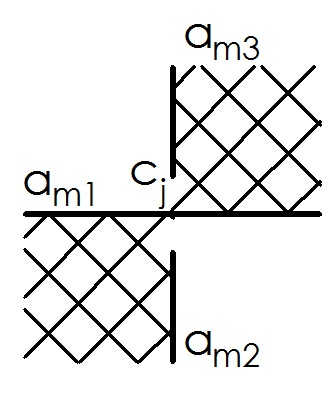
\includegraphics[scale=0.3]{2/Obrazy/Cros-}
	\end{center}	
	\end{minipage}

\begin{lemat}
Suma równań po wszystkich skrzyżowaniach równa się 0, o ile znaki równań zostały \emph{wybrane dobrze}.
\end{lemat}
\begin{proof}
Ustalmy dowolny łuk $b_{j}$, z kolorem  $a_{j}$. Łuk $b_{j}$ składa się z pewnej liczby krótkich łuków $b_{j}^{i}$. Każdy krótki łuk łączy dokładnie 2 skrzyżowania. Istnieje region $X_{i}$, taki że oba skrzyżowania graniczą z $X_{i}$. Niech $a_{j}^{i}$ oznacza kolor $b_{j}^{i}$ krótkiego łuku. Kolor każdego krótkiego łuku występuje w równaniach dokładnie 2 skrzyżowań.
\begin{center}
  			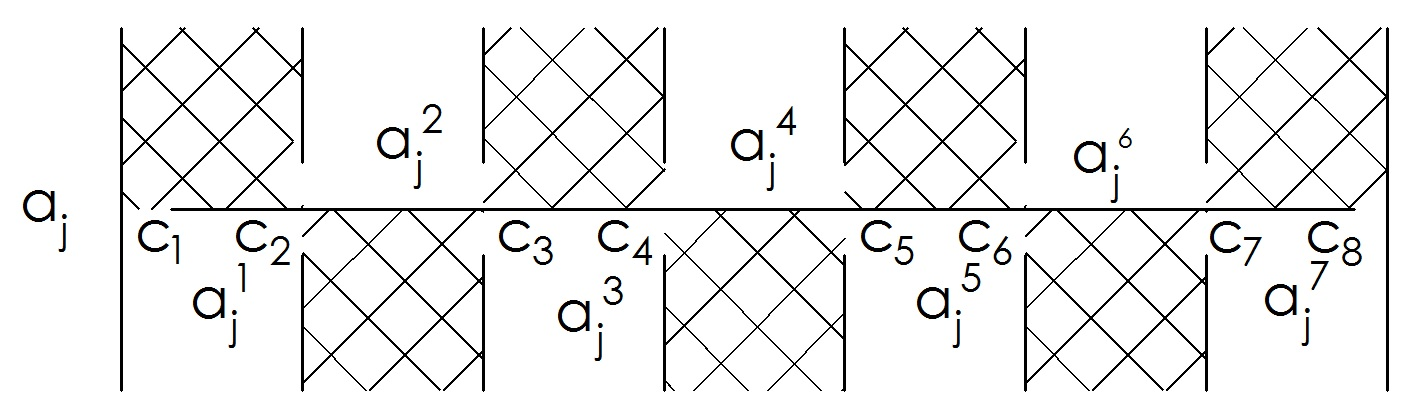
\includegraphics[scale=0.3]{2/Obrazy/zerosum2}
\end{center}
Ponieważ znaki równań zostały  \emph{wybrane dobrze}, znak $a_{j}^{i}$ w równaniu skrzyżowania  
$c_{j1}$, jest przeciwny do znaku $a_{j}^{i}$ w równaniu skrzyżowania $c_{j2}$. Wobec czego równania dla krótkich łuków sumują się do 0, dla każdego i. Zatem sumują się również do 0 dla równań kolorowań zwykłych łuków.
\end{proof}

\textbf{Wniosek:} Niech łuk j, ma początek w skrzyżowaniu $c_{m}$. Zaczynając w $c_{m}$ a następnie idąc wzdłuż łuku i sumując współczynniki przy j-tym łuku w mijanych równaniach skrzyżowań, suma zawsze wynosi $\pm 1$.
\begin{proof}
Zamiast sumować współczynniki przy j-tym łuku w kolejnych równaniach skrzyżowań można sumować współczynniki przy odpowiadających mu krótkich łukach. Z lematu współczynniki sumują się do 0. Zatem suma wszystkich współczynników jest równa współczynnikowi krótkiego łuku przy ostatnim mijanym skrzyżowaniu, a ten współczynnik wynosi $\pm 1$.

\end{proof}

\begin{comment}
\begin{lemat}
Dla każdego  każdego łuku j można tak wybrać znaki dla każdego skrzyżowania dla każdego skrzyżowania, że suma równań po wszystkich skrzyżowaniach równa się 0, oraz suma współczynników przy łuku j po skrzyżowaniach ze zbioru W równa się $\pm 1$.
\end{lemat}

\begin{proof}

\end{proof}
\end{comment}

\subsection{Macierze kolorowań}
\begin{definicja}
Łuk zamknięty w diagramie to węzeł składający się dokładnie z jednego łuku.
\end{definicja}
\begin{center}
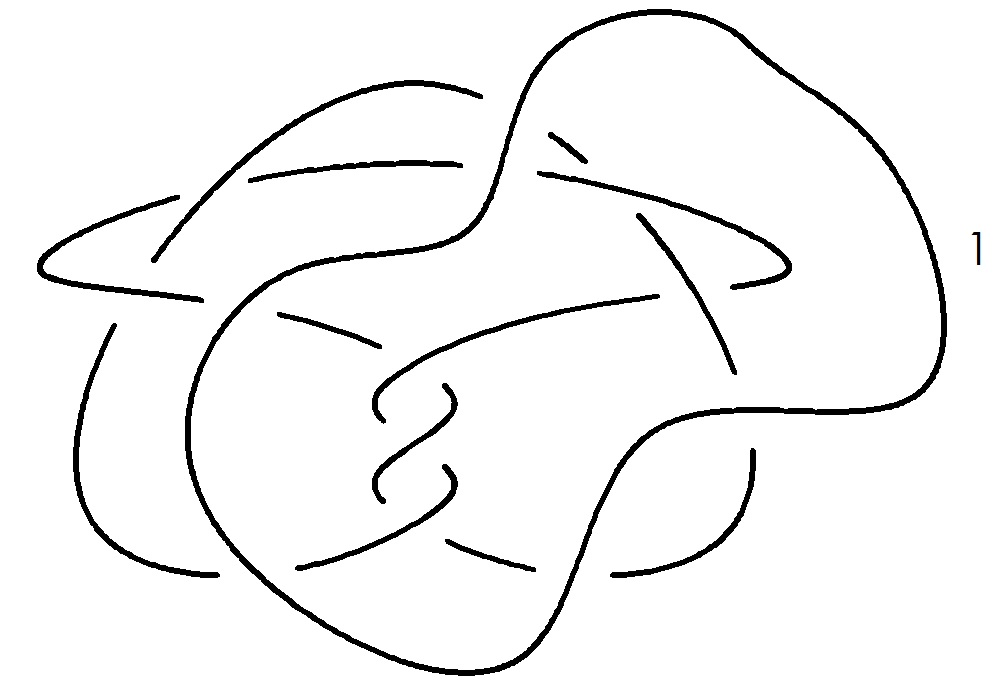
\includegraphics[scale=0.2]{2/Obrazy/Clossedcurve} \\

\end{center}

\begin{lemat}
Jeżeli węzeł K nie zawiera łuków zamkniętych, to liczba skrzyżowań i łuków w diagramie L jest równa .
\end{lemat}
\begin{proof}
Niech L będzie diagramem zorientowanym. Ponieważ węzeł nie zawiera łuków zamkniętych to dla każdego łuku istnieją dokładnie 2 skrzyżowania które odpowiadają początkowi i końcowi łuku. Dodatkowo każde skrzyżowanie jest początkiem i końcem dokładnie 2 łuków. Zatem funkcja przyporządkowywująca łukowi skrzyżowanie będące jego początkiem jest bijekcją.
\end{proof}


Niech L będzie diagramem bez łuków zamkniętych, B zbiorem łuków, $( a_{1}, \ldots, a_{k})$ jego kolorowaniem modulo n, C zbiorem skrzyżowań.  
\begin{definicja}
Macierz kolorowania $A_{+}$ to macierz powstała ze współczynników występujących w równaniach kolorowań diagramu L, przy czym znaki równań kolorowań zostały wybrane dobrze. $A_{+}=(a_{ij})$, gdzie  $a_{ij}$ odpowiada współczynnikowi przy kolorze i-tego łuku w równaniu $c_{j}$-tego skrzyżowania. 
\end{definicja}
Proces tworzenia macierzy $A_{+}$, dla węzła $7_{3}$ został przedstawiony poniżej. \\

	\begin{minipage}{0.5\textwidth}

	\begin{center}
			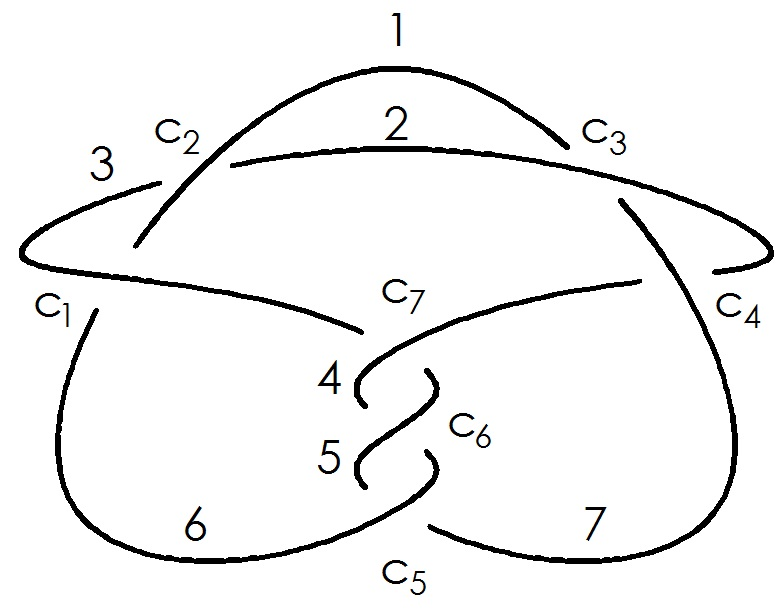
\includegraphics[scale=0.3]{2/Obrazy/73matrix}
	\end{center}
	\end{minipage}
	\begin{minipage}{0.5\textwidth}

	\begin{center}
			$c_{1}: \quad a_{1} + a_{6} - 2a_{3} \equiv 0 $ mod n
			$c_{2}: \quad a_{2} + a_{3} - 2a_{1} \equiv 0 $ mod n
			$c_{3}: \quad a_{1} + a_{7} - 2a_{2} \equiv 0 $ mod n	
			$c_{4}: \quad a_{2} + a_{4} - 2a_{7} \equiv 0 $ mod n	
			$c_{5}: \quad a_{5} + a_{7} - 2a_{6} \equiv 0 $ mod n	
			$c_{6}: \quad a_{4} + a_{6} - 2a_{5} \equiv 0 $ mod n	
			$c_{7}: \quad a_{3} + a_{5} - 2a_{4} \equiv 0 $ mod n	
	\end{center}	
	\end{minipage}
	
\begin{center}


$\newline A_{+} = \bordermatrix { ~ & 1 & 2 & 3 & 4 & 5 & 6 & 7  \cr
					c_{1} & 1 & 0 &-2 & 0 & 0 & 1 & 0	 \cr
					c_{2} &-2 & 1 & 1 & 0 & 0 & 0 & 0  \cr
					c_{3} & 1 &-2 & 0 & 0 & 0 & 0 & 1  \cr
					c_{4} & 0 & 1 & 0 & 1 & 0 & 0 &-2  \cr
					c_{5} & 0 & 0 & 0 & 0 & 1 &-2 & 1  \cr
					c_{6} & 0 & 0 & 0 & 1 &-2 & 1 & 0  \cr
					c_{7} & 0 & 0 & 1 &-2 & 1 & 0 & 0  \cr} $

\end{center}
$\newline$
\textbf{Obserwacja:} Równania kolorowań diagramu L są liniowo zależne, bo sumują się do 0. Zatem wyznacznik macierzy kolorowania $\vert det  \big(A_{+}\big) \vert = 0$.
  
  \begin{definicja}
	Macierz kolorowań $A$ wymiaru $(k-1) \times (k-1)$, to dowolny minor macierzy $A_{+}$ powstały poprzez usunięcie jednego wiersza i jednej kolumny.
  \end{definicja}
    \begin{definicja}
    Wyznacznik diagramu $ det \big(L\big)$ to moduł z wyznacznika $\vert det \big(A\big) \vert$.
    \end{definicja}
    
\begin{twierdzenie}
Wyznacznik diagramu jest dobrze określony, nie zależy od wyboru minora macierzy $A_{+}$
\end{twierdzenie}

\begin{proof}
Niech $A_{i,j}$ oznacza minor powstały poprzez usunięcie i-tego wiersza, oraz j-tej kolumny. W macierzy $A_{+}$ suma elementów w wierszu, oraz suma elementów w kolumnie równa się 0, ponieważ znaki równań są wybrane dobrze. Niech X będzie macierzą $k \times k$, oraz X = 
$
\begin{pmatrix}
 1 & \cdots & 1 \\
 \vdots & \ddots & \vdots \\
 1 & \cdots & 1 \\
\end{pmatrix}
$. Rozważmy \\
\begin{center}
 $det\big( A_{+}+X \big)=det \begin{pmatrix}
 1+a_{1,1} & \cdots & 1+a_{1,k} \\
 \vdots & \ddots & \vdots \\
 1+a_{k,1} & \cdots & 1+a_{k,k} \\
\end{pmatrix}$ \\
\end{center} 
Suma elementów w każdej kolumnie, oraz w każdym wierszu równa się k. Wyznacznik zostanie obliczony w następujących krokach:
\begin{enumerate}
\item Po dodaniu do  i-tego wiersza, sumy pozostałych wierszy każdy element i-tego wiersza będzie mieć wartość k. Wartości w pozostałych komórkach pozostaną niezmienione. \\
\begin{center}

$det \begin{pmatrix}
 1+a_{1,1} & \cdots &  1+a_{1,k} \\
 \vdots & \ddots & \vdots \\
  k & \cdots &  k \\ 
 \vdots & \ddots & \vdots \\
 1+a_{k,1} & \cdots & 1+a_{k,k} \\
\end{pmatrix}$ \\
\end{center}

\item Po dodaniu do j-tej kolumny, sumy pozostałych kolumn, element $a_{i,j}$ będzie mieć wartość $k^2$. Pozostałe elementy w i-tym wierszu, oraz j-tej kolumnie będą mieć wartość k. Pozostałe elementy pozostaną niezmienione. \\
\begin{center}
$det \begin{pmatrix}
 1+a_{1,1} & \cdots & k & \cdots &  1+a_{1,k} \\
 \vdots & \ddots & \vdots & \ddots & \vdots \\
  k & \cdots & k^2 & \cdots & k \\ 
 \vdots & \ddots & \vdots & \ddots & \vdots \\
 1+a_{k,1} & \cdots & k & \cdots &  1+a_{k,k} \\
\end{pmatrix}$ \\
\end{center}

\item Po wyciągnięciu k przed wyznacznik, wyrażenie będzie miało postać. \\
\begin{center}
$k \times det \begin{pmatrix}
 1+a_{1,1} & \cdots & k & \cdots &  1+a_{1,k} \\
 \vdots & \ddots & \vdots & \ddots & \vdots \\
  1 & \cdots & k & \cdots & 1 \\ 
 \vdots & \ddots & \vdots & \ddots & \vdots \\
 1+a_{k,1} & \cdots & k & \cdots &  1+a_{k,k} \\
\end{pmatrix}$ \\
\end{center}
\item Odejmując i-ty wiersz od pozostałych wierszy otrzymamy. 
\begin{center}
$k \times det \begin{pmatrix}
 a_{1,1} & \cdots & 0 & \cdots &  a_{1,k} \\
 \vdots & \ddots & \vdots & \ddots & \vdots \\
  1 & \cdots & k & \cdots & 1 \\ 
 \vdots & \ddots & \vdots & \ddots & \vdots \\
 a_{k,1} & \cdots & 0 & \cdots &  a_{k,k} \\
\end{pmatrix}$ \\
\end{center}

Korzystając z rozwinięcia Lalpace'a względem j-tej kolumny: \\ $\vert det  \big(A+X \big) \vert = k^2 \times \vert (-1)^{i+j} \times det \big( A_{i,j} \big) \vert$, dla każdego $i, j$. Zatem $\vert det \big( A_{i,j} \big) \vert$ nie zależy do wyboru $i, j$. 

\end{enumerate}


\end{proof}



\subsection{Własności wyznacznika diagramu}
Wyznacznik diagramu jest powiązany z możliwymi kolorowaniami diagramu.

\begin{lemat}
Niech A będzie macierzą o wyrazach całkowitych. Istnieją macierze X, Y o wyrazach całkowitych, takie że $\vert det(X) \vert= \vert det(Y) \vert=1$, oraz macierz diagonalna $\vert D \vert=(\vert d_{i,i} \vert)$, jedyna z dokładnością do permutacji wyrazów na głównej przekątnej, takie że $D=XAY$.
\end{lemat}
\begin{proof}
Niech A będzie macierzą wymiaru $k \times k$, oraz  $a$ liczbą całkowitą. Ustalmy macierze:
\begin{itemize}
\item $Z^1_{i,j}$  -  Macierz odpowiadająca transpozycji i-tej, oraz j-tego wektora macierzy A,

\item $Z^2_{i,aj}$ -  Macierz odpowiadająca dodaniu do  i-tego wektora, a-tą krotność j-tego wektora.
\end{itemize}
Każda z powyższych macierzy ma wyznacznik 1. \\
$\textbf{Krok 1:}$ Mnożąc macierz $A$ z lewej lub prawej przez $Z^1$ da się 
ją przekształcić do postaci $A^{(1)}$, takiej że najmniejszy co do modułu, niezerowy wyraz znajduje się w lewym górnym rogu macierzy. Następnie mnożąc z lewej lub prawej przez 
$Z^2_{i,a1}$, można przekształcić macierz do postaci $A^{(2)}$ takiej że, wartość bezwzględna każdego elementu leżącego w pierwszym wierszu lub pierwszej kolumnie jest mniejsza od wartości bezwzględnej elementu $a_{1,1}$. \\
$\textbf{Krok 2:}$ Powtarzając Krok 1, można sprowadzić macierz do postaci 
\begin{center}
$A^{(n_{1})}=\begin{pmatrix}
a_{1,1} & 0 & \cdots & 0 \\
0 & a_{2,2} & \cdots & a_{2,k} \\
\vdots & \ddots & \ddots & \vdots \\
0 & a_{k,2} & \cdots & a_{k,k} \\
\end{pmatrix}$
\end{center}
$\textbf{Krok 3:}$ Powtarzając krok 1 i 2 dla macierzy wymiaru $(k-1) \times (k-1)$ otrzyma się macierz 
\begin{center}
$A^{(n_{2})}=\begin{pmatrix}
a_{1,1} & 0 & 0 & \cdots & 0 \\
0 & a_{2,2} & 0 & \cdots & 0 \\
0 & 0 & a_{3,3} & \cdots & a_{3,k} \\
\vdots & \vdots & \vdots & \ddots  & \vdots \\
0 & 0 & a_{k,3} & \cdots & a_{k,k} \\
\end{pmatrix}$ \\
\end{center}
$\textbf{Krok 4:}$ Indukcyjnie, macierz A może zostać sprowadzona do postaci diagonalnej D. Operacje wykonywane na kolumnach odpowiadają mnożeniu macierzy A przez $Z^i$ z prawej strony, na wierszach przez mnożenie z lewej strony. Zatem macierze X, Y są postaci: \\

	\begin{minipage}{0.5\textwidth}
	\begin{center}
	
 $X=\prod_{m} Z^m$.
 
	\end{center}
	\end{minipage}
	\begin{minipage}{0.5\textwidth}
	\begin{center}
	
$Y=\prod_{n} Z^n$.

	\end{center}	
	\end{minipage}
$\newline$
$Z^m, Z^n \in \lbrace Z^1_{i(m),j(m)}, Z^2_{i(m),aj(m)} \rbrace$,odpowiadają kolejno wykonywanym operacjom wierszowym i kolumnowym. Ponieważ $\vert det(Z^i) \vert=1 \Rightarrow \vert det(D) \vert= \vert \prod^k_{i=1} d_{k} \vert = \vert det(XAY) \vert = \vert det(A) \vert$, 


\end{proof}

\begin{twierdzenie}
Wyznacznik diagramu L, oraz wartości w odpowiadającej mu macierzy diagonalnej są niezmiennikiem węzła.
\end{twierdzenie}
\begin{proof}
Niech K będzie węzłem, L jego diagramem, B = $\lbrace b_{1}, \ldots, b_{k}\rbrace$ zbiorem łuków,  C zbiorem skrzyżowań, $\lbrace a_{1}, \ldots, a_{k}\rbrace$ jego kolorowaniem modulo n, $A_{+}$ macierzą kolorowania, $A$ minorem $A_{+}$, powstałym po usunięciu k-tego wiersza i k-tej kolumny. Wystarczy sprawdzić że wyznacznik diagramu oraz struktura macierzy diagonalnej nie zmienia się pod wpływem ruchów Reidemeistera.  
\begin{enumerate}
\item Pierwszy ruch Reidemeistera. Bez straty ogólności można założyć że ruch Reidemeistera jest przeprowadzany na k-tym łuku, pomiędzy i, oraz i+1 skrzyżowaniem. Dodatkowo można przyjąć że indeksy skrzyżowań do których dochodzi łuk k są mniejsze od i+1, oraz indeksy skrzyżowań do których dochodzi k+1, są większe od i. W rezultacie,  macierz $A'_{+}$  po transformacji, ma wymiar $k+1$. Elementy o obu indeksach mniejszych  od $k$ pozostają niezmienione.

\begin{minipage}{0.5\textwidth}
\begin{center}
			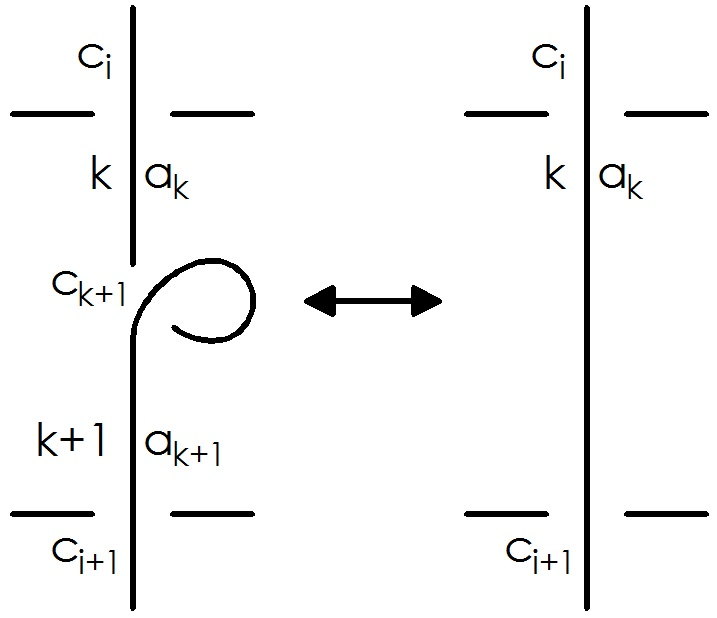
\includegraphics[scale=0.25]{2/Obrazy/R1det}
\end{center}
\end{minipage}
\begin{minipage}{0.5\textwidth}
\begin{center}

			$A'_{+}= \begin{pmatrix}
			${\Huge A}$ & \begin{matrix} a_{1,k} \\ \vdots \\ a_{i,k} \\ 0 \\ \vdots
			\\ 0 \end{matrix} & \begin{matrix} 0 \\ \vdots \\ 0 \\ a_{i+1,k} \\ \vdots
			\\ a_{k-1,k} \end{matrix} \\
			\begin{matrix} a_{k,1} & \cdots & a_{k,k-1} \end{matrix} & 0 & a_{k,k} \\
			\begin{matrix} 0 & \cdots & 0 \end{matrix} & -1 & 1 \\
			\end{pmatrix}$

			
\end{center}
\end{minipage}



\begin{comment}

			$A'_{+}= \begin{pmatrix}
			${\Huge A}$ & \begin{matrix} 0 \\ \vdots \\ 0 \\ 0 \\ \vdots
			\\ 0 \end{matrix} & \begin{matrix} 0 \\ \vdots \\ 0 \\ 0 \\ \vdots
			\\ 0 \end{matrix} \\
			\begin{matrix} 0 & \cdots & 0 \end{matrix} & 0 & 0 \\
			\begin{matrix} 0 & \cdots & 0 \end{matrix} & -1 & 1 \\
			\end{pmatrix}$
\end{comment}

Równania skrzyżowań o indeksach od 1 do i nie zmieniają się. W równaniach skrzyżowań o indeksach większych od i, k-ty kolor zostaje zastąpiony k+1-szym. Ostatni wiersz macierzy wynika z równania $c_{k+1}$ skrzyżowania. Na mocy lematu znaki równań mogą być tak dobrane aby sumowały się one do 0. Co więcej taki dobór znaków jest również właściwy dla macierzy $A_{+}$. Niech $A'$ będzie minorem $A'_{+}$ powstałym poprzez usunięcie ostatniej kolumny i ostatniego wiersza. 

\begin{center}

			$\newline
			\newline
			\newline
			A'= \begin{pmatrix}
			${\Huge A}$ & \begin{matrix} a_{1,k} \\ \vdots \\ a_{i,k} \\ 0 \\ \vdots
			\\ 0 \end{matrix} \\
			\begin{matrix} a_{k,1} & \cdots & a_{k,k-1} \end{matrix} & 0 \\
			\end{pmatrix}$
			
\end{center}

Dodając do k-tego wiersza sumę pozostałych wierszy otrzymamy macierz:
\begin{center}

			$\begin{pmatrix}
			${\Huge A}$ & \begin{matrix} a_{1,k} \\ \vdots \\ a_{i,k} \\ 0 \\ \vdots
			\\ 0 \end{matrix} \\
			\begin{matrix} 0 & \cdots & 0 \end{matrix} & 1 \\
			\end{pmatrix}$
			
\end{center}


Stąd korzystając z rozwinięcia Laplace'a względem ostatniego wiersza, $\vert det \big(A'\big) \vert = \vert 1 \times det \big(A\big) \vert$. Przenosząc element $a_{k,k} =1$ w lewy górny róg macierzy i powtarzając rozumowanie z twierdzenia o postaci macierzy diagonalnej, otrzymujemy, że jeśli macierz diagonalna odpowiadająca $A$ ma wartości na głównej przekątnej $\lbrace \vert d_{1} \vert, \cdots, \vert d_{k-1} \vert \rbrace$, to macierz diagonalna odpowiadająca $A'$, ma wartości $\lbrace 1, \vert d_{1} \vert, \cdots, \vert d_{k-1} \vert \rbrace$

\item Drugi ruch Reidemeistera. Bez straty ogólności można założyć że ruch Reidemeistera dotyczy i-tego, oraz k-tego łuku, gdzie i-ty łuk jest łukiem górnym, oraz ruch jest pomiędzy  skrzyżowaniami $ c_{j}, c_{j+1}$. 

\begin{center}
			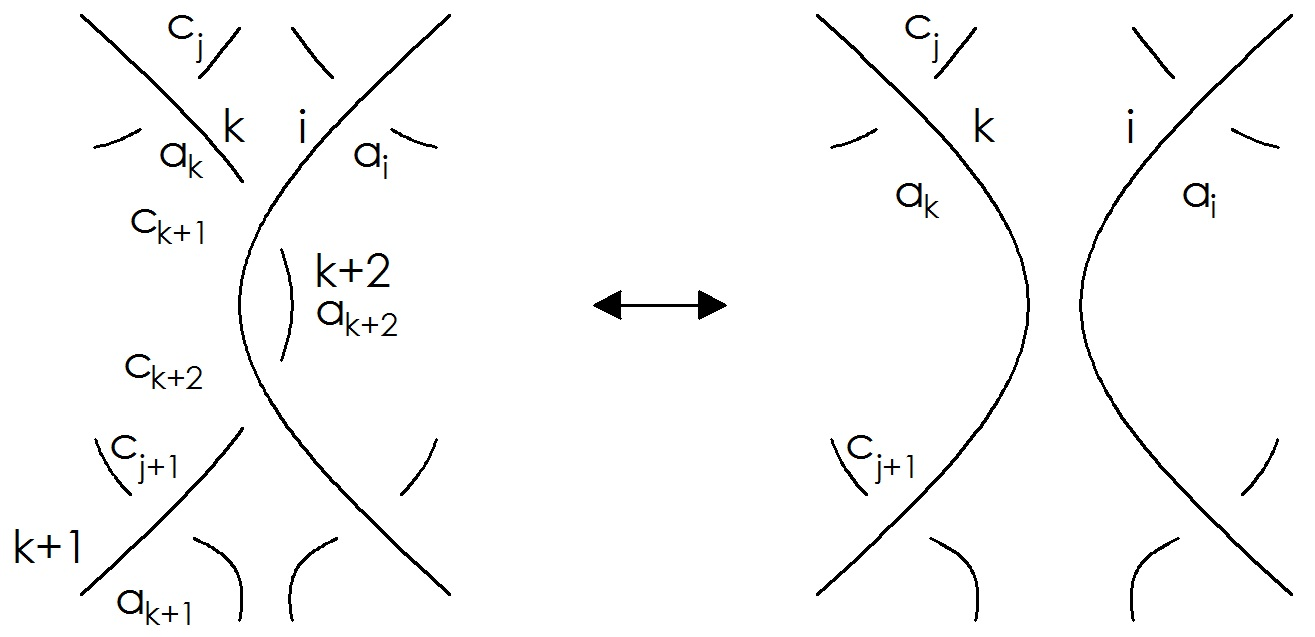
\includegraphics[scale=0.25]{2/Obrazy/R2det}
\end{center}

Niech indeksy skrzyżowań do których dochodzi łuk k są mniejsze od i+1, oraz indeksy skrzyżowań do których dochodzi k+1, są większe od i. Równania skrzyżowań do których nie dochodzi łuk $k+1$ nie zmieniają się. Macierze kolorowania mają zatem postacie:

\begin{center}

			$A'_{+}= \begin{pmatrix}
			${\Huge A}$ & \begin{matrix} a_{1,k} \\ \vdots \\ a_{i,k} \\ 0 \\ \vdots
			\\ 0 \end{matrix} & \begin{matrix} 0 \\ \vdots \\ 0 \\ a_{i+1,k} \\ \vdots
			\\ a_{k-1,k} \end{matrix} & \begin{matrix} 0 \\ \vdots \\ 0 \\ 0 \\ \vdots
			\\ 0 \end{matrix} \\
	 		\\ \begin{matrix} a_{k,1} & \cdots  & a_{k,i}  & \cdots & a_{k,k-1} \end{matrix} & 0 & a_{k,k} & 0
	 		\\ \begin{matrix} 0 & \cdots & 0 & -2 & 0 & \cdots & 0 \end{matrix} & 1 & 0 & 1
			\\ \begin{matrix} 0 & \cdots & 0 & 2 & 0 & \cdots & 0 \end{matrix} & 0 & -1 & -1

			\end{pmatrix}$

	
\end{center}

\begin{center}

			$A'= \begin{pmatrix}
			${\Huge A}$ & \begin{matrix} a_{1,k} \\ \vdots \\ a_{i,k} \\ 0 \\ \vdots
			\\ 0 \end{matrix} & \begin{matrix} 0 \\ \vdots \\ 0 \\ a_{i+1,k} \\ \vdots
			\\ a_{k-1,k} \end{matrix}
	 		\\ \begin{matrix} a_{k,1} & \cdots  & a_{k,i}  & \cdots & a_{k,k-1} \end{matrix} & 0 & a_{k,k}
	 		\\ \begin{matrix} 0 & \cdots & 0 & -2 & 0 & \cdots & 0 \end{matrix} & 1 & 0 


			\end{pmatrix}$

		
\end{center}

Po wykonaniu na macierzy $A'$ następujących operacji: dodanie do ostatniej (k+1) kolumny sumy pozostałych kolumn, oraz dodanie do przedostatniego wiersza (k) sumy wierszy od 1 do k-1, oraz zastosowaniu rozwinięcia Laplace'a otrzymamy $\vert det \big( A' \big) \vert = \vert det \big( A \big) \vert$. Macierz diagonalna ma postać $\lbrace 1, 1, \vert d_{1} \vert, \cdots, \vert d_{k} \vert \rbrace$. Argumentacja jest analogiczna jak w pierwszym ruchu Reidemeistera.
 
 \item Trzeci ruch Reidemeistera. Trzeci ruch nie zmienia liczby skrzyżowań. Macierze $A_{+}$, oraz $A'_{+}$ mają wymiar $k \times k$. Bez straty ogólności można przyjąć 

\end{enumerate}
\end{proof}



\begin{twierdzenie}
Diagram L może być kolorowalny mod n $\Leftrightarrow \vert det(L) \vert$ oraz n nie są względnie pierwsze.

\end{twierdzenie}

\begin{proof}
Istnienie kolorowania mod n oznacza istnienie kolorów $\lbrace a_{1}, \cdots, a_{k} \rbrace$, takich że równania kolorowań są spełnione dla każdego skrzyżowania. Równoważnie, jest spełnione równanie macierzowe: $ A_{+}x \equiv 0$ mod n, $x \in \Z^k_{n}$. Z lematu wynika, że można przyjąć $a_{1} = 0 $. Ponieważ równania kolorowań są liniowo zależne i $a_{1} = 0 $, zatem powyższa równość zachodzi $\Leftrightarrow Ax' \equiv 0$ mod n, $x' \in \Z^{k-1}_{n}$. \\
Korzystając z twierdzenia o postaci diagonalnej otrzymujemy $A = X^{-1} D Y^{-1}$. \\ $X^{-1}$, $Y^{-1}$ są macierzami całkowitoliczbowymi. Niech $\overline{X^{-1}} = X^{-1}$ mod n, $\overline{Y^{-1}} = Y^{-1}$ mod n, oznacza przypisanie każdemu elementowi macierzy, reszty z dzielenia mod n. Stąd $Ax' \equiv 0 \Leftrightarrow \overline{A}x' \equiv 0 \Leftrightarrow \overline{X^{-1} D Y^{-1}}x' \equiv 0 \Leftrightarrow \overline{X^{-1}} \times \overline{D} \times \overline{Y^{-1}}x' \equiv 0 \Leftrightarrow \overline{D} y' \equiv 0$, $y' =Y^{-1}x'$, $y' \in \Z^{k-1}_{n}$. Ponieważ kolorowanie $x'$ nie jest trywialne, to $y' \neq 0$ mod n. Zatem $\exists i \in \lbrace 1, \cdots, k \rbrace$  $d_{i} \times y'_{i} \neq 0$ mod n. Ponieważ $\forall i \in \lbrace 1, \cdots, k \rbrace$  $y'_{i} \in \Z_{n}$, to $d_{i}$, oraz $n$, nie są względnie pierwsze. Ponadto $\vert det \big(L \big) \vert =\vert det \big(D \big) \vert= \prod^k_{i=1} \vert d_{i}\vert$. Stąd $det \big(L \big)$, oraz $n$ nie są względnie pierwsze.
\end{proof}
\textbf{Wniosek:} 
\begin{itemize}
\item Jeżeli $\vert det \big(L \big) \vert = 0$, to dla każdego n, diagram jest kolorowalny modulo n,
\item Jeżeli $\vert det \big(L \big) \vert = 1$, to dla żadnego n, diagram nie jest. kolorowalny modulo n
\end{itemize}


\subsection{Wyznacznik sumy spójnej} 
Niech $K$, $\tilde{K}$ będą węzłami, $L$, $\tilde{L}$ ich diagramami, $A_{+}$, $\tilde{A_{+}}$ macierzami kolorowania, $C$, $\tilde{C}$ zbiorami skrzyżowań. Rozważmy sumę spójną węzłów $K\#\tilde{K}$. Bez straty ogólności można przyjąć dwa upraszczające założenia:
\begin{itemize}
\item Diagramy zostały połączone względem k-tego łuku w diagramie $L$, oraz względem pierwszego łuku w diagramie $\tilde{L}$.  
\item Skrzyżowania w diagramie $L$ zostały tak ponumerowane że skrzyżowania do których dochodzi łuk k, oraz znajdują się przed miejscem połączenia diagramów mają numer mniejszy od i+1, zaś skrzyżowania znajdujące się za miejscem połączenia mają numer większy od i. Analogicznie dla diagramu $\tilde{L}$. 
\end{itemize} 

\begin{twierdzenie}
Wyznacznik sumy spójnej diagramów $\vert det \big( K\#\tilde{K} \big) \vert = \vert det \big( K \big) \vert \times \vert det \big( \tilde{K} \big) \vert$. Ponadto jeżeli wartości w odpowiadających macierzach diagonalnych wynoszą $\lbrace \vert d_{1} \vert, \cdots, \vert d_{k} \vert \rbrace$, oraz $\lbrace \vert \tilde {  d_{1}} \vert , \cdots,  \vert\tilde{ d_{k}} \vert \rbrace$, to wartości w macierzy diagonalnej dla diagramu sumy spójnej wynoszą $\lbrace 1, \vert d_{1}, \cdots, \vert d_{k}, \vert \tilde {d_{1}} \vert, \cdots, \vert \tilde{d_{k}} \vert\rbrace$.
\end{twierdzenie}

\begin{proof}
Operacja sumy spójnej przerywa dwa wybrane łuki i łączy końce. 
\begin{center}
			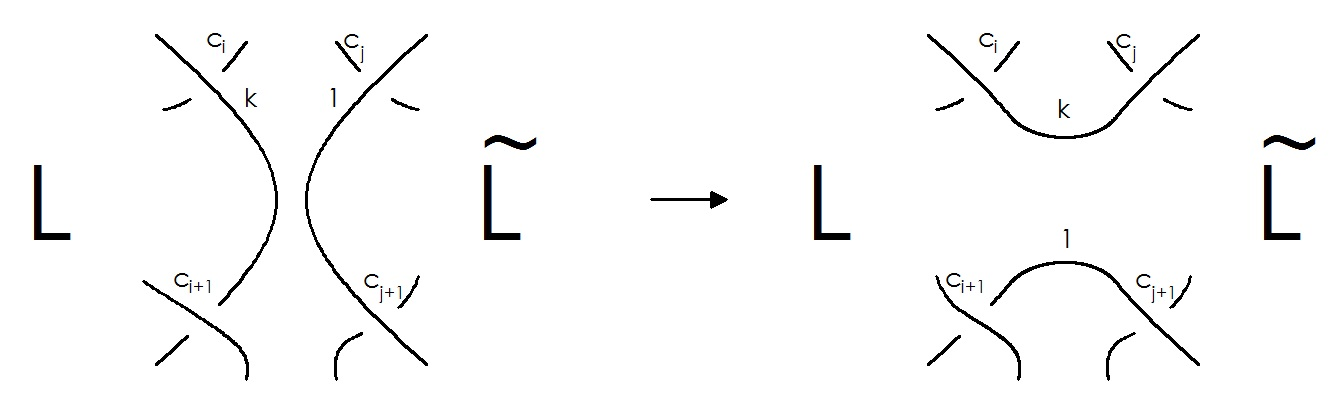
\includegraphics[scale=0.3]{2/Obrazy/Sumaspojna}
\end{center}

W diagramie $L$, równania skrzyżowań o indeksach większych od i zostaną zmienione. Współczynnik odpowiadający łukowi k, będzie odpowiadał łukowi pierwszemu z diagramu $\tilde{L}$. W diagramie $\tilde{L}$, współczynnik odpowiadający łukowi pierwszemu będzie odpowiadał łukowi k z diagramu $L$. Macierz kolorowania ma postać: \\
\begin{center}

$\big( A_{L\#\tilde{L}}\big)_{+}= \begin{pmatrix} 

\begin{matrix}
a_{1,1} & \cdots & a_{1,k-1} \\
\vdots & \ddots & \vdots \\
a_{i,1} & \cdots & a_{i,k-1} \\
a_{i+1,1} & \cdots & a_{i+1,k-1} \\
\vdots & \ddots & \vdots \\
a_{k,1} & \cdots & a_{k,k-1} \\
\end{matrix}

&
\begin{matrix}
a_{1,k}\\
\vdots\\
a_{i,k}\\
0\\
\vdots\\
0
\end{matrix}
&
\begin{matrix}
0\\
\vdots\\
0\\
a_{i+1,k}\\
\vdots\\
a_{k,k}

\end{matrix}
&
${\Huge{0}}$


\\
${\Huge{0}}$
&
\begin{matrix}
\tilde{a}_{1,1}\\
\vdots\\
\tilde{a}_{\tilde{i},1}\\
0\\
\vdots\\
0
\end{matrix}
&
\begin{matrix}
0\\
\vdots\\
0\\
\tilde{a}_{\tilde{i}+1,1}\\
\vdots\\
\tilde{a}_{k,1}

\end{matrix}
&
\begin{matrix}
\tilde{a}_{1,2} & \cdots & \tilde{a}_{1,k} \\
\vdots & \ddots & \vdots \\
\tilde{a}_{\tilde{i},2} & \cdots & \tilde{a}_{\tilde{i},k} \\
\tilde{a}_{\tilde{i}+1,2} & \cdots & \tilde{a}_{\tilde{i}+1,k} \\
\vdots & \ddots & \vdots \\
\tilde{a}_{k,2} & \cdots & \tilde{a}_{k,k} \\
\end{matrix}

\end{pmatrix}$
\end{center}
Po usunięciu z macierzy k+1-szego wiersza oraz k+1-szej kolumny otrzymamy 
\begin{center}

$ A_{L\#\tilde{L}}= \begin{pmatrix} 

\begin{matrix}
a_{1,1} & \cdots & a_{1,k-1} \\
\vdots & \ddots & \vdots \\
a_{i,1} & \cdots & a_{i,k-1} \\
a_{i+1,1} & \cdots & a_{i+1,k-1} \\
\vdots & \ddots & \vdots \\
a_{k,1} & \cdots & a_{k,k-1} \\
\end{matrix}

&
\begin{matrix}
a_{1,k}\\
\vdots\\
a_{i,k}\\
0\\
\vdots\\
0
\end{matrix}

&
${\Huge{0}}$


\\
${\Huge{0}}$
&
\begin{matrix}
\tilde{a}_{2,1}\\
\vdots\\
\tilde{a}_{\tilde{i},1}\\
0\\
\vdots\\
0
\end{matrix}

&
\begin{matrix}
\tilde{a}_{2,2} & \cdots & \tilde{a}_{2,k} \\
\vdots & \ddots & \vdots \\
\tilde{a}_{\tilde{i},2} & \cdots & \tilde{a}_{\tilde{i},k} \\
\tilde{a}_{\tilde{i}+1,2} & \cdots & \tilde{a}_{\tilde{i}+1,k} \\
\vdots & \ddots & \vdots \\
\tilde{a}_{k,2} & \cdots & \tilde{a}_{k,k} \\
\end{matrix}

\end{pmatrix}$
\end{center}
Następnie dodając do $k$-tego wiersza sumę wierszy od $1$ do $k-1$, oraz zamieniając $k$-ty wiersz z $k+\tilde{k}$-szym wierszem i $k$-tą kolumnę z $k+\tilde{k}$ kolumną mamy:


\begin{center}

$ A_{L\#\tilde{L}}= \begin{pmatrix} ${\Huge{A}}$ & ${\Huge{0}}$ &
\begin{matrix}
0\\
\vdots\\
0
\end{matrix} \\

${\Huge{0}}$ & ${\Huge{$\tilde{A}$}}$ & \begin{matrix}
0\\
\vdots\\
0
\end{matrix}  \\

\begin{matrix}
0 & \cdots & 0
\end{matrix} 
&
\begin{matrix}
0 & \cdots & 0
\end{matrix} 
&
\sum_{m=1}^i a_{m,k}

\end{pmatrix}
   $ 
    
\end{center}

Na podstawie wniosku o szachownicy diagramu $\sum_{m=1}^i a_{m,k}=\mp 1$. Zatem $\vert det \big(A_{L\#\tilde{L}} \big) \vert = 1 \times \vert det \big(A_{L} \big) \vert \times \vert det \big(A_{\tilde{L}} \big) \vert$. 
Ponadto przesuwając 1 w lewy górny róg macierzy i stosując proces diagonalizacji otrzymamy, że elementami macierzy diagonalnej są $\lbrace 1, \vert d_{1} \vert, \cdots, \vert d_{k} \vert,  \vert \tilde {d_{1}} \vert, \cdots, \vert \tilde{d_{k}}  \vert \rbrace$.

\end{proof}



\subsection{Grupy kolorowań}
\begin{definicja}
Grupa kolorowań diagramu Col(L), to grupa abelowa, w której generatorami są łuki diagramu, zaś relacjami są równania kolorowań, oraz ustalony koloru wybranego łuku, $a_{1} = 0$.\\ Formalnie: $Col(L)=\langle a_{1}, \cdots, a_{k} \big\vert \begin{pmatrix}
a_{j_{1}} + a_{j_{2}} - 2\times a_{j_{3}} \equiv 0 \\
\vdots \\
a_{j_{k-2}} + a_{j_{k-1}} - 2\times a_{j_{k}} \equiv 0
\end{pmatrix}, a_{1} = 0 \rangle$. \\
$Col(L) = \langle x \big\vert Ax \equiv 0 \rangle$, $x \in \Z^{k-1}$ \\
\end{definicja}

Grupa kolorowań nie jest dobrze zdefiniowanym pojęciem. Zależy ona bowiem od sposobu indeksowania łuków, skrzyżowań oraz wyboru koloru dla pierwszego elementu. 

\begin{twierdzenie}
Skończenie generowana grupa przemienna jest izomorficzna z produktem grup cyklicznych.
\end{twierdzenie}
Grupa kolorowań ma zatem postać: $Col(L) \cong \prod_{i=1}^m \Z_{n_{i}}$. \\
Z definicji grupy wynika że $Col(L) \cong \Z^m/\big(A\Z^m\big)$. Niech $A=X^{-1}DY^{-1}$ \\
$\Z^m/\big(A\Z^m\big) \cong \Z^m/\big(X^{-1}DY^{-1}\Z^m\big)  \cong \Z^m/\big(D\Z^m\big) \cong \Z^m/\big(\prod_{i=1}^m \vert d_{i} \vert \Z\big) \cong \prod_{i=1}^m \Z_{\vert d_{i} \vert}$ 

Klasa izomorfizmów grupy jest dobrze zdefiniowana. Wyznacznik, oraz wartości w macierzy diagonalnej nie zależą od wyboru diagramu, sposobu indeksowania łuków ani skrzyżowań. Produkt grup cyklicznych izomorficzny z grupą kolorowania jest niezmiennikiem węzła. \\
\textbf{Wniosek:} Grupa kolorowań jest nieskończona $\Leftrightarrow$ $det(\big(L\big) = 0$.


\subsection{Przykład zastosowań - rodzina węzłów}
\textbf{Przykład 1:}
Rozważmy następującą rodzinę węzłów $K_{k}$, $k \geq 3 $. Korzystając z własności kolorowań wykażemy że dla różnych k, diagramy przedstawiają różne węzły. 
\begin{center}
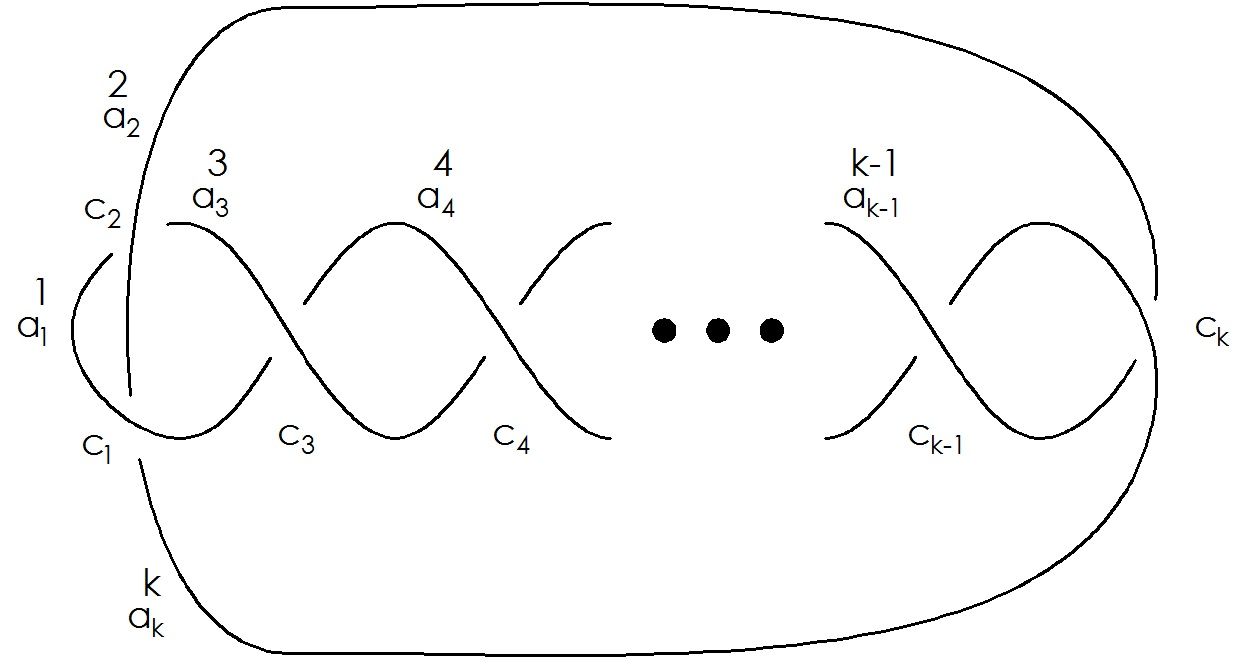
\includegraphics[scale=0.3]{2/Obrazy/Wezelprzyklad} \\
\end{center}
Macierz kolorowania ma postać:
\begin{center}


$A_{k+}=\bordermatrix{
~       &  1 &  2 &  3 &  4 &  5 & \cdots & k-2  &  k-1 &  k \cr
c_{1}   &  2 & -1 &  0 &  0 &  0 & \cdots &  0   &  0   & -1 \cr
c_{2}   & -1 &  2 & -1 &  0 &  0 & \cdots &  0   &  0   &  0 \cr
c_{3}   & -1 &  0 &  2 & -1 &  0 & \cdots &  0   &  0   &  0 \cr
c_{4}   &  0 &  0 & -1 &  2 & -1 & \cdots &  0   &  0   &  0 \cr
c_{5}   &  0 &  0 &  0 & -1 &  2 & \cdots &  0   &  0   &  0 \cr
\vdots  &  \vdots &  \vdots &  \vdots &  \vdots &  \vdots & \ddots &  \vdots   & \vdots   &  \vdots \cr
c_{k-2} &  0 &  0 &  0 &  0 &  0 & \cdots &  2   & -1   &  0 \cr
c_{k-1} &  0 &  0 &  0 &  0 &  0 & \cdots &  -1  &  2   & -1 \cr
c_{k}   &  0 & -1 &  0 &  0 &  0 & \cdots &  0   & -1   &  2 \cr}
$


\end{center}

Rozważmy macierz A, powstałą po usunięciu ostatniej kolumny i ostatniego wiersza. Za pomocą operacji wierszowych i kolumnowych, macierz zostanie sprowadzona do postaci diagonalnej.
\begin{center}

$A_{k}=\begin{pmatrix}
2  & -1 &  0 & 0 & 0 & 0 & \cdots & 0 & 0 & 0 \\
-1 &  2 & -1 & 0 & 0 & 0 & \cdots & 0 & 0 & 0 \\
-1 &  0 &  2 &-1 & 0 & 0 & \cdots & 0 & 0 & 0 \\
 0 &  0 & -1 & 2 &-1 & 0 & \cdots & 0 & 0 & 0 \\
 0 &  0 &  0 &-1 & 2 &-1 & \cdots & 0 & 0 & 0 \\
 \vdots  &  \vdots &  \vdots &  \vdots &  \vdots &  \vdots & \ddots &  \vdots   & \vdots   &  \vdots\\
 0 &  0 &  0 & 0 & 0 & 0 & \cdots &-1 & 2 &-1 \\
 0 &  0 &  0 & 0 & 0 &0  & \cdots & 0 &-1 & 2 \\
\end{pmatrix}$

\end{center}
Dodając do pierwszej kolumny, podwojoną drugą kolumnę, zamieniając pierwszą i drugą kolumnę miejscami, oraz dodając do drugiego wiersza podwojony pierwszy wiersz otrzymujemy. 
 \begin{center}
 

$A_{k}^{1} = \begin{pmatrix}
-1 &  0 &  0 & 0 & 0 & 0 & \cdots & 0 & 0 & 0 \\
 0 &  3 & -1 & 0 & 0 & 0 & \cdots & 0 & 0 & 0 \\
 0 & -1 &  2 &-1 & 0 & 0 & \cdots & 0 & 0 & 0 \\
 0 &  0 & -1 & 2 &-1 & 0 & \cdots & 0 & 0 & 0 \\
 0 &  0 &  0 &-1 & 2 &-1 & \cdots & 0 & 0 & 0 \\
 \vdots  &  \vdots &  \vdots &  \vdots &  \vdots &  \vdots & \ddots &  \vdots   & \vdots   &  \vdots\\
 0 &  0 &  0 & 0 & 0 & 0 & \cdots &-1 & 2 &-1 \\
 0 &  0 &  0 & 0 & 0 &0  & \cdots & 0 &-1 & 2 \\
\end{pmatrix}$
 \end{center}
 

 Niech W będzie macierzą $n \times n$, taką że na głównej przekątnej znajdują się 2, oraz bezpośrednio nad i pod główną przekątną znajdują się -1. \\
 \begin{center}
 

 $
 W_{n}=\begin{pmatrix}
2 & -1 & 0 & \cdots & 0 \\
-1& 2 & -1 & \cdots & 0 \\
0 &-1 &  2 & \cdots & 0 \\
\vdots & \vdots & \vdots & \ddots & \vdots \\
0 & 0 & 0 &\cdots & 2 \\
 \end{pmatrix}
 $ \\
  \end{center}
 Wtedy istnieje ciąg operacji:
\begin{itemize}
\item Zamiana pierwszej i drugiej kolumny
\item Dodanie do drugiej kolumny $2m+1$ krotności pierwszej kolumny.
\item Odjęcie pierwszego wiersza od trzeciego wiersza
\end{itemize}
Przekształca macierz $H_{1}$ w macierz $H_{2}$:

 
	\begin{minipage}{0.5\textwidth}
	\begin{center}
	
	  $H_{1} = \begin{pmatrix}
 2m+1 & \begin{matrix}
 -1 & 0 &\cdots & 0
 \end{matrix} \\
 \begin{matrix}
 -2m+1
 \\ 0 \\ \vdots \\ 0
 \end{matrix} & ${\Large{$W_{n}$}}$
 
 
 \end{pmatrix}$ \\
\end{center} 
 \end{minipage}
 \begin{minipage}{0.5\textwidth}
 \begin{center}
 $H_{2} = \begin{pmatrix}
 -1 & 0 & \begin{matrix}
 0 & 0 &\cdots & 0
 \end{matrix} \\
 0 & 2m+3 & \begin{matrix}
 -1 & 0 &\cdots & 0
 \end{matrix} \\
 \begin{matrix}
 0 
 \\ 0 \\ \vdots \\ 0
 \end{matrix} &
 \begin{matrix}
 -2m-1
 \\ 0 \\ \vdots \\ 0
 \end{matrix} & ${\Large{$W_{n-1}$}}$
 
 \end{pmatrix}$ \\
 \end{center} 
 \end{minipage}
Macierz $A_{k}^{1}$ ma postać: \\
\begin{center}

	  $A_{k}^{1} = \begin{pmatrix}
 -1 & 0 &  \begin{matrix}
 0 & 0 &\cdots & 0
 \end{matrix} \\ 
 0 & 3 & \begin{matrix}
 -1 & 0 &\cdots & 0
 \end{matrix}
 \\
 
 \begin{matrix}
 0
 \\ 0 \\ \vdots \\ 0
 \end{matrix} & \begin{matrix}
 -1 \\ 0 \\ \vdots \\ 0
 \end{matrix} & ${\Large{$W_{k-3}$}}$
 
 
 \end{pmatrix}$ \\

\end{center}
Powtarzając ciąg operacji powyżej mamy:

\begin{center}
	  $A_{k}^{i} = \begin{pmatrix}
 -1 & 0 & \cdots & 0 & 0 &  \begin{matrix}
 0 & 0 &\cdots & 0
 \end{matrix} \\ 
 0 & -1 & \cdots  & 0 & 0 &  \begin{matrix}
 0 & 0 &\cdots & 0
 \end{matrix} 
 \\
 \vdots & \vdots & \ddots & \vdots & \vdots & \begin{matrix}
 \vdots & \vdots &\ddots & \vdots
 \end{matrix} 
 \\ 
  0 & 0 & \cdots  & -1 & 0 &  \begin{matrix}
 0 & 0 &\cdots & 0 \end{matrix}
 \\
 0 & 0 & \cdots & 0 & 2i+1  & \begin{matrix}
 -1 & 0 &\cdots & 0
 \end{matrix}
 \\
 
 \begin{matrix}
 0
 \\ 0 \\ \vdots \\ 0
 \end{matrix} &  \begin{matrix}
 0
 \\ 0 \\ \vdots \\ 0
 \end{matrix}
 & \begin{matrix}
 \cdots
 \\ \cdots \\ \ddots \\ \cdots
 \end{matrix}
 &
 \begin{matrix}
 0
 \\ 0 \\ \vdots \\ 0
 \end{matrix} &
  \begin{matrix}
 -2i+1 \\ 0 \\ \vdots \\ 0
 \end{matrix} & ${\Large{$W_{k-2-i}$}}$
 
 
 \end{pmatrix}$ \\


\end{center}

Stąd macierz $A_{k} $ może zostać przekształcona do postaci diagonalnej takiej że na głównej przekątnej znajdują się elementy $\lbrace -1, -1, \cdots, -1, 2k-3 \rbrace$. Stąd $\vert det \big( L_{k} \big) \vert = 2k - 3$. Ponieważ wyznacznik diagramu jest niezmiennikiem węzła to dla każdego k, diagram przedstawia różne węzły. \\ \\

 \textbf{Przykład 2:}
 Niech $K'_{k}$ będą tymi węzłami z poprzedniego przykładu że, wyznacznik diagramu jest pewną potęgą 3. Czy dla pewnego $k\geq9$, $K_{k}$  jest sumą spójną pewnej, większej od 1, liczby trójlistników? \\ \\
 Z poprzedniego twierdzenia wyznacznik splotu węzłów, jest iloczynem wyznaczników diagramów. Zatem splot n trójlistników ma wyznacznik $3^n$. Wobec tego istnieje węzeł $K'_{k}$, że wyznacznik jego diagramu jest równy wyznacznikowi splotu trójlistników. Z twierdzenia wiadomo również że rozkład wyznacznika diagramu na iloczyn wartości na głównej przekątnej w macierzy diagonalnej jest jego niezmiennikiem. Macierz diagonalna odpowiadająca $L_{k}$, ma na głównej przekątnej wartości $\lbrace 1, 1, \cdots, 1, 3^n_{k} \rbrace$, zaś macierz diagonalna odpowiadająca diagramowi splotu trójlistników ma wartości $\lbrace 3, 3, \cdots, 3, 3 \rbrace$. Stąd żaden splot trójlistników nie jest węzłem postaci $K_{k}$.
 

 

%% ORSSEY
\section{Wielomiany Alexandera}

Wiele wskazuje na to, że niebawem teoria węzłów będzie przeżywać drugą młodość. Na początku chciano ją wykorzystać do opisywania mikroświata. Jak się okazało, nie odpowiadała ona
fizycznym własnościom rzeczywistości, jednak został rozwinięty aparat matematyczny. Jak wiadomo DNA wszystkich żywych organizmów jest poskręcane, a dodatkowo DNA bakterii ma strukturę splotu węzłów.
Całkiem niedawno odkryto, że w momencie kiedy bakteria chce się podzielić musi przeciąć
nic DNA wzdłuż (taka nic nie ma wolnych końców) i wtedy mogą powstawać supły. Dzięki takim supłom replikacja bakterii byłaby niemożliwa, ale pod wpływem enzymu zwanego topoizomerazą bakteria jest w stanie
rozsupłać węzły. Biolodzy wspólnie z matematykami badają topologiczne własności takich struktur i mechanizmy, które za tym stoją, aby je zakłócić i tym samym uniemożliwić rozmnażanie się bakteriom.


%--------------------------------------
 

\subsection{Wielomian Laurenta}

Formalne wprowadzenie wielomianów Alexandera można zrealizować na kilka sposobów. Jednym z nich jest wykorzystanie do tego pojęcia wielomianów HOMFLY - uogólnionych wielomianów Jonesa.
Innym sposobem jest
użycie formalizmów topologii algebraicznej. Wtedy pewne cięcia i sklejania powierzchni Seiferta determinują wielomian Alexandera. To właśnie ta metodologia
pozwoliła po raz pierwszy udowodnić prawdziwość twierdzeń Alexandera. 

Poniżej wprowadzimy pojęcie wielomianów Alexandera elementarnie, skupiając się
na procedurze ich wyznaczania i pokażemy niezależność od ruchów Reidemeistera. Dodatkowo zdefiniuemy je jako pewną funkcję węzła.
Jednak żeby zachować formalizm wpierw zdefiniujemy pojęcie wielomianów Laurenta.

\begin{definicja}
   Wielomian Laurenta zmiennej X jest symbolem postaci:

   $$
   f = a_rX^r + a_{r+1}X^{r+1} + \dots + a_sX^s
   $$

   gdzie $r \leqslant s$ ($r, s \in \mathbb{Z}$, dopuszczalne są wartość ujemne) oraz $a_r \dots a_s \in \mathbb{Z}$.
   Jeżeli wartość $a_r = 0$ to jako $f$ przyjmujemy $a_{r+1}X^{r+1} + \dots + a_sX^s$.
   Podobnie gdy $a_s = 0$.
   Wielomian ten podlega zwykłym działaniom dodawania i mnożenia wielomianów.
   Zbiór wszystkich wielomianów Laurenta zmiennej $X$ oznaczany jest jako $\mathbb{Z}[X, X^{-1}]$.
   Aby podkreślić od jakiej zmiennej zależy wielomian $f$ czasami będziemy pisać $f(X)$.
\end{definicja}

Wielomian Alxandera, który zdefiniujemy poniżej będzie wielomianem Laurenta zmiennej $t$, tzn
będzie elementem zbioru $\mathbb{Z}[t , t^{-1}]$. Piszemy $f(t) \stackrel{\bullet}{=} g(t)$ jeżeli $f(t) = \pm t^mg(t)$
dla pewnego $m \in \mathbb{Z}$.


%--------------------------------------


\subsection{Macierz skrzyżowań}

Aby obliczyć wielomian Alexandera $\Delta_L(t)$ węzła $L$ (czasem będziemy pisali $\Delta(L)$), wpierw ustalamy dla niego zorientowany diagram $D$ bez krzywych zamkniętych.
Następnie etykietujemy $D$, tzn przypisujemy pewne unikalne wartości (np.: liczby lub litery)
dla łuków i skrzyżowań. W węźle występują dwa rodzaje skrzyżowań: prawozorientowane i lewozorientowane. 

\begin{center}
   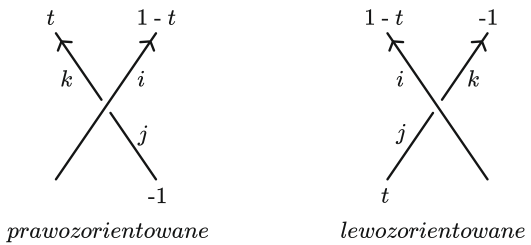
\includegraphics[scale=0.5]{3/images/1}
\end{center}

Orientację skrzyżowania wyznacza kierunek nadrzędnego łuku. Dla pierwszego skrzyżowania z Rysunku 1. łuk przechodzący nad przechodzi ze strony lewej do prawej, czyli jest prawozorientowany, 
analogicznie dla skrzyżowania lewozorientowanego.

\begin{definicja}
   Zdefinujemy macierz $A_+$ wymiaru $n \times n$, gdzie $n$ jest liczbą skrzyżowań (i łuków - zobacz dowód Lematu 3.13) według poniższej procedury. Powtórzymy
   ją dla każdego skrzyżowania $l$ w węźle:

   \begin{enumerate}
   \item Jeśli skrzyżowanie $l$ jest prawozorientowane i łuk $i$ przechodzi nad łukami $j$, $k$ (Rysunek 1.), to w wierszu $l$ wpisujemy $1 - t$ w kolumnie $i$, $-1$ w kolumnie $j$ oraz $t$ w kolumnie $k$
   \item Jeśli skrzyżowanie $l$ jest lewozorientowane i łuk $i$ przechodzi nad łukami $j$, $k$ (Rysunek 1.), to w wierszu $l$ wpisujemy $1-t$ w kolumnie $i$, $t$ w kolumnie $j$ oraz $-1$ w kolumnie $k$
   \end{enumerate}

   Wszystkie pozostałe wyrazy w wierszu $l$ są równe 0. Może się zdarzyć przypadek, kiedy jakieś $i, j, k$ są tym samym łukiem. Wtedy we właściwej kolumnie wpisujemy sumę wyrazów opisanych powyżej.
   Dla przykładu (Rysunek 2.), jeżeli $j=k$ dla jakiegoś lewozorientowanego skrzyżowania, to wpisujemy $-1+t$ w kolumnie $j$ ($=k$).

   \begin{center}
      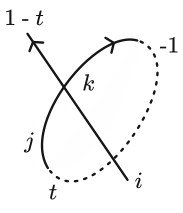
\includegraphics[scale=0.5]{3/images/2}
   \end{center}
\end{definicja}

\begin{wniosek}
   Jeżeli przyjmiemy $t = -1$ to dostaniemy macierz standardowych równanań kolorujących.
\end{wniosek}

\begin{proof}
   Dowód polega na porównaniu definicji $\Delta_L$ i $\det(L)$.
\end{proof}

\begin{przyklad}
   Pokażemy bardzo elementarnie na przykładzie trójliścia jak wyznaczyć macierz.
   Nadajemy etykiety dla skrzyżowań i łuków. Następnie rozpoznajemy orientację skrzyżowań. Narysujemy zatem rozpatrywany węzeł w taki sposób,
   by każde skrzyżowanie odpowiadało jednemu z Rysunku 1.

   \begin{center}
      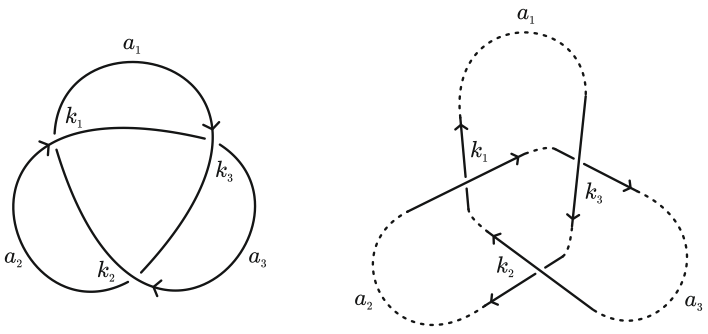
\includegraphics[scale=0.5]{3/images/3}
   \end{center}

   Przyjrzymy się teraz samym skrzyżowaniom. Wielomiany przyporządkujemy zgodnie z podaną procedurą.
   
   \begin{center}
      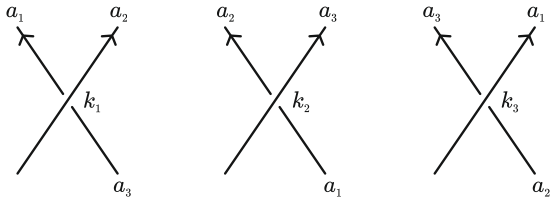
\includegraphics[scale=0.5]{3/images/4}
   \end{center}

   Wtedy odpowiadająca jemu macierz wygląda następująco:
   
   $$
   A_+ = 
   \left( \begin{array}{ccc}
   t & 1-t & -1 \\
   -1 & t & 1-t \\
   1-t & -1 & t
   \end{array} \right)
   $$ 
\end{przyklad}


%--------------------------------------


\subsection{Macierz  i wielomian Alexandera}

\begin{definicja}
   Macierz $A$ wymiaru $(n-1) \times (n-1)$ powstała poprzez usunięcie dowolnego wiersza i dowolnej kolumny z macierzy $A_+$
   nazywamy macierzą Alexandera węzła $L$. Wyznacznik macierzy Alexandera jest nazywany wielomianem Alexandera węzła $L$ i oznaczany przez $\Delta_L(t)$ ($\Delta(L)$).
   Wyznacznik macierzy $0 \times 0$ definiujemy jako $1$.
   
   $\newline$
   
   Jeżeli nie zostanie powiedziane inaczej macierz Aleksandera $A$ będzie minorem $A_+^{(1,1)}$.
\end{definicja}

\begin{przyklad}
   Wielomian Alexandera dla przykładu - trójliścia wynosi $\Delta_3(t) = t^2 - t + 1$. Aby się przekonać obliczymy wyznacznik macierzy $A_+^{(3,1)}$:

   $$
   \Delta_3(t) = \det \left( \begin{array}{ccc}
   1-t & -1 \\
   t & 1-t
   \end{array} \right) = (1-t)^2 - (-t) = 1 + t^2 -2t + t = t^2 - t + 1  
   $$ 
\end{przyklad}

\begin{wniosek}
   Wielomian Alexandera nie zależy od tego, który wiersz i którą kolumnę usuniemy.
\end{wniosek}  

\begin{proof}
   Pokażemy, że wyznacznik macierzy powstałej przez usunięcie $j$-kolumny oraz $i$-wiersza trzyma w relacji $\stackrel{\bullet}{=}$ wyznacznik minora $(1,1)$.
   
   $$
   \det A^{(1,1)} = \det( A_2^{(1)}, A_3^{(1)}, \cdots , A_n^{(1)} )
   $$

   Rozważmy wyznacznik macierzy $\det A^{(1, j)} = \det (A_1^{(1)}, A_2^{(1)}, \cdots, A_{j-1}^{(1)}, A_{j+1}^{(1)}, \cdots,  A_n^{(1)})$.
   Korzystajac z tego, że suma wierszy oraz kolumn wynosi $0$, możemy do $A_1^{(1)}$ dodać pozostałe kolumny otrzymując
   $\det A^{(1, j)} = \det (-A_j^{(1)}, A_2^{(1)}, \cdots, A_{j-1}^{(1)}, A_{j+1}^{(1)}, \cdots, A_n^{(1)})$. Odpowiednia liczba transpozycji kolumn i wyciągnięcie $-1$ z $A_j^{(1)}$ daje 
   $$
      \det A^{(1, j)} = (-1)^{j+1} \det A^{(1,1)}
   $$
   
   Podobnie postępujemy z wierszami i ostatecznie
   
   $$\det A^{(i, j)} = (-1)^{(i+1+j+1)} \det A^{(1,1)} =  (-1)^{(i+j)} \det A^{(1,1)} \stackrel{\bullet}{=} \det A^{(1,1)}$$
\end{proof}

\begin{przyklad}
   Obliczając wyznacznik macierzy $A_+^{(1,2)}$ dla trójliścia z przykładu powyżej dostaniemy $\Delta_3'(t) = -(t^2 - t + 1)$, czyli  $-\Delta_3(t)$.
\end{przyklad}

Podczas wyznaczania wielomianu Alexandera dokonaliśmy wyborów, które mają wpływ na postać wielomianu, tj:
wybór diagramu, etykietowanie łuków i skrzyżowań. Rożne wybory mogą prowadzić do różnych wielomianów Alexandera.

\begin{twierdzenie}
   Klasa równoważności relacji $\stackrel{\bullet}{=}$ wielomianów Alexandra $\Delta_L(t)$ jest dobrze zdefiniowanym
   niezmiennikiem zorientowanych węzłów, tzn relacja $\Delta_L^1(t) \stackrel{\bullet}{=} \Delta_L^2(t)$ jest zawsze utrzymana.
\end{twierdzenie}

\begin{proof}
   Twierdzenie to jest analogiczne do tego, że wyznacznik (zobacz <a href="">rodział kolorowań</a>) jest niezmiennikiem węzła.
   Ten fakt opiera się na zależności pomiędzy wyznacznikiem, a grupą kolorowań. 
   Moglibyśmy powyższe twierdzenie szybko udowodnić przytaczając zależność 
   pomiędzy wielomianem Alexandera, a obiektem zwanym modułem Alexandera, tzn modułem pierścienia $\mathbb{Z}[t, t^{-1}]$. 
   Nie chcemy się zagłębiać w teorię modułów, więc powyższe twierdzenie udowodnimy sprawdzając, że po wykonaniu ruchów Reidemeistera wielomian pozostaje w relacji $\stackrel{\bullet}{=}$.
   
   $\newline$
   
   Przy dowodzeniu za pomocą ruchów Reidemeistera patrzymy jak zmienia się wyznacznik po wykonaniu ruchu.
   
   \begin{enumerate}
      \item I ruch Reidemeistera
         
         $\newline$

         Można założyć bez straty ogólności, że ruch jest wykonywamy pomiędzy skrzyżowaniami $x$ i $y$ na $k$-łuku. Macierz $A_+$ jest wymiaru $n \times n$. Macierz $A$ uzyskamy
         usuwając pierwszy wiersz i pierwszą kolumnę.
         
         $$ 
          A_+ =  \begin{pmatrix}
         A_{1,1} & \cdots & A_{1,n-1} & k_1 \cr
         A_{2,1} & \cdots & A_{2,n-1} & k_2 \cr
          \vdots & \vdots & \cdots    & \vdots \cr
         A_{x,1} & \cdots & A_{x,n-1} & k_x \cr
         A_{y,1} & \cdots & A_{y,n-1} & k_y 
         \end{pmatrix}, \qquad A =          
         \begin{pmatrix}
         A_{2,2} & \cdots & A_{2,n-1} & k_2 \cr
          \vdots & \vdots & \cdots    & \vdots \cr
         A_{x,2} & \cdots & A_{x,n-1} & k_x \cr
         A_{y,2} & \cdots & A_{y,n-1} & k_y 
         \end{pmatrix}
         $$
         
         Wykonanie I ruchu Reidemeistera dodaje nowe skrzyżowanie (dodajemy jako ostatni wiersz), co wiąże się ze zmianą etykiet łuków.
         Pewna część kolumny $k$-łuku pozostanie bez zmian (oznaczymy ją przez $l$), pozostała część tej kolumny
         przejdzie na kolumnę łuku oznaczonego jako $m$. By nie ustalać kolejności etykietowania zauważamy zależność

         $$
         (*) \qquad \qquad \forall i \in I \quad k_i = l_i+ m_i,
         $$
         
         przy czym dokładnie jeden ze składników sumy jest równy $0$, a $I$ jest zbiorem etykiet skrzyżowań. Ruch ten powiększy wymiar macierzy do $n + 1$.
         
         $$
         A_+' =  \begin{pmatrix}
         A_{1,1} & \cdots & A_{1,n-1} & l_1 & m_1 \\
         A_{2,1} & \cdots & A_{2,n-1} & l_2 & m_2\\
         \vdots & \vdots & \cdots & \vdots \\
         A_{n-2,1} & \cdots & A_{n-2,n-1} & l_{n-2} & m_{n-2} \\
         A_{x,1} & \cdots & A_{x,n-1} & k_x & 0 \\
         A_{y,1} & \cdots & A_{y,n-1} & 0 & k_y \\
         0     & \cdots   &  0 & p(t) & -p(t)
         \end{pmatrix}
         $$
         
         gdzie $p(t), q(t) \in \{ -1,1,-t,t \}$ oraz $p(t)+q(t) = \pm (t-1)$. Następnie $m$-kolumnę dodajemy do $l$-kolumny.
         Zgodnie z $(*)$ dostajemy macierz, która po wykreśleniu pierwszej kolumny i pierwszego
         wiersza wygląda następująco:
         
         $$
         A' = \begin{pmatrix}
         A_{2,2} & \cdots & A_{2,n-1} & k_2 & m_2\\
         \vdots & \vdots & \cdots    & \vdots \\
         A_{n-2,2} & \cdots & A_{n-2,n-1} & k_{n-2} & m_{n-2} \\
         A_{x,2} & \cdots & A_{x,n-1} & k_x & 0 \\
         A_{y,2} & \cdots & A_{y,n-1} & k_y & k_y \\
         0     & \cdots   &    0      & 0 & -p(t)
         \end{pmatrix}
         $$
         
         Stosując rozwinięcie Laplace'a względem ostatniego wiersza otrzymujemy: 
         
         $$
         \det A = \Delta_L^1(t) \stackrel{\bullet}{=} \Delta_L^2(t) = \det A' = \pm p(t) \det A
         $$
   
   
      \item II ruch Reidemeistera
         
         $\newline$
         
         Ruch ten jest wykonywany na $l$-łuku, pomiędzy skrzyżowaniami $u$ i $v$ oraz $k$-łuku, pomiędzy skrzyżowaniami $x$ i $y$. Łukiem górnym jest $k$-łuk.
         Usuwamy pierwszy wiersz i pierwsza kolumnę otrzymując macierz $A$:
         
         $$
         A =  \begin{pmatrix}
         A_{2,2} & \cdots & A_{2,n-2} & k_2 & l_2 \\
         \vdots & \vdots & \cdots    & \vdots \\
         A_{n-4,2} & \cdots & A_{n-4,n-2} & k_{n-4} & l_{n-4} \\
         A_{x,2} & \cdots & A_{x,n-2} & k_x & 0 \\
         A_{y,2} & \cdots & A_{y,n-2} & k_y &0 \\
         A_{u,2} & \cdots & A_{u,n-2} & 0 & l_u \\
         A_{v,2} & \cdots & A_{v,n-2} & 0 & l_v
         \end{pmatrix}
         $$
         
         Po wykonaniu ruchu Reidemestera wymiar macierzy powiększy się o $2$. Zatem macierz Alexandera przyjmuje postać:
         
         $$
         A' = \begin{pmatrix}
         A_{2,2} & \cdots & A_{2,n-2} & k_2 & m_2 & o_2 & 0 \\
         \vdots & \vdots & \cdots    & \vdots & & & \vdots \\
         A_{n-4,2} & \cdots & A_{n-4,n-2} & k_{n-4} & m_{n-4} & o_{n-4} & 0  \\
         A_{x,2} & \cdots & A_{x,n-2} & k_x & 0 & 0 & 0 \\
         A_{y,2} & \cdots & A_{y,n-2} & k_y & 0 & 0 & 0 \\
         A_{u,2} & \cdots & A_{u,n-2} & 0 & l_u & 0 & 0 \\
         A_{v,2} & \cdots & A_{v,n-2} & 0 & 0 & l_v & 0 \\
         0 & \cdots & 0 & -p(t)-q(t) & p(t) & 0 & q(t) \\
         0 & \cdots & 0 & -p(t)-q(t) & 0 & p(t) & q(t) \\
         \end{pmatrix}
         $$
         
         
         gdzie dzięki $(*)$ zachodzi $l = m + o$. Wykonamy kolejno operacje macierzowe: od ostatniego wiersza odejmiemy wiersz przedostatni,
         do $m$-kolumny dodamy $o$-kolumnę, rozwiniemy względem ostatniego wiersza otrzymując:

         $$
         \det A' = 
         \pm p(t) \;  \det \begin{pmatrix}
         A_{2,2} & \cdots & A_{2,n-2} & k_2 & l_2 & 0 \\
          \vdots & \vdots & \cdots    & \vdots \\
         A_{n-4,2} & \cdots & A_{n-4,n-2} & k_{n-4} & l_{n-4} & 0  \\
         A_{x,2} & \cdots & A_{x,n-2} & k_x & 0 & 0 \\
         A_{y,2} & \cdots & A_{y,n-2} & k_y & 0 & 0 \\
         A_{u,2} & \cdots & A_{u,n-2} & 0 & l_u & 0 \\
         A_{v,2} & \cdots & A_{v,n-2} & 0 & l_v & 0 \\
         0 & \cdots & 0 & -p(t)-q(t) & p(t) & q(t)
         \end{pmatrix}
         $$
         
         Rozwijamy względem ostatniej kolumny i mamy:
         
         $$
         \det A = \Delta_L^1(t) \stackrel{\bullet}{=} \Delta_L^2(t) = \det A' = \pm p(t)q(t) \det A
         $$

         
         
      \item  III ruch Reidemeistera
         
         $\newline$
         
         Ruch ten nie zmienia ilości skrzyżowań i łuków, zatem na mocy faktów z algebry liniowej:
         
         \begin{enumerate}
            \item zamiana miejscami dwóch dowolnych kolumn lub wierszy macierzy zachowuje wartość bezwzględną jej wyznacznika, lecz zmienia jego znak
            \item dodając lub odejmując od dowolnego wiersza/kolumny inny wiersz/kolumnę lub kombinacje liniowe innych wierszy/kolumn nie zmieniamy wartości wyznacznika
         \end{enumerate}
         
         zachodzi $\Delta_L^2 = \pm \Delta_L^2$, zatem wielomiany są w relacji $\stackrel{\bullet}{=}$.

   \end{enumerate}
   

   Aby dowód był kompletny potrzeba sprawdzić jeszcze jeden, trudny krok. Mianowiecie, efekt zmiany orientacji. 
   To pokaże, że wielomian Alexandera odwróconego węzła $L$ jest uzyskany z wielomianu Alexandera węzła $L$
   przez zamianę $t$ na $t^{-1}$, pomnożenie przez właściwą potęgę $t$ i być może pomnożenie przez $-1$.
   Argument, który za tym stoi wymaga znajomości topologii algebraicznej, tj. powierzchni Seiferta, zatem ten fakt przyjmiemy na wiarę.
   (Alexander nie był w stanie znaleźć dowodu; pierwszy poprawny dowód podał Seifert).
\end{proof}

\begin{wniosek}
   Jeżeli dla dwóch węzłów wielomiany Alexandera są rożne, to na pewno te węzły nie są równoważne. Niestety nie możemy powiedzieć odwrotnie. Istnieją
   dwa różne węzły, dla których wielomiany będą w relacji $\stackrel{\bullet}{=}$.
\end{wniosek}

\begin{przyklad}
   Rozważmy trudniejszy przykład. Niech to będzie $(2,n)$-torus, który jest pokazany na Rysunku 5.
   Wielomian Alexandera tak opisanego diagramu dany jest przez wyznacznik minora $(n-1) \times (n-1)$ macierzy:

   $$
   \begin{pmatrix}
   1-t & -1 & 0 & 0 & \cdots & 0 \\
   t & 1-t & -1 & 0 & \cdots & 0 \\
   0 & t & 1-t & -1 & \cdots & 0 \\
    &  &  & \vdots & 1-t & -1 \\
   0 & \cdots & \cdots & 0 & t & 1-t \\
   \end{pmatrix}
   $$

   Aby wyznaczyć go dokładnie potrzeba dość szczegółowego argumentu indukcyjnego
   (wyznacznik wynosi $\frac{(t^n - 1)}{(t+1)})$.
   Bez wyliczania łatwo możemy stwierdzić, że dla różnych, dodatnich $n$ wielomiany Alexandera są również różne. 

   \begin{center}
   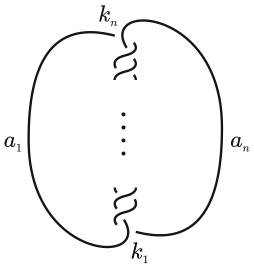
\includegraphics[scale=0.5]{3/images/5}
   \end{center}
   
   
   Zauważmy wpierw, że współczynnikiem przy wyrazie najniższego stopnia - wyrazie wolnym jest wyznacznik macierzy uzyskanej
   przez podstawienie $t =0$.
   Wtedy wynik to $1$. Współczynnik przy wyrazie najwyższego stopnia jest wyznacznikiem macierzy zawierającej
   jedynie $t$ wyrażeń w powyższej macierzy, tzn przez usunięcie wszystkich $\pm 1$. Ostatecznie wyznacznik wynosi $t^n-1$.  

   $\newline$

   Stąd wielomian Alexandera dla węzła typu $(2,n)$-torus jest stopnia dokładnie $n-1$.
   W szczególności węzły te tworzą niekończoną rodzinę rozłącznych węzłów, z czego każdy jest rozróżniany
   przez wielomian Alexandera.
\end{przyklad}

\begin{twierdzenie}
   Niech $L$ będzie zorientowany węzłem.

   \begin{enumerate}
      \item $\Delta_{mL}(t) = \Delta_{L}(t^{-1})$
      \item $\Delta_{rL}(t) = \Delta_{L}(t^{-1})$
   \end{enumerate}
\end{twierdzenie}

\begin{proof}
   Aby udowodnić $1)$ ustalmy diagram $D$ węzła $L$ i odbijmy go względem pionowej osi symetrii. Otrzymamy diagram $mD$ węzła $mL$. Weźmy
   dowolne skrzyżowanie diagramu $D$ i rozważmy odpowiadające temu skrzyżowanie w $mD$.
   
   \begin{center}
   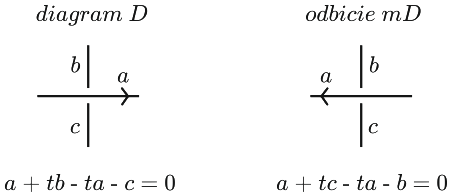
\includegraphics[scale=0.5]{3/images/6}
   \end{center}

   Współczynniki równania po lewo definiują macierz, której wyznacznik wynosi $\Delta_L(t)$ i jeżeli zastąpimy $t$ przez $t^{-1}$ dostaniemy macierz $P$, której wyznacznikiem jest $\Delta_L(t^{-1})$.
   
   Podobnie współczynniki równania po prawej stronie wyznaczają macierz $Q$, której wyznacznik to $\Delta_{mL}(t)$. Teraz zauważmy, że równanie po lewej z $t$ zastąpionym przez $t^{-1}$ jest dokładnie
   równaniem po prawej stronie pomnożonym przez $-t^{-1}$. Wtedy $P = -t^{-1} Q$ oraz
   
   $$
   \Delta_L(t^{-1}) = \det(P) = (-t)^{-m}\det(Q) = (-t^{-1})^{m}\Delta_{mL}(t) \stackrel{\bullet}{=} \Delta_{mL}(t)
   $$

   jest spełnione. 
   
   $\newline$
   
   Dowód $2)$ jest analogiczny.
\end{proof}


%--------------------------------------


\subsection{Suma spójna}

\begin{twierdzenie}
   Niech $J$ i $K$ będą zorientowanymi węzłami. Wtedy $\Delta_{J\#K}(t) \stackrel{\bullet}{=} \Delta_J(t) \Delta_K(t)$
\end{twierdzenie}

\begin{proof}
   Ustalmy diagramy dla węzłów $J$ i $K$ jak pokazano poniżej. Bez straty ogólności możemy poetykietować łuki i skrzyżowania zgodnie ze wskazanymi na Rysunku 7.

   \begin{center}
   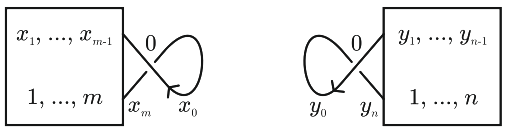
\includegraphics[scale=0.5]{3/images/7}
   \end{center}
   
   Oznaczmy przez $A$ i $B$ macierze powstałe z wielomianów rownania kolorujacego dla $J$ i $K$. Usuńmy pierwszy wiersz i pierwszą kolumnę w każdym przypadku. Wtedy
   
   $$
   \Delta_J(t) = \det(A), \qquad 
   \Delta_K(t) = \det(B)
   $$
   
   Otrzymaliśmy poniższy diagram dla $J\#K$.
     
   \begin{center}
   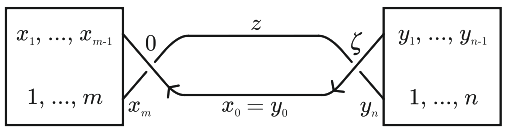
\includegraphics[scale=0.5]{3/images/8}
   \end{center}

   Mamy następujące łuki: $x_0 = y_0, x_1, \cdots, x_m, y_1, \cdots, y_m, z$, oraz skrzyżowania: $0, 1, \cdots, m$ z wezła $J$, następnie $1, \cdots, n$ z węzła $K$ oraz $\zeta$.
   Równania w węźle $J\#K$ w skrzyżowaniach $1, \cdots, m$ są dokładnie takie jak w węźle $J$, a dla skrzyżowań $1, \cdots , n$ takie jak w $K$. Dla skrzyżowania
   $\zeta$ równianie to ma postać $(1-t)y_0 + tz - y_n = 0$. 
   To pokazuje, ze jest $\Delta_{J\#K}(t)$ wyznacznikiem macierzy
   
   $$
   \begin{pmatrix}
   A & \cdots & A &  &  \\
   \vdots & \vdots & \vdots  &  \\
   A & \cdots & A &  & \\
    &  &  & B & \cdots & B  \\
    &  &  & \vdots  & \vdots & \vdots & \\
    &  &  & B & \cdots & B  \\
    &  &  &  &  & -1 & t
   \end{pmatrix}
   $$
   
   Tutaj również usuwamy pierwszy wiersz i kolumnę. Wtedy spełnione jest równanie:
   
   $$
   \Delta_{J\#K}(t) = t \Delta_{J}(t) \Delta_{K}(t) \stackrel{\bullet}{=} \Delta_{J}(t) \Delta_{K}(t)
   $$
\end{proof}


%--------------------------------------


\subsection{Równoważna defnicja}

\begin{definicja}
   Jak wspomniano wcześniej wielomiany Alexandera można wprowadzić na kilka sposobów. W tej pozycji chodziło o to, by zrobić to elementarnie. Innym sposobem 
   jest skonstruowanie funkcji $\Delta: \mathbb{L} \to \mathbb{Z}(t^{\pm 1/2})$ takiej, że dla dwóch równoważnych węzłów $L_1, L_2$ mamy równość $\Delta_{L_1} = \Delta_{L_2}$ oraz spełniającej:

   \begin{enumerate}
      \item $\Delta(   
\includegraphics[scale=0.5]{3/images/l2}    ) = 1$
      \item  $\Delta(L_+) - \Delta(L_-) + (t^{1/2} - t^{-1/2})\Delta(L_0) = 0$, gdzie
         
         \begin{center}
         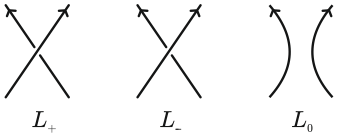
\includegraphics[scale=0.5]{3/images/9}
         \end{center}

   \end{enumerate}

   gdzie $\mathbb{L}$ oznacza zbiór wszystkich węzłów. Zobaczymy kilka przykładów:
\end{definicja}

\begin{przyklad}
   Znajdziemy wielomian Alexandera rozłącznej sumy dwóch niewęzłów, tak jak $\Delta( 
\includegraphics[scale=0.5]{3/images/l1} )$.
   Oznaczymy ten węzeł jako $L_0$ i skorzystamy z własności $2)$.

   $$
   0 = \Delta(L_+) - \Delta(L_-) + (t^{1/2} - t^{-1/2}) \Delta(L_0)
   $$ $$
   0 = \Delta (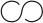
\includegraphics[scale=0.5]{3/images/l3}) - \Delta (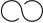
\includegraphics[scale=0.5]{3/images/l4}) + (t^{1/2} - t^{-1/2}) \Delta(L_0)
   $$ $$
   0 = \Delta (
\includegraphics[scale=0.5]{3/images/l2}) - \Delta (
\includegraphics[scale=0.5]{3/images/l2}) + (t^{1/2} - t^{-1/2}) \Delta(L_0)
   $$ $$
   0 = (t^{1/2} - t^{-1/2}) \Delta(L_0)
   $$

   i stąd otrzymujemy, że $\Delta(L_0) = 0$.
\end{przyklad}

\begin{przyklad}
   Znajdziemy wielomian Alexandera węzła Hopfa, czyli $\Delta( 
\includegraphics[scale=0.5]{3/images/l5} )$. 
   Oznaczymy ten węzeł jako $L_+$ i
   skorzystamy z własności $2)$ na górnym skrzyżowaniu oraz z pierwszego przykładu.

   $$
   0 = \Delta(L_+) - \Delta(L_-) + (t^{1/2} - t^{-1/2}) \Delta(L_0)
   $$ $$
   0 = \Delta(L_+) - \Delta( 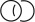
\includegraphics[scale=0.5]{3/images/l6} ) + (t^{1/2} - t^{-1/2}) \Delta( 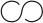
\includegraphics[scale=0.5]{3/images/l3} )
   $$ $$
   0 = \Delta(L_+) - \Delta(L_-) + (t^{1/2} - t^{-1/2}) \Delta( 
\includegraphics[scale=0.5]{3/images/l2} )
   $$ $$
   0 = (t^{1/2} - t^{-1/2}) \Delta(L_0)
   $$

   i stąd otrzymujemy, że $\Delta( 
\includegraphics[scale=0.5]{3/images/l5} ) = t^{1/2} - t^{-1/2}$.
\end{przyklad}






% Remigiusz
\section{Wielomian Jonesa}

Przed wprowadzeniem kolejnego wielomianowego niezmiennika przyjrzymy się ich historii.
Znamy już wielomian J. Alexandera, który został odkryty około roku 1928.
W 1969 J. Conway znalazł sposób na wyznaczenie wielomianu Alexandera dla dowolnego splotu przy użyciu tak zwanej relacji kłębiastej\footnote{skein relation}.
Jest to równanie wiążące wielomian splotu z wielomianami splotów o zmienionym jednym skrzyżowaniu w diagramie splotu wyjściowego.
Relacja kłębiasta okazała się kluczem do sukcesu.

Vaughan Jones, matematyk nowozelandzki, odkrył w 1984 nowy wielomian dla splotów jako produkt uboczny podczas pracy nad algebrami operatorowymi.
Odkrycie Jonesa było przełomowe, a już cztery miesiące później ogłoszono znalezienie nowego niezmiennika: wielomianu HOMFLY, którego nazwa pochodzi od pierwszych liter nazwisk odkrywców, to jest: Hoste, Ocneanu, Millett, Freyd, Lickorish, Yetter.

Aby lepiej zrozumieć wielomian Jonesa przyjrzymy się najpierw prostszej konstrukcji, nawiasowi Kauffmana.
Później zajmiemy się węzłami alternującymi.
% W tej sekcji zbadamy inny wielomianowy niezmiennik węzłów, wielomian Jonesa.
% Został odkryty w 1984 roku przez Vaughana Jonesa, znajduje zastosowanie między innymi przy badaniu węzłów przemiennych.

\subsection{Nawias Kauffmana}
Zaczniemy od zdefiniowania nawiasu Kauffmana.
Przypomnijmy, wielomian Laurenta zmiennej $X$ to formalny symbol $f=a_r X^r + \ldots + a_s X^s$, gdzie $r, s, a_r, \ldots, a_s$ są całkowite i $r \le s$.

Poszukujemy niezmiennika dla splotów o kilku prostych własnościach.
Przede wszystkim żądamy, by niewęzłowi przypisany był wielomian $1$: $\langle \NieWezel \rangle = 1$.
Po drugie chcemy móc wyznaczać nawiasy znając je dla prostszych splotów, co zapiszemy symbolicznie $\langle \PrawyKrzyz \rangle = A \langle \PrawyGladki \rangle + B \langle \LewyGladki \rangle$.
Zależy nam wreszcie na tym, by móc dodać do splotu trywialną składową: $\langle L \cup \NieWezel \rangle = C \langle L \rangle$.

Prosty rachunek pokazuje wpływ drugiego ruchu Reidemeistera na nawias:
\[
	\langle \begin{tikzpicture} [scale=0.025,baseline=-3]
			\path[TEXTARC] (0,10) .. controls (10,5) and (10,-9) .. (0,-14);
			\path[TEXTARC] (10,10) .. controls (8,9) .. (7,8);
			\path[TEXTARC] (3,4.5) .. controls (-1,0) and (-1,-4) .. (3,-8);
			\path[TEXTARC] (10,-14) .. controls (8,-13) .. (7,-12);
	\end{tikzpicture} \rangle = (A^2 + ABC + B^2) \langle \LewyGladki \rangle + BA \langle \PrawyGladki \rangle\stackrel{?}{=} \langle \PrawyGladki \rangle.
\]

Aby zachodziła ostatnia równość wystarczy (chociaż wcale nie trzeba) przyjąć $B = A^{-1}$, co wymusza na nas $C = -A^2 - A^{-2}$.
W ten sposób odkryliśmy następującą definicję.

\begin{definicja}
	\emph{Nawias Kauffmana} $\langle D \rangle$ dla diagramu splotu $D$ to wielomian Laurenta zmiennej $A$, który jest niezmienniczy ze względu na gładkie deformacje diagramu, a przy tym spełnia trzy aksjomaty:
	\begin{enumerate}
		\item $\langle \NieWezel \rangle=1$
		\item $\langle D \sqcup \NieWezel \rangle = (-A^{-2} - A^2) \langle D \rangle$
		\item $\langle \PrawyKrzyz \rangle = A \langle \PrawyGladki \rangle + A^{-1} \langle \LewyGladki  \rangle$
	\end{enumerate}
\end{definicja}

Tutaj $\NieWezel$ oznacza standardowy diagram dla niewęzła, $D \sqcup \NieWezel$ jest diagramem, który powstaje z $D$ przez dodanie nieprzecinającej go krzywej zamkniętej, zaś trzy symbole $\PrawyKrzyz$, $\PrawyGladki$ oraz $\LewyGladki $ odnoszą się do diagramów, które są identyczne wszędzie poza małym obszarem.
Diagramy $\PrawyGladki$ oraz $\LewyGladki$ nazywa się odpowiednio dodatnim (prawym) i ujemnym (lewym) wygładzeniem $\PrawyKrzyz$

\begin{lemat}
	Nawias Kauffmana dowolnego diagramu można wyznaczyć w skończonie wielu krokach.
\end{lemat}

\begin{proof}
	Jeżeli diagram $D$ ma $n$ skrzyżowań, to nieustanne stosowanie aksjomatu trzeciego pozwala na zapisanie $\langle D \rangle$ jako sumy $2^n$ składników, z których każdy jest po prostu zamkniętą krzywą i ma trywialny nawias ($\langle \MalyNieWezel \rangle = 1$).
	Nawias sumy wyznacza się korzystając z drugiego aksjomatu.
\end{proof}

Przedstawimy teraz wpływ ruchów Reidemeistera na nawias Kauffmana.

\begin{lemat}
	Pierwszy ruch Reidemeistera zmienia nawias Kauffmana zgodnie z poniższą regułą.
	Pozosałe ruchy Reidemeistera nie zmieniają nawiasu.
	\[
		% pierwszy ruch Reidemeistera
		\left\langle\begin{tikzpicture}[scale=0.05, baseline=-6]
			\clip (-12,-12) rectangle (1,7);
			\path[ARC] (-10,7) .. controls (-10,3) and (-10,0) .. (-6,-4);
			\path[ARC] (-6,0) .. controls (2,8) and (2,-10) .. (-6,-4);
			\path[ARC] (-10,-11) .. controls (-10,-8) and (-10,-5) .. (-9,-4);
		\end{tikzpicture}\right\rangle
		= -A^{-3}
		\left\langle\ \begin{tikzpicture}[scale=0.05,baseline=-6]
			\path[ARC] (-10,7) -- (-10,-11);
		\end{tikzpicture}\ \right\rangle
		\,\bullet\,
		% drugi ruch Reidemeistera
		\left\langle\begin{tikzpicture} [scale=0.04,baseline=-5]
			\path[ARC](0,10) .. controls (10,5) and (10,-9) .. (0,-14);
			\path[ARC] (10,10) .. controls (8,9) .. (7,8);
			\path[ARC] (3,4.5) .. controls (-1,0) and (-1,-4) .. (3,-8);
			\path[ARC] (10,-14) .. controls (8,-13) .. (7,-12);
		\end{tikzpicture}\right\rangle
		=
		\left\langle\ \begin{tikzpicture} [scale=0.04, baseline=-5]
		\path[ARC] (0,10) .. controls (3,8) and (3,0) .. (3,-2) .. controls (3,-4) and (3,-12) .. (0,-14);
		\path[ARC] (10,10) .. controls (7,8) and (7,0) .. (7,-2) .. controls (7,-4) and (7,-12) .. (10,-14);
		\end{tikzpicture}\ \right\rangle
		\,\bullet\,
		% trzeci ruch Reidemeistera
		\left\langle\begin{tikzpicture} [scale=0.04, auto, baseline=-6]
			\path[ARC] (-10,10) -- (-6.6,6);
			\path[ARC] (-4,3) -- (10,-14);
			\path[ARC] (10,10) -- (6.6,6);
			\path[ARC] (4,3) -- (1.6,0);
			\path[ARC] (-1.6,-4) -- (-10,-14);
			\path[ARC] (-14,-2) .. controls (-6, -2) and (-6,8) .. (0,8);
			\path[ARC] (14,-2) .. controls (6, -2) and (6,8) .. (0,8);
		\end{tikzpicture}\right\rangle
		=
		\left\langle\begin{tikzpicture} [scale=0.04, auto, baseline=-6]
			\begin{scope}[xshift=1300,rotate=180,yshift=110]
				\path[ARC] (-10,10) -- (-6.6,6);
				\path[ARC] (-4,3) -- (10,-14);
				\path[ARC] (10,10) -- (6.6,6);
				\path[ARC] (4,3) -- (1.6,0);
				\path[ARC] (-1.6,-4) -- (-10,-14);
				\path[ARC] (-14,-2) .. controls (-6, -2) and (-6,8) .. (0,8);
				\path[ARC] (14,-2) .. controls (6, -2) and (6,8) .. (0,8);
			\end{scope}
		\end{tikzpicture}\right\rangle.
	\]
\end{lemat}

\begin{proof}
Pierwszy ruch Reidemeistera:
\[
\left\langle\begin{tikzpicture}[scale=0.05, baseline=-6]
	\clip (-12,-12) rectangle (1,7);
	\path[ARC] (-10,7) .. controls (-10,3) and (-10,0) .. (-6,-4);
	\path[ARC] (-6,0) .. controls (2,8) and (2,-10) .. (-6,-4);
	\path[ARC] (-10,-11) .. controls (-10,-8) and (-10,-5) .. (-9,-4);
\end{tikzpicture}\right\rangle
\stackrel{K3}{=}
A\left\langle\begin{tikzpicture}[scale=0.05, baseline=-6]
	\clip (-12,-12) rectangle (1,7);
	\path[ARC] (-10,7) .. controls (-10,3) and (-9,-3) .. (-6,0);
	\path[ARC] (-6,0) .. controls (2,8) and (2,-10) .. (-6,-4);
	\path[ARC] (-10,-11) .. controls (-10,-8) and (-10,-1) .. (-6,-4);
\end{tikzpicture}\right\rangle
+A^{-1}\left\langle
\begin{tikzpicture}[scale=0.05, baseline=-6] 
	\clip (-12,-12) rectangle (1,7);
	\path[ARC] (-10,7) .. controls (-10,3) and (-7,-2) .. (-9,-4);
	\path[ARC] (-5,1) .. controls (2,8) and (2,-10) .. (-5,-5);
	\path[ARC] (-5,1) .. controls (-6.5,-0.5) and (-6.5,-3.5) .. (-5,-5);
	\path[ARC] (-10,-11) .. controls (-10,-8) and (-10,-5) .. (-9,-4);
\end{tikzpicture}\right\rangle
\stackrel{K2}{=}
A\left\langle\ 
\begin{tikzpicture}[scale=0.05, baseline=-6]
	\path[ARC] (-10,7) -- (-10,-11);
\end{tikzpicture}\ 
\right\rangle
+A^{-1}(-A^{-2}-A^2)\left\langle\ 
\begin{tikzpicture}[scale=0.05, baseline=-6] 
	\path[ARC] (-10,7) -- (-10,-11);
\end{tikzpicture}
\ \right\rangle
=
-A^{-3}\left\langle\ 
\begin{tikzpicture}[scale=0.05, baseline=-6] 
	\path[ARC] (-10,7) -- (-10,-11);
\end{tikzpicture}\ 
\right\rangle
\]
Pierwsza równość wynika z $K3$, druga z $K2$, trzecia jest oczywista.
Dla drugiego ruchu:
\begin{align*}
\left\langle\begin{tikzpicture} [scale=0.04,baseline=-5] 
	\path[ARC](0,10) .. controls (10,5) and (10,-9) .. (0,-14);
	\path[ARC] (10,10) .. controls (8,9) .. (7,8);
	\path[ARC] (3,4.5) .. controls (-1,0) and (-1,-4) .. (3,-8);
	\path[ARC] (10,-14) .. controls (8,-13) .. (7,-12);
\end{tikzpicture}\right\rangle
&\stackrel{K3}{=}
\phantom{-}A^{\phantom{-2}}
\left\langle\begin{tikzpicture} [scale=0.04,baseline=-5] 
	\clip (-2,-14) rectangle (12,10);
	\path[ARC] (0,10) .. controls (4.5,6) and (5.5,6) .. (10,10);
	\path[ARC] (0,-14) .. controls (4,-11) .. (6,-8) .. controls (12,0) and (-5,0) .. (3,-8);
	\path[ARC] (10,-14) .. controls (8.5,-13) .. (7,-12);
\end{tikzpicture}\right\rangle
+
\phantom{A}A^{-1}
\left\langle\begin{tikzpicture} [scale=0.04,baseline=-5]
	\clip (-2,-14) rectangle (12,10);
	\path[ARC] (10,10) .. controls (8,9) .. (7,8);
	\path[ARC] (10,-14) .. controls (8,-13) .. (7,-12);
	\path[ARC](10,10) .. controls (0,5) and (15,-4) .. (0,-14);	
	\path[ARC] (0,10) .. controls (10,5) and (-3,0) .. (3,-8);
\end{tikzpicture}\right\rangle
\stackrel{K1}{=}
-A^{-2}
\left\langle\begin{tikzpicture} [scale=0.04, baseline=-5]
	\clip (-2,-14) rectangle (12,10);
	\path[ARC] (0,10) .. controls (4.5,6) and (5.5,6) .. (10,10);
	\path[ARC] (0,-14) .. controls (4.5,-10) and (5.5,-10) .. (10,-14);
\end{tikzpicture}\right\rangle
+
\phantom{A}
A^{-1}
\left\langle\begin{tikzpicture} [scale=0.04,baseline=-5] 
	\clip (-2,-14) rectangle (12,10);
	\path[ARC] (10,10) .. controls (8,9) .. (7,8);
	\path[ARC] (10,-14) .. controls (8,-13) .. (7,-12);
	\path[ARC](10,10) .. controls (0,5) and (15,-4) .. (0,-14);	
	\path[ARC] (0,10) .. controls (10,5) and (-3,0) .. (3,-8);
\end{tikzpicture}\right\rangle
\\
&\stackrel{K3}{=}
-A^{-2}
\left\langle\begin{tikzpicture} [scale=0.04, baseline=-5]
	\clip (-2,-14) rectangle (12,10);
	\path[ARC] (0,10) .. controls (4.5,6) and (5.5,6) .. (10,10);
	\path[ARC] (0,-14) .. controls (4.5,-10) and (5.5,-10) .. (10,-14);
\end{tikzpicture}\right\rangle
+A^{-1}A
\left\langle\begin{tikzpicture} [scale=0.04, baseline=-5] 
	\clip (-2,-14) rectangle (12,10);
	\path[ARC] (0,10) .. controls (3,8) and (3,0) .. (3,-2) .. controls (3,-4) and (3,-12) .. (0,-14);
	\path[ARC] (10,10) .. controls (7,8) and (7,0) .. (7,-2) .. controls (7,-4) and (7,-12) .. (10,-14);
\end{tikzpicture}\right\rangle
+
A^{-1}A^{-1}
\left\langle\begin{tikzpicture} [scale=0.04, baseline=-5]
	\clip (-2,-14) rectangle (12,10);
	\path[ARC] (0,10) .. controls (4.5,6) and (5.5,6) .. (10,10);
	\path[ARC] (0,-14) .. controls (4.5,-10) and (5.5,-10) .. (10,-14);
\end{tikzpicture}\right\rangle
=%\phantom{-A^{-2}}
\left\langle\begin{tikzpicture} [scale=0.04, baseline=-5]
	\clip (-2,-14) rectangle (12,10);
	\path[ARC] (0,10) .. controls (3,8) and (3,0) .. (3,-2) .. controls (3,-4) and (3,-12) .. (0,-14);
	\path[ARC] (10,10) .. controls (7,8) and (7,0) .. (7,-2) .. controls (7,-4) and (7,-12) .. (10,-14);
\end{tikzpicture}\right\rangle
\end{align*}
Dla trzeciego ruchu:
\begin{align*}
\left\langle\begin{tikzpicture} [scale=0.04, auto, baseline=-6] 
	\path[ARC] (-10,10) -- (-6.6,6);
	\path[ARC] (-4,3) -- (10,-14);
	\path[ARC] (10,10) -- (6.6,6);
	\path[ARC] (4,3) -- (1.6,0);
	\path[ARC] (-1.6,-4) -- (-10,-14);
	\path[ARC] (-14,-2) .. controls (-6, -2) and (-6,8) .. (0,8);
	\path[ARC] (14,-2) .. controls (6, -2) and (6,8) .. (0,8);
\end{tikzpicture}\right\rangle
&\stackrel{K3}{=}
A
\left\langle\begin{tikzpicture} [scale=0.04, auto, baseline=-6] 
	\path[ARC] (-10,10) -- (-6.6,6);
	\path[ARC] (10,10) -- (6.6,6);
	\path[ARC] (-14,-2) .. controls (-6, -2) and (-6,8) .. (0,8);
	\path[ARC] (14,-2) .. controls (6, -2) and (6,8) .. (0,8);
	\path[ARC] (-10,-14) .. controls (0,-3) and (0,-3) .. (10,-14);
	\path[ARC] (-4,3) .. controls (0,-2) .. (4,3);
\end{tikzpicture}\right\rangle
+A^{-1}
\left\langle\begin{tikzpicture} [scale=0.04, auto, baseline=-6]
	\path[ARC] (-14,-2) -- (14,-2);
	\path[ARC] (-10,10) .. controls (-7,6) and (-4,4) .. (-4,0);
	\path[ARC] (-10,-14) .. controls (-7,-10) and (-4,-8) .. (-4,-4);
	\path[ARC] (10,10) .. controls (7,6) and (4,4) .. (4,0);
	\path[ARC] (10,-14) .. controls (7,-10) and (4,-8) .. (4,-4);
\end{tikzpicture}\right\rangle
\stackrel{R2}{=}
A
\left\langle\begin{tikzpicture} [scale=0.04, auto, baseline=-6]
	\path[ARC] (-14,-2) -- (14,-2);
	\path[ARC] (-10,-14) .. controls (0,-3) and (0,-3) .. (10,-14);
	\path[ARC] (-10,10) .. controls (0,-1) and (0,-1) .. (10,10);
\end{tikzpicture}\right\rangle
+A^{-1}
\left\langle\begin{tikzpicture} [scale=0.04, auto, baseline=-6] 
	\path[ARC] (-14,-2) -- (14,-2);
	\path[ARC] (-10,10) .. controls (-7,6) and (-4,4) .. (-4,0);
	\path[ARC] (-10,-14) .. controls (-7,-10) and (-4,-8) .. (-4,-4);
	\path[ARC] (10,10) .. controls (7,6) and (4,4) .. (4,0);
	\path[ARC] (10,-14) .. controls (7,-10) and (4,-8) .. (4,-4);
\end{tikzpicture}\right\rangle
\\
&\stackrel{R2}{=}
A
\left\langle\begin{tikzpicture} [scale=0.04, auto, baseline=-6,yscale=-1] 
	\path[ARC] (-10,10) -- (-6.6,6);
	\path[ARC] (10,10) -- (6.6,6);
	\path[ARC] (-14,-2) .. controls (-6, -2) and (-6,8) .. (0,8);
	\path[ARC] (14,-2) .. controls (6, -2) and (6,8) .. (0,8);
	\path[ARC] (-10,-14) .. controls (0,-3) and (0,-3) .. (10,-14);
	\path[ARC] (-4,3) .. controls (0,-2) .. (4,3);
\end{tikzpicture}\right\rangle
+A^{-1}
\left\langle\begin{tikzpicture} [scale=0.04, auto, baseline=-6] 
	\path[ARC] (-14,-2) -- (14,-2);
	\path[ARC] (-10,10) .. controls (-7,6) and (-4,4) .. (-4,0);
	\path[ARC] (-10,-14) .. controls (-7,-10) and (-4,-8) .. (-4,-4);
	\path[ARC] (10,10) .. controls (7,6) and (4,4) .. (4,0);
	\path[ARC] (10,-14) .. controls (7,-10) and (4,-8) .. (4,-4);
\end{tikzpicture}\right\rangle
\stackrel{K3}{=}
\left\langle\begin{tikzpicture} [scale=0.04, auto, baseline=-6] 
\begin{scope}[xshift=1300,rotate=180,yshift=110]
	\path[ARC] (-10,10) -- (-6.6,6);
	\path[ARC] (-4,3) -- (10,-14);
	\path[ARC] (10,10) -- (6.6,6);
	\path[ARC] (4,3) -- (1.6,0);
	\path[ARC] (-1.6,-4) -- (-10,-14);
	\path[ARC] (-14,-2) .. controls (-6, -2) and (-6,8) .. (0,8);
	\path[ARC] (14,-2) .. controls (6, -2) and (6,8) .. (0,8);
\end{scope}
\end{tikzpicture}\right\rangle
\end{align*}
korzystaliśmy tu z własności drugiego ruchu.
\end{proof}

Okazało się, że użycie najprostszego, I ruchu Reidemeistera, ,,psuje'' nawias!
W akcie desperacji moglibyśmy zmienić definicję, zaniechamy tego i przejdziemy do kolejnego składnika w przepisie na wielomian Jonesa.
\subsection{Spin}
Przypomnijmy, że znak skrzyżowania na diagramie to liczba $1$ lub $-1$:
$\operatorname{sign}
	\begin{tikzpicture}[scale=0.03, baseline=-3]
	\path[TEXTARC,->] (-5,-5) -- (5,5);
	\path[TEXTARC] (5,-5) -- (1.5,-1.5);
	\path[TEXTARC,<-] (-5,5) -- (-1.5,1.5);
	\end{tikzpicture}
 = +1$,
$\operatorname{sign} \begin{tikzpicture}[scale=0.03, baseline=-3]
\path[TEXTARC,->] (5,-5) -- (-5,5);
\path[TEXTARC] (-5,-5) -- (-1.5,-1.5);
\path[TEXTARC,<-] (5,5) -- (1.5,1.5);
\end{tikzpicture} = -1$.

\begin{definicja}
	Niech $D$ będzie diagramem zorientowanego splotu lub węzła.
	\textbf{Spinem} $D$ jest $w(D) = \sum_c \operatorname{sign} c$, gdzie sumowanie przebiega po wszystkich skrzyżowaniach.
\end{definicja}

\begin{przyklad}
Spinem trójlistnika w takiej wersji jest $+3$:
\[
	\begin{tikzpicture}[scale=0.035]
		\clip (-16,-16) rectangle (16,17); %nie etykietuj
		\foreach \x in {270,30, 150}
		\path[TEXTARC,->-] (15+\x:6) .. controls (130+\x:25) and (200+\x:25) .. (225+\x:10);
		\node[red] (C1) at (30:14) {\small $+1$};
		\node[red] (C2) at (150:14) {\small $+1$};
		\node[red] (C3) at (270:14) {\small $+1$};
	\end{tikzpicture}
\]
\end{przyklad}

\begin{lemat}
Tylko I ruch Reidemeistera zmienia spin:
$
w(\begin{tikzpicture}[scale=0.025, baseline=-3]
	\clip (-12,-12) rectangle (1,7);
	\path[TEXTARC] (-10,7) .. controls (-10,3) and (-10,0) .. (-6,-4);
	\path[TEXTARC] (-6,0) .. controls (2,8) and (2,-10) .. (-6,-4);
	\path[TEXTARC] (-10,-11) .. controls (-10,-8) and (-10,-5) .. (-9,-4);
\end{tikzpicture})
=
w(\ \begin{tikzpicture}[scale=0.025,baseline=-4]
	\path[TEXTARC] (-10,7) -- (-10,-11);
\end{tikzpicture}\ )-1
$, pozostałe nie mają wpływu.
Spin nie zależy od orientacji.
\end{lemat}

\begin{proof}
Proste ćwiczenie.
\end{proof}
\subsection{Wielomian Jonesa}

\begin{definicja}
\emph{Wielomian Jonesa} zorientowanego splotu to wielomian Laurenta $V(L)\in\Z[t^{1/2},t^{-1/2}]$ określony przez
\[V(L)=\left[ (-A)^{-3w(D)}\langle D\rangle\right]_{t^{1/2}=A^{-2}},\]
gdzie $D$ to dowolny diagram dla $L$.
\end{definicja}

\begin{twierdzenie}
Wielomian Jonesa jest niezmiennikiem zorientowanych splotów.
\end{twierdzenie}

\begin{proof}
%Skorzystamy z tego, że indeks zaczepienia jest niezmiennikiem.
Wystarczy pokazać niezmienniczość $(-A)^{-3w(D)}\langle D\rangle$ na ruchy Reidemeistera.
Ale
\[
(-A)^{-3
w\left(\begin{tikzpicture}[scale=0.025, baseline=-3]
	\clip (-12,-12) rectangle (1,7);
	\path[TEXTARC] (-10,7) .. controls (-10,3) and (-10,0) .. (-6,-4);
	\path[TEXTARC] (-6,0) .. controls (2,8) and (2,-10) .. (-6,-4);
	\path[TEXTARC] (-10,-11) .. controls (-10,-8) and (-10,-5) .. (-9,-4);
\end{tikzpicture}\right)}
\left\langle\begin{tikzpicture}[scale=0.025, baseline=-3]
	\clip (-12,-12) rectangle (1,7);
	\path[TEXTARC] (-10,7) .. controls (-10,3) and (-10,0) .. (-6,-4);
	\path[TEXTARC] (-6,0) .. controls (2,8) and (2,-10) .. (-6,-4);
	\path[TEXTARC] (-10,-11) .. controls (-10,-8) and (-10,-5) .. (-9,-4);
\end{tikzpicture}\right\rangle
=
(-A)^{-3
w\left(\ \begin{tikzpicture}[scale=0.025,baseline=-4]
	\path[TEXTARC] (-10,7) -- (-10,-11);
\end{tikzpicture}\ \right)+3}
(-A)^{-3}
\left\langle\ \begin{tikzpicture}[scale=0.025,baseline=-4]
	\path[TEXTARC] (-10,7) -- (-10,-11);
\end{tikzpicture}\ \right\rangle =
(-A)^{-3
w\left(\ \begin{tikzpicture}[scale=0.025,baseline=-4]
	\path[TEXTARC] (-10,7) -- (-10,-11);
\end{tikzpicture}\ \right)}
\left\langle\ \begin{tikzpicture}[scale=0.025,baseline=-4]
	\path[TEXTARC] (-10,7) -- (-10,-11);
\end{tikzpicture}\ \right\rangle.\qedhere
\]
\end{proof}

Wielomian Jonesa jest naprawdę potężnym narzędziem.
Pozwala bowiem odróżnić dowolne dwa węzły pierwsze o co najwyżej dziewięciu skrzyżowaniach.

\begin{hipoteza}
Nie istnieje nietrywialny węzeł, którego wielomian Jonesa nie odróżnia od niewęzła.
\end{hipoteza}

\begin{twierdzenie}
Wielomianem węzła $(m, n)$-torusowego jest
\[
	\frac {t^{(m-1)(n-1):2}}{1-t^2} \cdot (1 - t^{m+1} - t^{n+1} + t^{m+n}).
\]
\end{twierdzenie}
\subsection{Relacja kłębiasta}
Dotychczas wyznaczyliśmy wielomian Jonesa jedynie dla trywialnych splotów.
Spowodowane jest to tym, że chociaż nawias Kauffmana jest przydatny przy dowodzeniu różnych własności, to zupełnie nie nadaje się do obliczeń.
Dużo lepszym narzędziem jest następujące twierdzenie.

\begin{twierdzenie}[relacja kłębiasta]
	Wielomian Jonesa spełnia równość $V(\NieWezel) = 1$ oraz relację
	\[
		t^{-1} V(L_+) - tV(L_-) + (t^{-1/2} - t^{1/2}) V(L_0) = 0,
	\]

	gdzie $L_+$, $L_-$, $L_0$ to zorientowane sploty, kóre różnią się jedynie na małym obszarze:
	$
		\begin{tikzpicture}[scale=0.03, baseline=-3]
		\path[TEXTARC,->] (-5,-5) -- (5,5);
		\path[TEXTARC] (5,-5) -- (1.5,-1.5);
		\path[TEXTARC,<-] (-5,5) -- (-1.5,1.5);
		\end{tikzpicture}
	$, 
	$
		\begin{tikzpicture}[scale=0.03, baseline=-3]
		\path[TEXTARC,->] (5,-5) -- (-5,5);
		\path[TEXTARC] (-5,-5) -- (-1.5,-1.5);
		\path[TEXTARC,<-] (5,5) -- (1.5,1.5);
		\end{tikzpicture}
	$, 
	$
		\begin{tikzpicture}[scale=0.03, baseline=-3]
		\path[TEXTARC,->] (-5,-5) .. controls (-1.5,-1.5) and (-1.5,1.5) .. (-5,5);
		\path[TEXTARC,->] (5,-5) .. controls (1.5,-1.5) and (1.5,1.5) .. (5,5);
		\end{tikzpicture}
	$.
\end{twierdzenie}

\begin{proof}
Wyraźmy wielomian Jonesa przez nawias Kauffmana i spin.
Chcemy pokazać, że
\[
A^{4}(-A)^{-3w(L_+)}\langle\PrawyKrzyz\rangle
-A^{-4}(-A)^{-3w(L_-)}\langle\LewyKrzyz\rangle
+(A^2-A^{-2})(-A)^{-3w(L_0)}\langle\PrawyGladki\rangle
=0.
\]
Ale $w(L_\pm)=w(L_0)\pm 1$, zatem to jest równoważne z $-A\langle\PrawyKrzyz\rangle +A^{-1}\langle\LewyKrzyz\rangle +(A^2-A^{-2})\langle\PrawyGladki\rangle =0$.
Z definicji nawiasu Kauffmana wnioskujemy, że
$\langle\PrawyKrzyz\rangle = A\langle\PrawyGladki\rangle+A^{-1}\langle\LewyGladki\rangle$ i $\langle\LewyKrzyz\rangle = A\langle\LewyGladki\rangle+A^{-1}\langle\PrawyGladki\rangle$.
Pierwsze równanie przemnóżmy przez $A$, drugie przez $A^{-1}$, a następnie dodajmy je do siebie.
Wtedy otrzymamy $A\langle\PrawyKrzyz\rangle-A^{-1}\langle\LewyKrzyz\rangle = A^2\langle\PrawyGladki\rangle - A^{-2}\langle\PrawyGladki\rangle$.
\end{proof}

\begin{przyklad}
	$V(
		\begin{tikzpicture}
		[scale=0.02, baseline=-3]
		\clip (-15,-9) rectangle (15,9);
		\path[TEXTARC,-<-] (1.5,-2.75) arc (-20:300:8);
		\path[TEXTARC,-<-] (-1.5,2.75) arc (160:480:8);
		\end{tikzpicture}) = -t^{5/2} - t ^{1/2}
	$ (splot Hopfa),
	$
	V(\begin{tikzpicture}[scale=0.02,baseline=-2]
	\clip (-19,-13) rectangle (19,17);
	\foreach \x in {270,30, 150}
		\path[TEXTARC,-<-] (15+\x:6) .. controls (130+\x:25) and (200+\x:25) .. (225+\x:10);
\end{tikzpicture}) = -t^4+t^3 + t
$ (trójlistnik).
\end{przyklad}
\subsection{Odwrotności, lustra i sumy}

\begin{twierdzenie}
Niech $L$ będzie zorientowanym splotem.
$V(rL)=V(L)$, $V(mL)(t)=V(L)(t^{-1})$.
\end{twierdzenie}

\begin{wniosek}
Wielomian Jonesa nie zależy od orientacji węzła (ale nie splotu!).
\end{wniosek}

\begin{proof}
Każdy węzeł ma tylko dwie orientacje, splot może mieć ich $2^n$, gdzie $n$ to liczba składowych.
\end{proof}

\begin{wniosek}
Trójlistnik nie jest równoważny ze swoim lustrem.
\end{wniosek}

\begin{proof}
W zależności od orientacji wielomianem trójlistnika jest $...$ lub $...$.
\end{proof}

\begin{twierdzenie}
Niech $L, M$ będą zorientowanymi splotami, zaś $J, K$: zorientowanymi węzłami.
\begin{enumerate}
\item $V(L \sqcup M) = (-t^{1/2} - t^{-1/2}) V(L) V(M)$,
\item $V(J \# K) = V(J) V(K)$.
\end{enumerate}
\end{twierdzenie}

\begin{proof}
Wybierzmy diagramy $D, E$ dla (odpowiednio) $L, M$.
Po podstawieniu $t^{1/2}=A^{-2}$ widzimy, że chcemy pokazać $(-A)^{-3w(D\sqcup E)}\langle D\sqcup E\rangle =(-A^2-A^{-2})(-A)^{-3(w(D)+w(E))}\langle D\rangle  \langle E\rangle$.

Oczywiście $w(D\sqcup E)=w(D)+w(E)$, więc wystarczy udowodnić, że 
\[
	\langle D\sqcup E\rangle = (-A^2-A^{-2})\langle D\rangle\langle E\rangle.
\]

Oznaczmy przez $f_1(D)$, $f_2(D)$ lewą i prawą stronę ostatniego równania.
Są to wielomiany Laurenta, które zależą tylko od $D$.
Aksjomaty Kauffmana pozwalają na pokazanie, że obie funkcje mają następujące własności:
$f_i(\NieWezel)=(-A^2-A^{-2})\langle E\rangle$, $f_i(D\sqcup\NieWezel)=(-A^2-A^{-2})f_i(D)$, $f_i(\PrawyKrzyz)=Af_i(\PrawyGladki) + A^{-1}f_i(\LewyGladki)$.
To pozwala na wyznaczenie ich wartości dla dowolnego $D$, zatem $f_1 \equiv f_2$, co kończy dowód.
\end{proof}

\begin{proof}
Narysujmy $J, K$ jako
$\begin{tikzpicture}[scale=0.02, baseline=3]
	\path[TEXTARC] (-40,0) rectangle (-20,20);
	\path[TEXTARC,-<-] (-20,17) .. controls (-5,17) and (-5,3) .. (-20,3);
	\node[darkblue] at (-30,10) {J};
	\path[TEXTARC] (35,0) rectangle (15,20);
	\path[TEXTARC,-<-] (15,17) .. controls (0,17) and (0,3) .. (15,3);
	\node[darkblue] at (25,10) {K};
\end{tikzpicture}$.
Rozpatrzmy sploty 
$\begin{tikzpicture}[scale=0.02, baseline=3]
	\path[TEXTARC] (-40,0) rectangle (-20,20);
	\node[darkblue] at (-30,10) {J};
	\path[TEXTARC] (30,0) rectangle (10,20);
	\path[TEXTARC] (10,3) -- (-3,9);
	\path[TEXTARC,->-] (-7,11) -- (-20,17);
	\path[TEXTARC] (-20,3) -- (-5,10);
	\path[TEXTARC,->-](-5,10) -- (10,17);
	\node[darkblue] at (20,10) {K};
\end{tikzpicture}
$, 
$\begin{tikzpicture}[scale=0.02, baseline=3]
	\path[TEXTARC] (-40,0) rectangle (-20,20);
	\node[darkblue] at (-30,10) {J};
	\path[TEXTARC] (30,0) rectangle (10,20);
	\path[TEXTARC] (-20,3) -- (-7,9);
	\path[TEXTARC,->-] (-3,11) -- (10,17);
	\path[TEXTARC] (10,3) -- (-5,10);
	\path[TEXTARC,->-] (-5,10) -- (-20,17);
	\node[darkblue] at (20,10) {K};
\end{tikzpicture}
$, 
$\begin{tikzpicture}[scale=0.02, baseline=3]
	\path[TEXTARC] (-40,0) rectangle (-20,20);
	\path[TEXTARC,-<-] (-20,17) .. controls (-5,17) and (-5,3) .. (-20,3);
	\node[darkblue] at (-30,10) {J};
	\path[TEXTARC] (35,0) rectangle (15,20);
	\path[TEXTARC,-<-] (15,17) .. controls (0,17) and (0,3) .. (15,3);
	\node[darkblue] at (25,10) {K};
\end{tikzpicture}$.
Relacja kłębiasta może zostać użyta do pokazania, że 
\[
t^{-1}V(J\#K)-tV(J\#K)+(t^{-1/2}-t^{1/2})V(J\sqcup K)=0.
\]
Ale $V(J\sqcup K)=(-t^{1/2}-t^{-1/2})V(J)V(K)$, co upraszcza się do $V(J\#K)=V(J)V(K)$ i kończy dowód.
\end{proof}
\subsection{Rozpiętość i wielomian Jonesa}

\begin{twierdzenie} \label{taitjones}
Niech $L$ posiada zredukowany, spójny, alternujący diagram o $n$ skrzyżowaniach.
Wtedy każdy diagram ma co najmniej $n$ skrzyżowaniach.
\end{twierdzenie}

To bardzo ważny rezultat, którego prawdziwość przypuszczał już P. G. Tait w XIX wieku.
Nikt nie był w stanie podać dowodu przed pojawieniem się wielomianu Jonesa w latach osiemdziesiątych.
Wyjaśnimy teraz użyte tu przymiotniki.

\begin{definicja}
Diagram jest alternujący, gdy podczas poruszania się wzdłuż splotu mijamy skrzyżowania na zmianę z góry oraz z dołu.
Diagram jest \emph{zredukowany}, gdy nie zawiera usuwalnych skrzyżowań.
Diagram jest \emph{spójny}, gdy nie można go podzielić na dwie niepuste części, które nie spotykają się na żadnym skrzyżowaniu.
\[\begin{tikzpicture}[scale=0.1]
	\path[ARC] (-5,-5) rectangle (5,5);
	\path[ARC] (-5,-3) -- (-12,0);
	\path[ARC] (-12,0)  -- (-19,3);
	\path[ARC] (-5,3) -- (-10,1);
	\path[ARC] (-14,-1) -- (-19,-3);
	\path[ARC,dotted] (-19,3) -- (-23.5,5);
	\path[ARC,dotted] (-19,-3) -- (-23.5,-5);
\end{tikzpicture}
\]
\end{definicja}

Przykładowo diagram $\begin{tikzpicture}
	[scale=0.02, baseline=-3]
	\path[TEXTARC] (0,0) circle (8);
	\path[TEXTARC] (20,0) circle (8);
\end{tikzpicture}$ nie jest spójny, ale $\begin{tikzpicture}
	[scale=0.02, baseline=-3]
	\path (1.5,-2.75) arc (-20:300:8) node (here) {};
	\path[TEXTARC] (here) arc (300:60:8);
	\path[TEXTARC] (-1.5,2.75) arc (160:520:8);
	\path[TEXTARC] (1.5,-2.75) arc (-20:20:8);
\end{tikzpicture}$ już tak.

W dowodzie przywołanego wyżej twierdzenia użyjemy rozpiętości wielomianu Jonesa.

\begin{definicja}
Niech $f$ będzie wielomianem Laurenta zmiennej $X$. Wtedy $M(f)$ [$m(f)$] to najwyższa [najniższa] potęga pojawiająca się w $f$. 
\emph{Rozpiętość} to $\operatorname{span} f = M(f) - m(f)$.
\end{definicja}

Zajmiemy się teraz nawiasem Kauffmana.
Znajdziemy wzór, który pozwala na wyznaczenie nawiasu dowolnego splotu o $n$ skrzyżowaniach (na diagramie) przez dodanie $2^n$ wyrazów.
Wzór ten okaże się użyteczny przy dowodzeniu późniejszych twierdzeń.

\begin{definicja}
Niech $D$ będzie diagramem splotu.
\begin{enumerate}
\item \emph{Stan} $D$ to funkcja $s$ ze zbioru skrzyżowań $D$ w $\{-1, +1\}$.
\item Dla ustalonego stanu $s$ dla $D$ przez $sD$ rozumiemy diagram powstały przez wygładzenie wszystkich skrzyżowań zgodnie z ich nowym znakiem ($\pm 1$), wtedy $|s|$ to suma wartości $s$.
\item Diagram dla $sD$ jest sumą zamkniętych krzywych, ich liczbę oznaczamy przez $|sD|$.
\end{enumerate}
\end{definicja}

\begin{twierdzenie}[o sumowaniu stanów]
Niech $D$ będzie diagramem splotu.
Wtedy
\[\langle D\rangle = \sum_s (-A^2-A^{-2})^{|sD|-1} A^{|s|},\]
gdzie sumujemy po wszystkich stanach $s$ dla $D$.
\end{twierdzenie}

\begin{proof}
Oznaczmy prawą stronę dowodzonej równości przez $[D]$.
Pokażemy, że spełnia ona $[\NieWezel]=1$, $[D\sqcup\NieWezel]=(-A^{-2}-A^2) [D]$ oraz $[\PrawyKrzyz] = A [\PrawyGladki] + A^{-1}[\LewyGladki]$.
Stąd wynika już, że $[D] = \langle D \rangle$.

Niewęzeł $\NieWezel$ ma tylko jeden stan $s$ z $|s| = 0$ i $|s\NieWezel| = 1$.

Zauważmy, że $D \sqcup \NieWezel$ i $D$ mają te same skrzyżowania, więc możemy utożsamiać stany $s$ dla $D$ ze stanami $u$ dla $D \sqcup \NieWezel$.
Wtedy $|u| = |s|$ oraz $|u(D \sqcup \NieWezel)| = |sD| + 1$.
Zatem
\[
	[D \sqcup \NieWezel] = \sum_u (-A^2-A^{-2})^{|u(D\sqcup\MalyNieWezel)|-1} A^{|u|} =\sum_s (-A^2-A^{-2})^{|sD|} A^{|s|} = (-A^2-A^{-2}) [D].
\]

Pozostała trzecia własność. Z definicji $A[\PrawyGladki]=\sum_u(-A^2-A^{-2})^{|u\MalyPrawyGladki|-1}A^{|u|+1}$, gdzie $u$ przebiega wszystkie stany $\PrawyGladki$.
Ale $\PrawyGladki$ to $\PrawyKrzyz$ ze skrzyżowaniem (powiedzmy, $c$) wygładzonym dodatnio, co daje bijekcję między stanami $u$ dla $\PrawyGladki$ i $s$ dla $\PrawyKrzyz$, dla których $s(c) = + 1$.
Wtedy $|s\PrawyKrzyz|=|u\PrawyGladki|$ i $|s|=|u|+1$ oraz
\[
A[\PrawyGladki] = \sum_u (-A^2-A^{-2})^{|u\,\MalyPrawyGladki|-1}A^{|u|+1} = \sum_{s(c)=1}(-A^2-A^{-2})^{|s\,\MalyPrawyKrzyz|-1}A^{|s|},
\]
podobne rozumowanie pokazuje, że $A^{-1}[\LewyGladki] = \sum_{s(c)=-1}(-A^2-A^{-2})^{|s\,\MalyPrawyKrzyz|-1}A^{|s|}$. 
Teraz wystarczy dodać do siebie dwa ostatnie równania. %: $A[\PrawyGladki]+A^{-1}[\LewyGladki] = \sum_s(-A^2-A^{-2})^{|s\,\MalyPrawyKrzyz|-1}A^{|s|} = [\PrawyKrzyz]$. 
\end{proof}

Zbadamy teraz dwa najprostsze stany dowolnego diagrau.

\begin{definicja}
Stan, który przypisuje znak $+1$ [$-1$] każdemu skrzyżowaniu, nazywamy $s_+$ [$s_-$].
\end{definicja}

Niech $D$ będzie alternującym, zredukowanym diagramem spójnym.
Wszystkie skrzyżowania mają ten sam znak.
Wybierzmy dla niego uszachowienie.
\[\begin{tikzpicture}[scale=0.2]
	\path[REGION] (-5,0) rectangle (5,-5);
	\path[REGION] (5,0) rectangle (15,5);
	\path[REGION] (15,0) rectangle (25,-5);
	\path[REGION] (25,0) rectangle (35,5);
	\path[REGION] (35,0) rectangle (45,-5);
	\node[above left, red] () at (5,0) {$+1$};
	\node[below left, red] () at (15,0) {$+1$};
	\node[above left, red] () at (25,0) {$+1$};
	\node[below left, red] () at (35,0) {$+1$};
	\path[ARC] (-5,0) -- (14,0);
	\path[ARC] (5,5) -- (5,1);
	\path[ARC] (5,-1) -- (5,-5);
	\path[ARC] (15,5) -- (15,-5); 
	\path[ARC] (16,0) -- (34,0);
	\path[ARC] (25,5) -- (25,1); 
	\path[ARC] (25,-1) -- (25,-5); 
	\path[ARC] (35,5) -- (35,-5); 
	\path[ARC] (36,0) -- (45,0);
\end{tikzpicture}\]
Zamieniając biały i czarny w razie potrzeby możemy założyć, że wszystkie skrzyżowania są dodatnie ($+1$).
Takie uszachowienie nazywamy \emph{standardowym}.
Porównajmy wygładzenie $s_+D$ z $s_-D$:
\[\begin{tikzpicture}[scale=0.12]
	\path[REGION] (-5,0) .. controls (6,0) and (5,0) .. (5,5)
	-- (15,5)
	 .. controls (15,0) and (15,0) .. (20,0)
	.. controls (25,0) and (25,0) .. (25,5)
	-- (35,5)
	.. controls (35,0) and (34,0) .. (45,0)
	-- (45,-5) --(35,-5)
	.. controls (35,0) and (35,0) .. (30,0)
	.. controls (25,0) and (25,0) .. (25,-5)
	-- (15,-5)
	.. controls (15,0) and (15,0) .. (10,0)
	.. controls (5,0) and (5,0) .. (5,-5)
	-- (-5,-5) -- (-5,0);
	
	\path[ARC] (35,5) .. controls (35,0) and (34,0) .. (45,0);
	\path[ARC] (-5,0) .. controls (6,0) and (5,0) .. (5,5);
	\path[ARC] (5,-5) .. controls (5,0) and (5,0) .. (10,0)
	.. controls (15,0) and (15,0) .. (15,-5);
	\path[ARC] (15,5) .. controls (15,0) and (15,0) .. (20,0)
	.. controls (25,0) and (25,0) .. (25,5);
	\path[ARC] (25,-5) .. controls (25,0) and (25,0) .. (30,0)
	.. controls (35,0) and (35,0) .. (35,-5);
	\path[ARC] (35,5) .. controls (35,0) and (34,0) .. (45,0);

	\node () at (20,2.5) {$s_+D$};
\end{tikzpicture} \quad
\begin{tikzpicture}[scale=0.12]
	\path[REGION] (-5,0) .. controls (6,0) and (5,0) .. (5,-5) -- (0,-5) -- (-5,-5) -- (-5,0);
	\path[REGION] (5,5) .. controls (5,0) and (5,0) .. (10,0)
	.. controls (15,0) and (15,0) .. (15,5) -- (5,5);
	\path[REGION] (15,-5) .. controls (15,0) and (15,0) .. (20,0)
	.. controls (25,0) and (25,0) .. (25,-5) -- (15,-5);
	\path[REGION] (25,5) .. controls (25,0) and (25,0) .. (30,0)
	.. controls (35,0) and (35,0) .. (35,5) -- (25,5);
	\path[REGION] (35,-5) .. controls (35,0) and (34,0) .. (45,0) -- (45,-5) -- (35,-5);

	\path[ARC] (-5,0) .. controls (6,0) and (5,0) .. (5,-5);
	\path[ARC] (5,5) .. controls (5,0) and (5,0) .. (10,0)
	.. controls (15,0) and (15,0) .. (15,5);
	\path[ARC] (15,-5) .. controls (15,0) and (15,0) .. (20,0)
	.. controls (25,0) and (25,0) .. (25,-5);
	\path[ARC] (25,5) .. controls (25,0) and (25,0) .. (30,0)
	.. controls (35,0) and (35,0) .. (35,5);
	\path[ARC] (35,-5) .. controls (35,0) and (34,0) .. (45,0);

	\node () at (20,2.5) {$s_-D$};
\end{tikzpicture}\]

Zamknięte krzywe tworzące $s_+D$ są brzegami białych obszarów uszachowienia, podczas gdy te tworzące $s_-D$ stanowią brzeg czarnych obszarów.
Zauważmy, że na każdym skrzyżowaniu są cztery różne czarne i białe obszary (nie mogą się spotkać w innych miejscach), gdyż diagram był zredukowany.

\begin{lemat}
Niech $D$ będzie spójnym diagramem splotu o $n$ skrzyżowaniach.
Wtedy $|s_+D|+|s_-D|\le n+2$, z równością dla zredukowanego i alternującego $D$.
\end{lemat}

\begin{proof}
Skorzystamy z indukcji względem $n$.
Łatwo widać prawdziwość lematu dla $n = 0$.
Załóżmy, że jest on prawdziwy dla wszystkich diagramów o $n - 1$ skrzyżowaniach, następnie ustalmy diagram $D$ o $n$ skrzyżowaniach.

Wybierzmy skrzyżowanie z $D$. Można je wygładzić na dwa sposoby, jeden z nich daje spójny diagram $D'$.
Bez straty ogólności przyjmijmy, że jest to dodatnie wygładzenie.
Wtedy zachodzi $|s_+D'| = |s_+D|$, ale $|s_-D'|=|s_-D|\pm 1$, ponieważ $s_-D'$ powstaje z $s_-D$ przez zastąpienie pewnej części
$\PrawyGladki$ z $\LewyGladki$.
To rozrywa jedną krzywą na dwa kawałki lub scala dwie krzywe w jedną.
Teraz $|s_+D|+|s_-D| = |s_+D'|+|s_-D'|\pm 1 \le (n-1)+2\pm 1 \le n+2$ (pierwsza nierówność wynika z założenia indukcyjnego).

Załóżmy, że $D$ jest spójny, alternujący i zredukowany.
Musimy pokazać, że ostatnie dwie nierówności tak naprawdę są równościami.
Pierwsza wynika z tego, że $D'$ jest spójny, alternujący i zredukowany.
Z drugiej strony $|s_-D'|=|s_-D|-1$, ponieważ przejście od $s_-D$ do $s_-D'$ skleja dwa czarne obszary.
To pokazuje drugą równość i kończy dowód.
\[\begin{tikzpicture}[scale=0.17]
	\path[REGION] (-5,0) rectangle (5,-5);
	\path[REGION] (5,0) rectangle (15,5);

	\path[ARC] (-5,0) -- (15,0);
	\path[ARC] (5,5) -- (5,1);  
	\path[ARC] (5,-1) -- (5,-5);
	
	\node[below] () at (5,-5) {$D$};
\end{tikzpicture}
\qquad\quad
\begin{tikzpicture}[scale=0.17]
	\path[REGION] (-5,0) .. controls (6,0) and (5,0) .. (5,-5) -- (0,-5) -- (-5,-5) -- (-5,0);
	\path[REGION] (5,5) .. controls (5,0) and (5,0) .. (10,0) -- (15,0) -- (15,5) -- (5,5);
	\path[ARC] (-5,0) .. controls (6,0) and (5,0) .. (5,-5);
	\path[ARC] (5,5) .. controls (5,0) and (5,0) .. (10,0) -- (15,0);

	\node[below] () at (5,-5) {$s_-D$};
\end{tikzpicture}
\qquad\quad
\begin{tikzpicture}[scale=0.17]
	\path[REGION] (-5,0) .. controls (6,0) and (5,0) .. (5,5)
	-- (15,5) -- (15,0)--(10,0)
	.. controls (5,0) and (5,0) .. (5,-5)
	-- (-5,-5) -- (-5,0);

	\path[ARC] (-5,0) .. controls (6,0) and (5,0) .. (5,5);
	\path[ARC] (5,-5) .. controls (5,0) and (5,0) .. (10,0) -- (15,0);

	\node[below] () at (5,-5) {$s_-D'$};
\end{tikzpicture} \qedhere\]
\end{proof}

\begin{lemat}
Niech $D$ będzie diagramem splotu o $n$ skrzyżowaniach.
Wtedy
\begin{enumerate}
\item $M \langle D \rangle \le n+2|s_+D|-2$
\item $m \langle D \rangle \ge -n-2|s_-D|+2$
\end{enumerate}
z równością, jeżeli $D$ jest alternujący, zredukowany i spójny.
\end{lemat}

\begin{proof}
Udowodnimy tylko pierwszą część, druga jest do niej podobna.
Dla stanu $s$ diagramu $D$ niech $\langle D \mid s\rangle :=(-A^{-2}-A^2)^{|sD|-1}A^{|s|}$.
Wzór sumujący stany przybiera postać $\langle D\rangle = \sum_s \langle D \mid s\rangle$.

Zauważmy, że $M\langle D|s\rangle=2|sD|+|s|-2$, a więc w szczególności $M\langle D|s_+\rangle=2|s_+D|+n-2$.
Gdyby udało się nam pokazać, że $M\langle D|s\rangle \le M\langle D|s_+\rangle$ dla wszystkich innych stanów $s$, dowód nierówności byłby zakończony.
Ale możemy znaleźć ciąg $s_+ = s_0$, $s_1$, \ldots, $s_r=s$, w którym $s_{i+1}$ powstaje z $s_i$ przez pojedynczą zmianę $+1$ na $-1$.

Teraz $|s_{i+1}|=|s_i|-2$, podczas gdy $|s_{i+1}D|=|s_iD|\pm 1$, ponieważ $s_{i+1}D$ uzyskujemy z $s_{i}D$ przez połączenie dwóch zamkniętych krzywych lub podział jednej zamkniętej krzywej na dwie części.
Zatem
\[
	M \langle D \mid s_{i+1} \rangle =
	2|s_{i+1}D|+|s_{i+1}|-2 =
	(2|s_iD| + |s_i| -2 ) + (\pm 2-2) \le
	M \langle D|s_i\rangle.
\]

Teraz widać już, że $M\langle D \mid s\rangle =M\langle D \mid s_r\rangle \le\ldots\le M\langle D \mid s_0\rangle=M\langle D \mid s_+\rangle$.

Pokażemy teraz, że jeśli $D$ jest zredukowany, alternujący i spójny, to nierówność zamienia się w równość.
Będzie to wynikało z  $M\langle D|s\rangle<M\langle D| s_+\rangle$
dla $s\neq s_+$, jeżeli tylko powołamy się na powyższy argument.
Wystarczy ograniczyć się do tych $s$, które powstają z $s_+$ przez zmianę pojedynczego stanu $+1$ na $-1$.
Ale to już jest oczywiste, gdyż $sD$ otrzymujemy przez sklejenie dwóch białych obszarów $s_+ D$.
\end{proof}

Możemy wreszcie zająć się rozpiętością wielomianu Jonesa.

\begin{twierdzenie}
Niech $L$ będzie zorientowanym splotem o spójnym diagramie $D$ z $n$ skrzyżowaniami.
Wtedy $\operatorname{span}(V(L)) \le n$, z równością dla zredukowanego i alternującego $D$.
\end{twierdzenie}

\begin{proof}
Pokażemy prawdziwość innego, równoważnego stwierdzenia: $\operatorname{span} \langle D\rangle\le 4n$ z równością dla zredukowanego i alternującego $D$.
Dwa poprzednie lematy mówią, że
\begin{align*}
\operatorname{span}\langle D\rangle & = M\langle D\rangle - m\langle D\rangle \le (2|s_+D|+n-2)+(2|s_-D|+n-2) \\
& = 2(|s_+D|+|s_- D|)+2n-4 \le 2(n+2)+2n-4 = 4n. \qedhere
\end{align*}
\end{proof}

Jesteśmy już w stanie podać dowód twierdzenia \ref{taitjones} wspomnianego na początku sekcji.

\begin{proof}
Założenia mówią nam, że $\operatorname{span} (V(L)) = n$.
Gdyby istniał diagram o mniejszej liczbie skrzyżowań, mielibyśmy $\operatorname{span} (V(L)) < n$, co prowadzi do sprzeczności.
\end{proof}

Wyznaczanie wielomianu Jonesa dla splotu jest uciążliwe, jednak czasami możemy oszacować jego rozpiętość korzystając z następujących nierówności:

\begin{wniosek}
Niech $L$ będzie zorientowanym splotem ze spójnym diagramem $D$ o $n$ skrzyżowaniach. Wtedy
\[\frac{3w(D)-2|s_+D|+2-n}{4} \le m(V(L) \textrm{ oraz } M(V(L)) \le \frac{3w(D)+2|s_-D|+n-2}{4},\]
z równością dla zredukowanego i alternującego $D$.
\end{wniosek}

\begin{proof}
Proste ćwiczenie.
\end{proof}



\newpage

\raggedright

\section*{Starsze materiały}

Co potrafimy odróżnić od siebie?
\begin{enumerate}
\item splot Hopfa od splotu Whiteheada \dotfill linking number, suma znaków skrzyżowań
\item trójlistnik od odbicia \dotfill wielomian Jonesa
\item dowolne dwa węzły pierwsze o mniej niż dziesięciu skrzyżowaniach \dotfill  wielomian Jonesa
\end{enumerate}

Adams: notacja Dowkera, Conwaya.

Węzły torusowe (5.1), węzły satelitarne i hiperboliczne.

Warkocze (5.4), wielomiany HOMFLY (6.3).

\emph{Bachelor's unknotting}.

Arf.

\url{http://mathuwr.pl/teoria_wezlow/}

\end{document}		
